% This is the Reed College LaTeX thesis template. Most of the work
% for the document class was done by Sam Noble (SN), as well as this
% template. Later comments etc. by Ben Salzberg (BTS). Additional
% restructuring and APA support by Jess Youngberg (JY).
% Your comments and suggestions are more than welcome; please email
% them to cus@reed.edu
%
% See http://web.reed.edu/cis/help/latex.html for help. There are a
% great bunch of help pages there, with notes on
% getting started, bibtex, etc. Go there and read it if you're not
% already familiar with LaTeX.
%
% Any line that starts with a percent symbol is a comment.
% They won't show up in the document, and are useful for notes
% to yourself and explaining commands.
% Commenting also removes a line from the document;
% very handy for troubleshooting problems. -BTS

% As far as I know, this follows the requirements laid out in
% the 2002-2003 Senior Handbook. Ask a librarian to check the
% document before binding. -SN

%%
%% Preamble
%%
% \documentclass{<something>} must begin each LaTeX document

\documentclass[oneside]{report}
\usepackage{Suthesis-2e}
% Packages are extensions to the basic LaTeX functions. Whatever you
% want to typeset, there is probably a package out there for it.
% Chemistry (chemtex), screenplays, you name it.
% Check out CTAN to see: http://www.ctan.org/
%%
\usepackage{graphicx,latexsym}
\usepackage{amsmath}
\usepackage{amssymb,amsthm}
\usepackage{longtable,booktabs,setspace}
\usepackage{chemarr} %% Useful for one reaction arrow, useless if you're not a chem major
\usepackage[hyphens]{url}
% Added by CII
\usepackage[draft]{hyperref}
\usepackage{lmodern}
\usepackage{float}
\floatplacement{figure}{H}
% End of CII addition
\usepackage{rotating}

% Next line commented out by CII
%%% \usepackage{natbib}
% Comment out the natbib line above and uncomment the following two lines to use the new
% biblatex-chicago style, for Chicago A. Also make some changes at the end where the
% bibliography is included.
%\usepackage{biblatex-chicago}
%\bibliography{thesis}


% Added by CII (Thanks, Hadley!)
% Use ref for internal links
\renewcommand{\hyperref}[2][???]{\autoref{#1}}
\def\chapterautorefname{Chapter}
\def\sectionautorefname{Section}
\def\subsectionautorefname{Subsection}
% End of CII addition

% Added by CII
\usepackage{caption}
\captionsetup{width=5in}
% End of CII addition

% \usepackage{times} % other fonts are available like times, bookman, charter, palatino

% Syntax highlighting #22

% Added by KM to include latex packages
	\usepackage{array}
	\usepackage{float}
	\usepackage{tabularx}
	\usepackage{longtable}
	\usepackage{afterpage}
	\usepackage{threeparttable}
	\usepackage{pdflscape}
	\newcommand{\blandscape}{\begin{landscape}}
	\newcommand{\elandscape}{\end{landscape}}

% To pass between YAML and LaTeX the dollar signs are added by 
\setstretch{1.6}
\begin{document}
\title{Polite language reflects competing social goals}
\author{Erica J. Yoon}
% The month and year that you submit your FINAL draft TO THE LIBRARY (May or December)
\date{May 2019}
\dept{Psychology}
\principaladviser{Michael C. Frank}
\firstreader{Ellen Markman}
\secondreader{Noah Goodman}
  \thirdreader{Hyowon Gweon} %if needed

% if you're writing a thesis in an interdisciplinary major,
% uncomment the line below and change the text as appropriate.
% check the Senior Handbook if unsure.
%\thedivisionof{The Established Interdisciplinary Committee for}
% if you want the approval page to say "Approved for the Committee",
% uncomment the next line
%\approvedforthe{Committee}

% Added by CII
%%% Copied from knitr
%% maxwidth is the original width if it's less than linewidth
%% otherwise use linewidth (to make sure the graphics do not exceed the margin)
\makeatletter
\def\maxwidth{ %
  \ifdim\Gin@nat@width>\linewidth
    \linewidth
  \else
    \Gin@nat@width
  \fi
}
\makeatother

\renewcommand{\contentsname}{Contents}
% End of CII addition

\setlength{\parskip}{0pt}

% Added by CII

\providecommand{\tightlist}{%
  \setlength{\itemsep}{0pt}\setlength{\parskip}{0pt}}




\beforepreface
\prefacesection{Abstract}
We use polite speech on a daily basis. From ``thanks'' and ``please'' to
``your dress is cute'' to ``these cookies could use a bit of salt,''
people often produce polite utterances that are indirect or even false
to some degree. Why do people speak politely? This thesis proposes a
goal-based account of polite speech, that polite speech arises from a
set of competing social goals: the speaker's desire to transfer
information in the most truthful and informative manner possible
(``informational goal''), and to abide by social norms and expectations
and/or maintain the interactants' \emph{face} or public self-image
(``pro-social goal'') and/or present herself as a particular kind of
individual (e.g., kind, helpful person; ``self-presentational goal'').
In Chapter 1, I provide an overview of this integrative theoretical
framework that aims to unify previous theoretical accounts of polite
speech and explain existing empirical studies on understanding and
production of polite speech in adults and children. In Chapter 2, I
provide a computational model that formalizes the notion of goals as
utilities that speakers try to maximize through language use, and show
that this model successfully captures adults' predictions and judgments
for polite lies and indirect speech. Then I present two sets of
empirical studies looking at the development of polite language
understanding: 2- to 4-year-old children's judgments for polite requests
(Chapter 3) and 5- to 8-year-old children's judgments for polite lies
versus blunt truths (Chapter 4). Overall, the work presented in this
thesis reveals how adults and children's understanding of polite speech
reflects their understanding of speaker goals to be informative and
social.

\prefacesection{Dedication}
FIXME
%\prefacesection{}
%This thesis is dedicated to 
\prefacesection{Acknowledgments}
FIXME

\afterpreface


\chapter*{Introduction}\label{intro}
\addcontentsline{toc}{chapter}{Introduction}

We use and hear polite speech on a daily basis, ranging from simple
words of apology (``sorry'') or gratitude (``thanks'') to compliments
(``I love your dress!'') and requests (``Can you please open the
window?''). Adults and even young children spontaneously produce
requests in polite forms (Axia \& Baroni, 1985; H. H. Clark \& Schunk,
1980). Speakers exhibit politeness strategies even while arguing,
preventing unnecessary offense to their interactants (T. Holtgraves,
1997). Listeners even attribute ambiguous speech to a polite desire to
hide a truth that could hurt another's self-image (e.g., Bonnefon,
Feeney, \& Villejoubert, 2009). In fact, it is difficult to imagine
human speech that efficiently conveys only the truth. Intuitively,
politeness is one prominent characteristic that differentiates human
speech from stereotyped robotic communication, which may try to follow
rules to say ``please'' or ``thank you'' yet still lack genuine
politeness.

Although language users use polite speech on a daily basis, explaining
why we use polite speech or how we understand it is not as
straightforward as it first seems. While very simple polite utterances
can be produced from straightforward rules (e.g., say ``sorry'' when you
did something bad to someone), When speakers want to tell the listener
to ``close the window,'' they often use a more roundabout way and say
``can you please close the window?'' When people see that their
interactant is wearing a new outfit that they think is hideous, they
might still say ``Your dress looks gorgeous!'' As such, polite
utterances often seem to misrepresent their intended message or conceal
the truth, which shows that polite speech violates a critical principle
of cooperative communication: exchanging information efficiently and
accurately (Grice, 1975).

If politeness only gets in the way of effective information transfer,
why be polite? Clearly, there are social concerns, and most linguistic
theories assume utterance choices are motivated by these concerns,
couched as either polite maxims (Leech, 1983), social norms (Ide, 1989),
or aspects of a speaker and/or listener's identity, known as \emph{face}
(P. Brown \& Levinson, 1987; Goffman, 1967). All of these theories use
different approaches to explain polite language, and some are even
framed as counterarguments to existing theories (e.g., see Richard J
Watts (2003) and Matsumoto (1988) responding to some issues in P. Brown
\& Levinson (1987)). One possible commonality among these theories
however, is that they all describe ways in which language communication
deviates from certain expected utterances or conversations due to
speakers' social concerns.

In this thesis, my goal is to offer an integrative theoretical framework
that aims to unify these existing theories, and provide empirical
evidence in support of this framework. Specifically, I argue for a
\emph{goal-based} theory of polite speech: that polite utterances arise
from competing social goals that speakers have, such as their desires to
convey information as truthfully and efficiently as possible
(``informational goal''), to make the listeners feel happy and respected
and thereby boost or maintain their face (``prosocial goal''), and to
present speakers themselves in a good light (e.g., that they are kind
and helpful; ``presentational goal''). Speakers then have to consider
the tradeoff between these goals, and think about which goal to
prioritize and how much to do so to determine their utterance.

For example, imagine that Alice and Bob are having a conversation and
Bob asks for Alice's feedback on his cookies that he baked (``How did
you like my cookies?'') and Alice thinks the cookies tasted bad and
salty (Figure~\ref{fig:schematic-overview}, top panel). Alice's
utterance would differ depending on her goals: whether she wants to
prioritize informational goal or telling the truth to Bob; social goal
or making Bob feel happy; or presentational goal or presenting Alice
herself in a good light that she is kind (Predictions of this specific
scenario will be explained in detail in Chapter 2).

The contents of this dissertation will be as follows, as shown in Figure
1: In Chapter 1 (top panel of Figure~\ref{fig:schematic-overview}) I
present an integrative goal-based framework that aims to explain polite
speech based on the idea that it reflects a tradeoff between competing
social goals that speakers have. Then using this framework, I will
explain existing empirical studies on understanding and production of
polite speech in adults and children. Chapters 2-4 describe a set of
computational and empirical studies of children and adult's
understanding of polite language (bottom panels of
Figure~\ref{fig:schematic-overview}) . In Chapter 2, I provide a
computational model that formalizes the notion of goals as utilities
that speakers try to maximize through language use, and show that this
model successfully captures adults' predictions and judgments for polite
lies and indirect speech. Then I present two sets of empirical studies
looking at the development of polite language understanding: Chapter 3
examines 2- to 4-year-old children's judgments for polite requests, and
Chapter 4 looks at 5- to 8-year-old children's judgments for polite lies
versus blunt truths.
\begin{figure}[!t]

{\centering 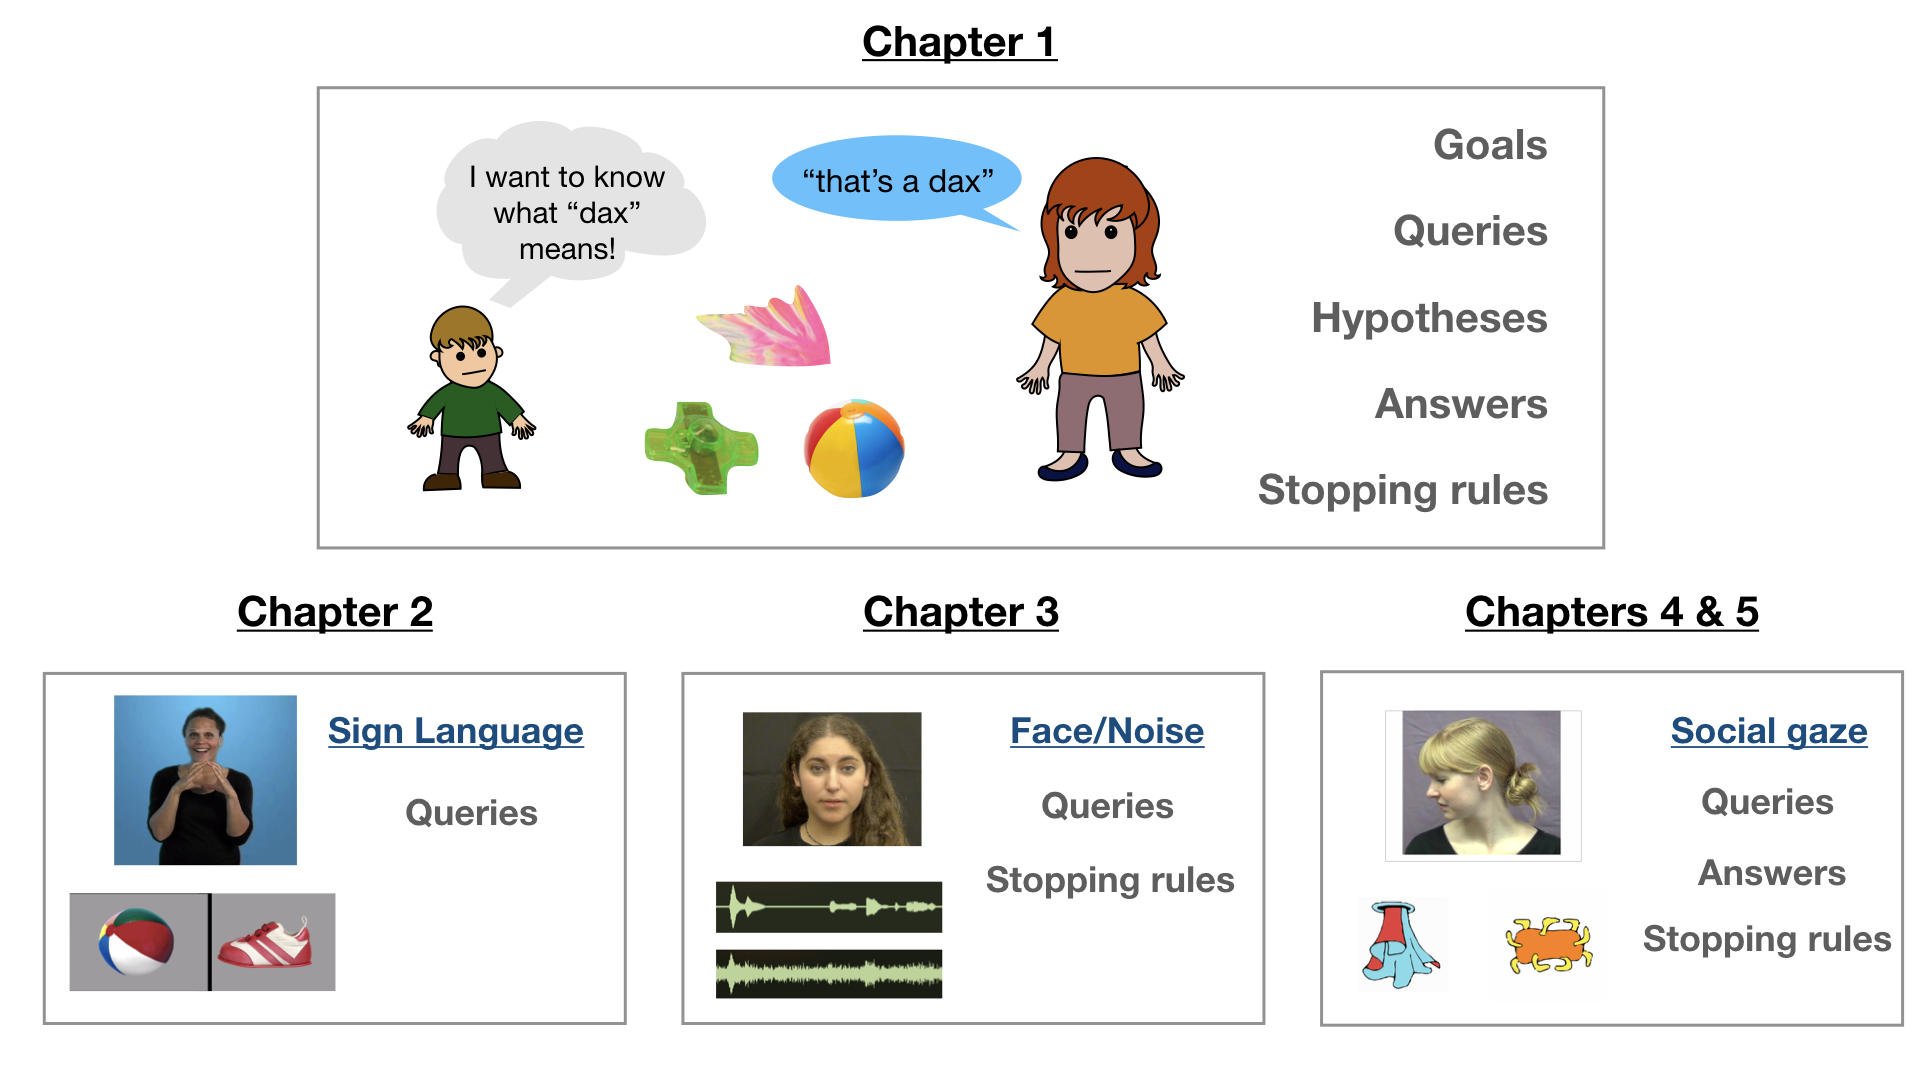
\includegraphics[width=0.9\linewidth]{/Users/ejyoon/Documents/Documents/Research/dissertation/index/chapter_child_rmds/Intro/figs/schematic_overview} 

}

\caption[Schematic overview of the dissertation content.]{The upper panel shows a schematic overview of an integrative framework of polite language understanding based on competing social goals. The lower panels show different studies examining adults' and children's understanding of different component goals (and possible tradeoffs between them) that correspond to each chapter of the dissertation.}\label{fig:schematic-overview}
\end{figure}
\chapter{A goal-based account of polite
language}\label{a-goal-based-account-of-polite-language}

\chaptermark{A goal-based account of polite language}

\section{Introduction}\label{introduction}

Imagine that a stranger on the street approached you and asked: ``I'm
sorry to bother you, but could you tell me the way to the city hall?''
Regardless of your answer, you probably would not feel puzzled or
offended by the way in which the stranger decided to seek information
that he needs. This is in contrast with a different situation where the
stranger said to you instead: ``Tell me the way to the city hall.'' In
such case you would immediately notice the lack of politeness in his
utterance, and your response to him may be negatively affected by the
irritating oddity of the situation. Now imagine another context where a
person was wearing a new, flashy dress, and her friend thought the dress
was hideous. It may actually be more surprising if the friend truthfully
said ``Your new dress is ugly,'' than if the friend decided to lie and
say ``Your new dress is gorgeous!'' But why? Why are people expected to
speak politely, when there are alternative utterances that can convey
information about the world or the speaker's intention more directly
(``Tell me the way'') or truthfully (``Your dress is ugly'')?

Language is a virtuous tool that serves many functions. Through
language, people communicate information about the world, but also form
their social relationships and establish their identity within their
society. On one hand, some theories of language functions describe
language as a transmission device for transferring from a sender to a
receiver information that reflects context or the state of affairs
(Bühler, 1934; Jakobson, 1960; Shannon, 1948). The importance of
informativity is further emphasized in more recent, influential theories
on pragmatics of natural language, which explain how meanings beyond
literal meanings of utterances arise (Grice, 1975; Searle, 1975). On the
other hand, some linguistic theories, especially those with references
to language development, identify social roles of language that people
use to make contact with others and form relationships (Ervin-Tripp,
1967; Halliday, 1975). These theories underscore how linguistic rules
that language users tend to follow represent the norms and structure of
the community using the language (Ervin-Tripp, 1969).

Could polite speech reflect both the informational and the social roles
of linguistic communication? Previous theoretical accounts of polite
speech vary in their focus on informational versus social aspects of
polite language. Some theories view polite speech as reflecting social
rules and norms (Richard J. Watts, Ide, \& Ehlich, 1992), some as
abiding by communicative maxims that people are expected to follow in
conversations, to be both as informative and as affirmative of their
conversational partner as possible (Lakoff, 1973; Leech, 1983), and yet
some others as performing face management, or trying to maintain
interactants' good public self-image or reputation (P. Brown \&
Levinson, 1987).

In this Chapter, I propose that that polite speech highlights both
informational and social uses of language: Polite speech reflects a
principled tradeoff between the informational, epistemic content a
speaker wants to convey (e.g. ``I want you to tell me the way to the
city hall'') and other social concerns, such as prosocial or
self-presentational goal that the speaker wants to express for herself
and others (``I'm not rudely commanding you to tell me the answer, but
making a request in a respectful way''). Thus, my goal is to unify
previous theoretical frameworks in one, goal-driven account of polite
speech. In what follows, I will describe the goal-based account of
polite speech in detail (Part I), and summarize previous models and
theories of polite speech and situate them within the framework of the
current goal-driven account (Part II). Then I will examine empirical
evidence for goal-driven approach to polite speech: In Part III, I will
focus on empirical work on adult production and comprehension of polite
speech which show that adults reason about speaker goals in polite
speech; and in Part IV, I will probe empirical evidence from
developmental work that children's production and understanding of
polite speech advance as they grow older. In doing this I will show that
children's production and comprehension of polite speech is related to
the relative complexity of polite speech based on its goal tradeoff.

\section{Part I: A Goal-based account of
politeness}\label{part-i-a-goal-based-account-of-politeness}

What does it mean to speak politely? Common instances of polite speech
that occur to one's mind probably include the simplest politeness
markers, such as ``please,'' ``thanks,'' and ``sorry.'' More complicated
examples would involve ways in which, for example, a person make a
request: under normally conceivable circumstances, it would certainly be
more polite to ask ``Would it be too much trouble to ask you to complete
this survey when you're not too busy?'' than to say ``Do this survey
now.'' The word ``polite'' can sometimes carry a negative undertone in
its meaning, as in ``she was just being polite,'' which is likely to
mean the speaker was hiding her genuine beliefs or intentions to make
the listener feel good. From these examples, we can identify a few
characteristics that a polite utterance may exhibit: observance of
social rules, relatively high degree of elaborateness or indirectness,
and dishonesty or disingenuousness in the interest of others' feelings
or reputations.

More formal definitions of the term politeness also reveal common
features that polite speech shows. Cambridge and Oxford Dictionaries
respectively define what it means to be polite: ``behaving in a way that
is socially correct and shows respect for other people's feelings''; and
``courteous, behaving in a manner that is respectful or considerate of
others; well-mannered'' (``Polite,'' 2017a, 2017b). Similar to the
previous examples of polite speech, these definitions suggest politeness
involves (1) observance of social expectations and (2) respect for
others. Boyer (1702)'s The English Theophrastus: of the Manners of the
Age, compilation of texts describing the English life in the early
eighteenth century, identifies a purpose in trying to be polite:
``Politeness may be defined as a dextrous management of our Words and
Actions whereby \emph{men make other people have a better Opinion of us
and themselves} {[}emphasis added{]}.'' Thus, according to the
Theophrastus definition, speakers speak politely in order to boost the
self-images of the interactants (both the speakers themselves and their
addressees).

These common themes of politeness have been identified by previous
theoretical accounts of polite speech (reviewed in detail in Part II).
But each of the accounts only focused on certain aspects of polite
speech but disregarded others, and their explanations for politeness
have been viewed as largely disparate. Here I make a unification
proposal, where these existing approaches to polite speech can be united
under a single goal-based account of polite speech.

I propose that polite speech reflects some degree of tradeoff between
three main communicative goals: informational, prosocial, and
(self-)presentational. \emph{Informational goal} has to do with the
speaker's desire to convey the most accurate information in the most
efficient manner. \emph{Prosocial goal} is about the speaker's desire to
retain the listener's acceptable self-image as a decent individual and
as a reputable member of society. \emph{Presentational goal} reflects
the speaker's desire to present the speaker herself in a good light, to
appear to be a kind and helpful individual. Below I describe each goal
in more detail.

\subsection{Informational goal}\label{informational-goal}

A speaker's informational goal, i.e.~to prioritize information transfer
in communication, may involve two closely related notions: informativity
and truthfulness. Informativity is the notion of conveying the intended
meaning in the most efficient and precise manner possible. The idea of
informativity here is similar to Grice (1975)'s notion of cooperativity:
A speaker will cooperatively choose utterances such that the listener
can understand her intended message. Thus, the current notion of
informativity that I adopt will encompass the whole Cooperative
Principle (CP) that Grice posited (``Make your contribution such as
required by the purposes of the conversation at the moment''), and
especially the Maxim of Quantity (``Make your contribution as
informative as is required''), though Maxims of Relevance (``Be
relevant'') and Manner (``Be perspicuous''; i.e.~be brief, orderly, and
unambiguous) can also be relevant to the notion of informativity as I
discuss in this Chapter.

The idea of informativity has been formalized in probabilistic
(Bayesian) models as a utility function of a speaker with particular
goals in mind. The ``rational speech act'' (RSA) theory of language
understanding (see N. D. Goodman \& Frank (2016a) for a review) assumes
that listeners expect speakers to aim to be helpful yet parsimonious,
choosing their utterances approximately optimally based on a
communicative goal (e.g., inform the listener) and interpret an
utterance by inferring what the helpful speaker meant based on the
utterance and any other relevant information about the world. The theory
defines a standard, informative utility as the amount of information a
literal listener (\(L_0\)) would still not know about world state
(\(s\)) after hearing a speaker's utterance (\(w\)):

\[U_{epistemic}(w; s) = ln(P_{L_0}(s | w))\]

where the utterance choice is approximately rational (i.e., in
proportion to the expected utility gain) and \(w\) is chosen from a set
of alternative, relevant utterances.

For example, if Bob asked Alice ``How was my cookie?'' and Alice said to
Bob ``It was good,'' with only the goal to be informative in mind, Bob
would think that Alice was being maximally informative by using the word
``good'' instead of another relevant, stronger word such as ``amazing,''
and infer that Ann meant ``good but not amazing'' because otherwise Ann
would have used the word ``amazing'' instead.

I note here that Ann's speech act could be analyzed as having observed
the Gricean Maxim of Quantity, by making her utterance maximally
informative, and Bob's inference as being based on such assumption that
Ann's utterance is as informative as is required to meet Bob's needs.
But as the comparison between the former goal-directed analysis and this
latter maxim-based analysis may reveal, the maxim-based account is
difficult to formalize (Hirschberg, 1985) whereas the goal-directed view
allows for quantitative account of factors contributing to the
linguistic phenomena at hand (N. D. Goodman \& Frank, 2016a). From here
on, I take the goal-directed view rather than the Gricean maxim-based
view of the speaker; thus, analyses of speakers and their utterances
will be based on speakers' communicative goals to convey information,
etc., rather than their observation or violation of Gricean maxims.

Informational goal can also involve truthfulness: the meaning that
accessed by the listener should match the true state of the world as
closely as possible. In other words, the speaker will want to convey
what is true (to the extent of her knowledge), not what is false. For
example, if Bob baked some cookies and they tasted terrible, and Alice
had the goal to be truthful, she would want to convey what matches the
true state of the world as closely as possible (``Your cookies tasted
terrible''). On the other hand, if Alice remarked to Bob about his
cookies ``Your cookies tasted good,'' with goal to be informative and
truthful, the true state of the world must be such that Bob's
presentation was truly good (but probably not amazing, because otherwise
Alice would have said that it was amazing), and not bad or terrible.

As for when speakers decide not to tell the truth, there is a difference
between violating versus flouting of truthfulness (which Grice also
discusses; see Grice (1975), p.~49, 53). Flouting involves contradicting
common knowledge shared between the speaker and listener about the true
state of the world, such that the listener notices that the utterance
meaning does not match the true state. For example, after Alice and Bob
together watch a movie that was obviously gory and disturbing to both of
them, if Bob says ``well, that was a really happy, fluffy movie!'' then
his utterance would be flouting truthfulness goal, and Ann would
recognize Bob's utterance as an ironic one. On the other hand, violating
truthfulness does not hold assumption of such common knowledge of the
true state of the world, and thus the listener may not notice the
mismatch between the utterance meaning and true state of the world,
although the listener can potentially access it through other means
(e.g.~realizing that the speaker had reasons to lie). Here I will mainly
focus on violation, not flouting, of truthfulness, for example when
speakers tell white lies (i.e., when the speakers do not intend that the
listeners know what the truth is).

Speakers' informational goal to be informative and truthful may
encompass communicative cooperation in both locutionary and
perlocutionary senses. A locutionary goal deals with conveying the
intended meaning of the utterance within a conversation, whereas a
perlocutionary goal involves achieving the speaker's ultimate goals
toward the listener (Attardo, 1997). What could be an informational goal
in its perlocutionary sense? In being truthful, speakers may ultimately
want to maintain their moral obligation to tell the truth to others.
This obligation is in line with Western philosophers' argument
throughout the history that it is morally wrong to lie (Augustine, 1952;
Kant, 1949), although there have been debates on whether the degree of
wrongness may depend on context (e.g., if the speaker was telling a
white lie; Sweetser, 1987). For example, if Alice said to Bob ``Your
cookies were good,'' Alice's locutionary goal would be to convey to Bob
her intended meaning that his presentation was good (but perhaps not
amazing), whereas her perlocutionary goal would be for Bob to think that
the presentation was good, which was (apparently) the truth; Alice
thereby upholds her moral obligation to tell the truth to Bob. Alice's
goal to be truthful, then, is achieved in both locutionary and
perlocutionary senses.

Besides an informational goal, a speaker may also want to address
concerns that are social in nature: having to do with interacting and
maintaining good relationships with other people. Below I describe two
related but different goals that speakers may want to accomplish for
social reasons: prosocial and presentational.

\subsection{Prosocial goal}\label{prosocial-goal}

A prosocial goal involves the speaker's desire to to follow social norms
and make others feel happy and respected. Speakers can try to accomplish
the prosocial goal in several ways, one of which is social norm
observance: abiding by social norms and expectations. There may be
simple rules such as ``say please when you make a request'' or ``say
thanks to express gratitude,'' but sometimes the norms can be more
complex. Speakers should avoid saying utterances that are \emph{too}
polite, to the extent that the utterances become marked and are no
longer considered ``optimally polite.'' For example, a request for
opening a window by saying ``Sorry, could you open that window behind
you? Thanks.'' would be a normal, socially expected way to make the
request; but a request such as ``I'm so terribly sorry to bother you
with this irritating request, but if you don't mind, would you care to
open that window behind you, only if it's not going to be too much
trouble for you?'' would be a signal to the addressee that something in
the situation is odd and marked; either that the request involves a
higher cost than is normally expected for opening a window, or the
speaker is unusually afraid of incurring a debt to the addressee, etc.
This principle of social norm observance is then parallel to Grice's
Cooperative Principle, in that the CP outlines normative expectations
for a speaker who wants to convey information as efficiently as
possible, whereas the current principle of social norm observance deals
with normative expectations for a speaker who wants to maintain social
order. Thus, if the CP is a principle of information transfer, social
norm observance is a principle of social order. Both principles call for
unmarkedness of utterances, and when the utterances are marked due to a
violation of its rules, then the listener will try to infer reasons for
such violation.

Speakers may also try to be prosocial through face management.
\emph{Face} is a notion introduced by Goffman (1967), and represents an
individual's publicly manifest self-esteem. He argued that people
perform interpersonal rituals whereby face maintenance is a fundamental
condition of the interactions. Goffman identified two kinds of faces
that people want to maintain: \emph{positive face}, or the want for
solidarity or approval from others, and \emph{negative face}, or the
want to be free from imposition. Interactants will always want to
preserve each other's face, and so potential face threats will somehow
have to be modified. P. Brown \& Levinson (1987) suggested that a
strategy for such facework is politeness, which they defined as
deviation from Gricean informativity (described in detail in Part II).

For example, a request such as ``You couldn't possibly pass the salt,
could you?'' would be an example of negative politeness strategy (i.e.~a
strategy to save negative face; P. Brown \& Levinson, 1987, p. 136) as
the speaker is being pessimistic about the compliance of her request and
not assuming that the listener has to be willing or able to do any acts
predicated of him. On the other hand, utterances that emphasize the
common ground between the speaker and listener (i.e.~that the speaker
and listener share the same goals, values, knowledge, etc.), and address
the fulfillment of the listener's want are positive politeness
strategies; for example, ``What a beautiful vase this is! Where did it
come from?'' (P. Brown \& Levinson, 1987, p. 103) saves the listener's
positive face by attending to the listener's wants and interests. When
face management is in conflict with informational goals, the meaning of
utterance would differ depending on which goal the speaker decided to
prioritize. As described earlier, if Ann said to Bob, ``Your
presentation was good,'' and she wanted to prioritize informational
goals only, then her utterance would indicate that Bob's presentation
was truly good (though perhaps not amazing). However, if Ann spoke with
a prosocial goal to save Bob's face and wanted to boost his self-image
instead, then Bob's presentation actually could be bad rather than good.

\subsection{Presentational goal}\label{presentational-goal}

Language also reflects a speaker's goal to present themselves in a good
light, thereby saving the speaker's own face. This last goal is related
to the informational and prosocial goals previously described, in that
speakers must be mindful of the listener's want to be informed or to
maintain his positive self-image, but instead of actually \emph{being}
maximally informative or prosocial, presentational goal concerns
\emph{appearing} to care about these goals. Thus, a speaker may engage
in a recursive reasoning about a listener who thinks about a speaker who
wants to be informative and/or prosocial, and then can produce
utterances to make the listener \emph{think} that the speaker is being
informative, being prosocial, or both of those things. For example,
rather than saying ``your talk was terrible,'' people are more likely to
say ``it wasn't bad'' to \emph{indirectly} suggest that the talk was not
great, while signaling their good intention to be nice and not say the
harsh truth (see Chapter II for the formal definition and more detailed
description of the presentational goal).

\section{Part II: Previous theoretical accounts of polite
speech}\label{part-ii-previous-theoretical-accounts-of-polite-speech}

In Part II, I aim to (i) describe different classes of theoretical
approaches to the understanding of polite speech; (ii) for each class,
explain how the approach can be situated within the current proposal for
the goal-based account for polite speech; and (iii) discuss what
advantages the goal-based account can offer beyond the existing
approaches. Summary of prominent theories and their implications within
goal-based framework can be found in Table 1.1.

\newpage

\blandscape
\begin{table}

\caption[Review of existing theories of polite language]{\label{tab:lit-rev-table}Summaries of previous theoretical approaches to polite speech and their implications within the current goal-based framework.}
\centering
\resizebox{\linewidth}{!}{
\begin{tabular}[t]{>{\raggedright\arraybackslash}p{3cm}>{\raggedright\arraybackslash}p{5cm}>{\raggedright\arraybackslash}p{8cm}>{\raggedright\arraybackslash}p{8cm}}
\toprule
\textbf{Politeness as:} & \textbf{Theories offered by:} & \textbf{Summary} & \textbf{Advantage of goal-based framework}\\
\midrule
Observance of communicative maxims & Lakoff (1973); Leech (1983) & Polite speech is governed by conversational rules and principles, that are complementary to Gricean Cooperative Principle (Grice, 1975) & Gradient degree of goal tradeoff can be represented, instead of binary observance of different maxims\\
Strategy for facework & Brown \& Levinson (1987) & Speakers produce polite speech to save interactants<d5> face (positive and negative) & Clearer distinction between notions of truthfulness and informativity becomes possible, which then allows more precise analysis of goal tradeoffs\\
 & Spencer-Oatey (2000) & Speakers try to preserve interactants' face and sociality rights & \\
Social rules and norms & Watts (1989); Locher \& Watts (2005); Watts et al. (1992); Watts (2003) & Speakers use speech to perform relational work (not only face-work); speakers produce im/polite (marked) utterances and politic (unmarked, normative) utterances & No distinction between polite vs. politic utterances is necessary\\
 & Fraser \& Nolen (1981); Matsumoto (1988); Ide (1989); Mao (1994) & Speakers want to fulfill societal obligations & Facework and social obligation do not have to be mutually exclusive\\
Model of game theory & Franke \& Jager (2016); Pinker et al. (2008); Van Rooy (2003); Quinley (2011) & Speakers use polite speech to get what they want while allowing for plausible deniability, or to communicate their good intentions (while incurring cost) & Self-interest is formalized as arising from recursive reasoning that is based on genuine other-oriented goals\\
\bottomrule
\end{tabular}}
\end{table}
\elandscape

\subsection{Politeness as observance of communicative
maxims}\label{politeness-as-observance-of-communicative-maxims}

One approach to polite speech is largely based on the Gricean
perspective, and claims that conversation is driven by general
communicative principles, and politeness is a maxim (or made up of
maxims) that accompanies other principles. Whereas Grice focused on
principles that speakers follow to make their speech maximally ecient
for information transfer, he also noted: ``There are \ldots{} all sorts
of other maxims \ldots{}, such as `Be polite,' that are normally
observed by participants in talk exchanges'' (Grice, 1975, p. 47).
Searle (1975) discussed conditions of performing indirect speech acts
(e.g. ``Can you pass the salt?'') for which, he claimed, ``politeness is
the chief motivation'' (p.~76). Thus, Grice and Searle both identified
politeness as a driving factor in communication, but the concept of
politeness was largely undeveloped at the time.

The communicative maxim approach for polite speech expanded with
proposals for conversational rules and principles that govern polite
speech. Lakoff (1973) suggested a set of rules (``Don't impose,'' ``Give
options,'' ``Be friendly'') that underlie utterances that are polite,
and thus deviate from directly expressed meanings. Leech (1983)
developed a similar proposal to Lako↵'s in greater detail, proposing
Politeness Principle (PP), which is complementary to the Gricean CP.
Leech argued that the PP, like the CP, can be subclassified into more
specific maxims: Maxims of Tact, Generosity, Approbation, Modesty,
Agreement, and Sympathy. The primary postulate of the PP is that
interactants prefer to express polite beliefs, which are beliefs that
are favorable to the other person (and/or unfavorable to oneself). For
example, Approbation Maxim states that a speaker observing the PP will
minimize dispraise, and maximize praise, of the other person (e.g.
``Your dress looks gorgeous!''), whereas Modesty Maxim states that a
speaker will minimize praise, and maximize dispraise, to the speaker
herself (e.g. ``This is just a small gift, but I hope you like it''
downplaying the value of the gift). Gu (1990) proposes addition of
``Balance Principle'' to the set of politeness maxims, where favors from
A to B are balanced by favors from B to A, such that the PP can function
to maintain social equilibrium.

The theories of politeness as a communicative principle focuses on cases
of tradeoff between speakers' communicative goals: On one hand, the
speaker wants to be informative, following Gricean maxims, but on the
other hand, the speaker wants to follow social rules, represented by
Lakoff's rules or Leech's PP. An utterance then reflects some level of
both of these desires. However, there arise a classification and
quantification issue: maxims of PP are informal and categorical, which
makes it difficult to represent the degree to which the utterance
observes or violates a given maxim. In this regard, the goal tradeoff
approach is preferable to the maxim approach, for it becomes possible to
represent a gradient degree of tradeoff between speakers' goals of
informativity and social rule following.

\subsection{Politeness as strategy for
facework}\label{politeness-as-strategy-for-facework}

Another approach to analysis of polite speech that has been highly
influential is the model of politeness as face management, developed by
P. Brown \& Levinson (1987). The model is primarily based on the concept
of face (Goffman, 1967) that deals with an individual's public persona
(introduced earlier in Part 1). P. Brown \& Levinson (1987) take a
strategic approach to politeness, and focuses on strategies that
speakers employ in order to avoid, redress, or mitigate threats to face
(either the addressee's or the speaker's own). Like the communicative
maxim approach, P. Brown \& Levinson (1987)'s account also start at the
assumption of the Gricean CP, and attribute the cause of a speaker's
deviations from the CP to the speaker's desire to be polite. Thus, given
a speaker's desire to save face, the more an utterance deviates from
maximal informativity, the more ``polite'' (face-saving) the utterance
will be.

Within the goal-based framework, it can be said that P. Brown \&
Levinson (1987) recast the notion of a cooperative speaker as one who
has both an informational goal to improve the listener's knowledge state
as well as a social goal to minimize any potential damage to the
hearer's (and the speaker's own) face. With the idea of these
conflicting goals, Brown and Levinson's theory is conceptually closest
to the current proposal among all theories to be discussed.
Specifically, they primarily focus on the conflict between goals of
social face management and epistemic informativity. For example, by
saying ``Can you please open the window?'' instead of ``Close the
window,'' the speaker decides to sacrifice informativity (i.e.~maximally
efficient transfer of the intention for the addressee to open the
window) in order to save the addressee's negative face (i.e.~freedom
from imposition or order from others). Another example of negative
politeness (i.e.~strategy to save negative face) is a speaker fronting
his gift-giving by saying ``This is just a small gift'' in order to
emphasize that the listener is not incurring too much debt to the
speaker and thus not being imposed a burden to return the favor. On the
other hand, positive politeness or act of saving positive face can be
exemplified by utterances that emphasize approval of the listener's
interest or performance, e.g. ``What a fantastic garden you have!'' (P.
Brown \& Levinson, 1987, p. 104).

One drawback in P. Brown \& Levinson (1987) is that key elements
required for analysis of speakers' goals or intended meanings are
ambiguous and difficult to formalize. The core assumption of Brown and
Levinson's analysis is that deviations from Gricean maxims (that
prioritize the match between the literal and intended meanings) lead to
increase in politeness. In order to estimate the degree to which
speakers try to be polite, there should be a way to measure the degree
of deviation from the Gricean maxims (i.e.~the degree of mismatch
between the utterance surface meaning, intended meaning, and true state
of the world; see Section 1 for how these factors can be formalized
e.g.~in RSA). However, Brown and Levinson do not provide a way to
formalize the literal or intended meaning or the state of the world. For
example, it is unclear how much deviation from the Gricean maxim(s)
occurred when a speaker produced an utterance such as the example
previously mentioned: ``What a fantastic garden you have!'' Since the
authors do not provide the true state of the world (i.e.~how beautiful
the garden actually was in the speaker's opinion), it is difficult to
define or quantify the speaker's effort for politeness or the cost of
face threat the message would have involved given an alternative
utterance (``It is a mediocre garden you have.'') A clearer
identification of the true state of the world, the speaker intended
meaning, and the set of relevant alternative utterances, and a way to
formalize these elements, will help with quantificational analysis of
polite utterances.

Spencer-Oatey (2000) put forward another theory based on Goffman's
notion of face; it is a more general model of rapport management, or
management of interpersonal relations, distinguished from face
management as proposed by Brown and Levinson. Spencer-Oatey challenges
Brown and Levinson's distinction between positive and negative face, and
argues that the former involves the concept of face, or the positive
social value claimed by a person, whereas the latter does not concern
face but rather what she calls ``sociality rights,'' or a person's
entitlements in interactions with others. She then further proposes that
face management and sociality rights management each has both personal
components (concerning self-esteem and individual identity) and social
components (concerning social role and entitlements within relations
with others). Spencer-Oatey then largely focuses on speakers' attempt to
balance between general epistemic goals and both face management and
social expectations. Thus, in saying ``This is just a small gift, but I
hope you like it'' the speaker may not only be concerned about the
speaker's and the listener's faces as individuals but also the
conventional social obligations associated with gift-giving that the
speaker and listener are expected to follow through. However, similar to
Brown and Levinson's analysis, Spencer-Oatey's analysis is limited in
that it does not identify or formalize the epistemic knowledge (the
speaker intended meaning and true state of the world) behind utterances,
making it difficult to quantitatively analyze the goal tradeoffs.

\subsection{Politeness as social rules and
norms}\label{politeness-as-social-rules-and-norms}

Another set of theories for polite speech relies on the notion that
politeness deals with following social norms and expectations. One line
of theory argues for the need to distinguish between marked, strategic
polite behaviors versus unmarked, normative ``politic'' behaviors.
Richard J Watts (1989) defines ``politic'' behavior as
``socio-culturally determined behavior directed towards the goal of
establishing and/or maintaining in a state of equilibrium the personal
relationships between the individuals of a social group, whether open or
closed, during the ongoing process of interaction.'' For example, ``May
I open the window behind you?'' will be a normative, politic statement
if used in a formal setting or said to a stranger, but can be considered
marked, overly polite statement when said to a close family member.

Richard J. Watts et al. (1992) posited that examples of polite speech in
Brown and Levinson's work, such as honorifics or indirect speech acts,
will be considered ``polite'' only if they go beyond their normal usage
as socio-culturally constrained forms of politic behavior. For example,
according to Watts, responding to an offer ``Would you like some more
co↵ee?'' by nonsaliently saying ``Yes, please.'' (Richard J Watts, 2003,
p. 186) should be considered a politic behavior. On the other hand, if
the response is instead ``Yes, please, that's very kind, coffee would be
wonderful.'' Culpeper (2011) is considered to be polite as it is
``perceived to go beyond what is expectable'' (Richard J Watts, 2003, p.
19). Based on these observations, Locher \& Watts (2005) claim that, a
better approach than Brown and Levinson's ``facework'' to encompass all
degrees of polite speech will be a larger ``relational work'' that
considers all-ranging levels of politeness from marked im/polite to
unmarked politic utterances.

Watts and colleagues' claim can be re-framed as calling for the need to
consider wide-ranging informational-social tradeoffs. Watts' distinction
between politic versus polite speech lies in whether the addressee
recognizes and pays attention to the divergence between speakers'
informational and social goals, as revealed by the discrepancy between
literal versus intended meaning, and tries to infer the intended
meaning. For politic utterances, the mismatch between literal and
intended meaning is unmarked and thus remains unnoticed; For polite
utterances, the mismatch is salient and the listener is called to pay
attention to the reason for that mismatch, and to infer what a speaker
was truly trying to say or what the speaker truly believed (i.e.~the
true state of the world).

One benefit of the current goal-based account over Watts et al.'s claim
is that there is no need to classify different kinds of polite speech as
different categories (polite vs.~politic). Rather, by observing how
subtle changes in the literal meaning, intended meaning, or the true
state of the world can lead to changes in a speaker's inferred goals or
evaluation of politeness, one can examine the phenomenon as a whole.
Watts et al.'s theory makes it rather dicult to know exactly what
utterances count as polite vs.~politic; for example, should the
utterance ``This is just a small gift, but I hope you like it'' produced
in a gift-giving act be considered politic or polite? The goal-based
framework obviates this need and quantifies the relative degree of
politeness in terms of goal tradeoff.

Other theorists have focused on speakers' attempt to abide by societal
obligations and expectations, explicitly distinguishing between their
accounts and ``strategic'' approach to politeness based on individual
goals (e.g., P. Brown \& Levinson, 1987). Fraser \& Nolen (1981) put
forth an account for politeness based on the idea of ``conversational
contract'' (CC), which posits that interactants bring a set of rights
and obligations to the conversation. Observance of these obligations,
according to these authors, are not strategic but rather ``getting on
with the task in hand in light of the terms and conditions of the CC''
(Fraser, 1990, p. 233). Critiques of polite speech analysis based on
facework by sociolinguists (Ide, 1989; Mao, 1994; Matsumoto, 1988)
assert the importance of considering speakers' desire to fulfill
societal obligations. They go against Brown and Levinson's notion of
``negative face'' as it is heavily loaded with the assumption of
individuality as opposed to group identity, which especially becomes
prominent in East Asian cultures and languages. Thus, they may argue
that an utterance such as ``This is just a small gift, but I hope you
like it'' in East Asian cultures may not reflect an attempt to save the
listener's negative face, but to follow convention based on their
assigned role (e.g.~within a hierarchical social structure).

The proponents of social obligation approach for politeness focus
primarily on speakers' prioritization of observance of social norms over
informarional goals. This approach rejects the assumption of
universality of face management principles claimed by Brown and
Levinson, and argues that in some cultures the need for face-work
(especially for individuality) may be weak or non-existent. Instead, a
speaker may desire to follow and reinforce social norms and
expectations, and decide how to balance between that desire and the goal
to transfer information. For example, if a professor is to accompany his
long-time mentor to a restaurant, when it comes to time to pay, the
professor may say ``I insist, you should let me pay for this - please
treat me next time'' despite thinking that he doesn't actually want to
pay the bill, because it is more important to hide his genuine
intentions to abide by what is expected of him as as a lower-status
individual.

The goal-based framework aims to simultaneously acknowledge the
importance of these theories identifying more subtle cases of politeness
and unify them with the work for face-saving strategies (e.g., P. Brown
\& Levinson, 1987) they largely argue against. Whereas the social
obligation theories attempt to reject the facework-based accounts of
polite speech, the current proposal is that speakers consider both
social obligation and facework as potentially important social goals,
and try to balance between these social goals and epistemic goals to
convey their message. Thus, instead of presuming mutual exclusivity of
speakers' goals either to save face or to abide by social rules, the
goal-based framework instead assumes that both goals can apply
simultaneously, to different degrees depending on the cultural or
conversational context.

\subsection{Politeness in the game-theoretic
approach}\label{politeness-in-the-game-theoretic-approach}

Finally, there have been recent attempts to analyze polite speech from a
game-theoretic perspective, which assumes that individuals interact with
each other in an effort to achieve their own goals. A few proponents of
game-theoretic approach have analyzed indirect speech as a whole,
viewing polite indirect utterances as a subset. Franke \& Jäger (2016)
argue that indirect speech used for demands results in greater
likelihood of compliance from the other party, as indirect speech
suggests higher stakes for the listener in case the speaker's wants are
not fulfilled. For example, a mobster who is trying to take protection
money from a restaurant owner could pose a veiled threat by saying:
``Your little daughter is very sweet. She goes to the school in Willow
Road, I believe'' (Franke \& Jäger, 2016, p. 19). This indirect speech
is used to communicate that the restaurant owner's stakes are high
because his daughter can get hurt if he does not pay the money, whereas
mobster's stakes are low because he is free to do whatever he wants in
the neighborhood. Franke \& Jäger (2016)'s account thus focuses on the
reasons to be indirect to send the informational message more
effectively in the interest of the listener's observance of the
speaker's wants, though the scope of their explanation does not
explicitly cover polite speech.

Addressing a broader set of indirect utterances, Pinker, Nowak, \& Lee
(2008) describe three possible reasons for speaking indirectly: allowing
for plausible deniability and thus preventing (legal) responsibility for
the intended meaning (``Ocer, is there some way we could take care of
the ticket here?''), avoiding emotional costs of mismatch (such as
awkwardness) in perceived relationship between speaker and listener, and
generating common reference point that is qualitatively different from
direct literal meaning even when the intended meaning is clear to the
interactants (``Would you like to come up and see my etchings?'').

Other game-theoretic accounts addressed polite indirect speech
specifically, highlighting its rationality despite its potential cost.
Van Rooy (2003) argues that polite utterances are costly ``handicaps,''
which incur a social debt and reducing the social status of the speaker,
but which are rationally used to communicate good intentions to the
addressee. Quinley (2011) observes that politeness is a form of ``trust
game,'' where making a polite request is rational when assumptions of
reputation or observation are in place over multiple iterations of
conversational turns.

Game-theoretic approach is similar to the current goal-based approach in
that the theory is very much built on the notion of tradeoff of goals,
but differs in that it is ultimately focused on the speaker's goals for
the self. In game theory, a speaker's informational goals are centered
around informativity, or effective transmission of the message, to
ultimately gain the desired compliance from the other party (Franke \&
Jäger, 2016). Similarly, a game-theoretic speaker's social goals involve
face management, but less of the intent to save the listener's face and
more to save the speaker's own face, to avoid being held responsible for
disobeying the law or disrespecting someone (plausible deniability) and
to prevent high emotional costs misunderstanding common knowledge
assumed between speaker and listener (Pinker et al., 2008). The current
proposal differentiates between speakers' interest oriented toward
others (i.e., a genuine desire to inform others or save others' face),
and interest towards the speakers themselves (e.g., a desire to
\emph{appear} to be a particular way). I formalize the self-interest
based on a recursive reasoning about the other-oriented goals: Speakers
reason about listeners who imagine speakers to be genuinely informative
or kind, and then the speakers produce utterances that can portray
themselves to be such helpful individuals.

\section{Part 3: Empirical work on polite speech in
adults}\label{part-3-empirical-work-on-polite-speech-in-adults}

In previous sections, I have recapitulated previous theoretical
perspectives to make a unifying proposal that speakers consider
tradeoffs between informational and social goals (e.g., prosocial,
self-presentational). In this section, I review empirical evidence from
adult interpretation, evaluation and production of polite speech that
show their consideration of speaker's informational and social goal
tradeoff.

\subsection{Interpretation of polite
speech}\label{interpretation-of-polite-speech}

Empirical findings show that adults' interpretation of polite utterance
meanings is based on the epistemic-social goal tradeo↵ considered by the
speaker. For example, people's interpretation of seemingly irrelevant,
ambiguous utterances reveal that listeners pay attention to the
epistemic-social tradeoff, attributing politeness as a strong reason for
apparent irrelevance. T. Holtgraves (1998) examined interpretations of
replies to someone asking for an opinion on some performance that he
just gave (e.g. ``What did you think of my presentation?''), where the
replies seemingly did not directly address the questions and involved
relevance violations (``It's hard to give a good presentation''). The
author found that people often assign face-threatening meaning to the
indirect reply. Additionally, people spent longer coming up with an
interpretation when the true state was positive (the addressee actually
gave a good presentation) or when the literal meaning of the reply was
in the positive direction (``It's easy to give a good presentation''),
which thus made face management an unlikely goal. These findings overall
indicate that people identify face management as a key motivation for
violating the informativity goal, and struggled when face management was
no longer a valid reason for violation of the goal to be informative to
the listener.

Another prominent example of polite speech interpretation in line with
the idea of the speaker's goal tradeoff consideration comes from
empirical work on cancellation of pragmatic inferences that are normally
in force in non-face-threatening, low-stakes contexts. People's
inferences change for non-literal meanings of various quantifiers
depending on the presence or severity of face threat toward the
listener. For example, the term ``possibly'' could be used to convey a
probability greater than 0 and up to 1 in its literal sense, but usually
people assume that it denotes a probability that is neither too high nor
too low. This is because people assume that a speaker would use
quantifiers in the most efficient, informative way possible (Grice,
1975), and if the speaker wanted to convey a greater certainty then she
would have used a stronger term, such as ``certainly.''

However, when the situation involves a potential face threat or a high
stake for the listener, the speaker would have a reason to be more
vague, to accommodate for face-saving or plausible deniability. Indeed,
Bonnefon and colleagues found that people interpret the word
``possibly'' as implying a greater likelihood when it is used to
describe a condition of a higher stake (e.g. ``You will possibly suffer
from deafness soon'' or ``Your pain is possibly going to increase'')
than a lower stake (``You will possibly suffer from insomnia soon'' or
``Your pain is possibly going to decrease''; Bonnefon \& Villejoubert
(2006); Pighin \& Bonnefon (2011)).

Similarly, people's interpretation of other quantifier phrases such as
``some'' and ``A or B'' differ depending on the contexts. People usually
endow upper-bounded meanings to ``some'' and ``A or B'' in
non-face-threatening contexts assuming speakers' epistemic
cooperativeness (Breheny, Katsos, \& Williams, 2006; e.g., Huang \&
Snedeker, 2009): ``I ate some of the cookies'' is interpreted to mean
``\ldots{} some of the cookies but not all,'' and ``she ate the cake or
the salad'' to mean ``\ldots{} the cake or the salad but not both.'' In
situations involving face threat, however, people make different
inferences: ``some'' and ``or'' in ``some of the audiences hated your
talk'' and ``We will cut your salary or take away your company car'' are
interpreted in their broader sense (``some and possibly all'' and ``A or
B and possibly both''; Bonnefon et al., 2009; Feeney \& Bonnefon, 2013).
Furthermore, a long pause before the utterance, signaling expectation of
bad news to the listener, heightened the effect for the polite
interpretation of ``some'' (Bonnefon, Dahl, \& Holtgraves, 2015). In
sum, people infer different non-literal intended meanings depending on
the context, since the speaker is expected to focus more towards social,
face-saving goal than towards epistemic goal in the presence of
potential face threats.

\subsection{Evaluation of polite speakers'
intentions}\label{evaluation-of-polite-speakers-intentions}

People's evaluation of strategies to be polite is also based on the
balance of epistemic-social tradeoffs. H. H. Clark \& Schunk (1980)
showed that people rate politeness of requests differently depending on
how much the literal meaning of indirect requests would benefit the
listener or reduce the cost to the listener. For example, requests that
implied that the speaker asked for the listener's permission (``May I
ask you?'') were rated as relatively more polite, whereas those requests
that assumed the listener's obligation to reply to the speaker (and
therefore incurs a cost for the listener; ``Shouldn't you tell me?'')
were rated as more impolite. Thus, with the increase of the maintenance
of the listener's face, to be free of imposition or obligation in this
case, relative to the degree of message transfer (i.e.~access to the
intended meaning that was assumed to be constant; e.g. ``Tell me the way
to Jordan Hall''), people's judgment for politeness of requests also
increased.

Interestingly, hints that seem to prioritize face-saving due to its
relatively high degree of indirectness are not always evaluated as most
polite. According to P. Brown \& Levinson (1987)'s rank ordering of
polite strategies, hints (i.e.~indirect speech with meanings that are
``off the record'') are supposedly more polite compared to other
politeness strategies. However, empirical evidence is divided on this
issue (e.g., Pinker et al., 2008; Terkourafi, 2002; K. Yu, 2011). For
example, Blum-Kulka (1987) found that people rate conventional indirect
requests (e.g. ``Would you mind moving your car?'') as more polite than
direct orders (``Move your car'') or hints (``We don't want any
crowding''). Along similar veins, among possible replies to a question
asking for an opinion on a newly bought dress, people perceive evasive
replies (e.g. ``It seems like clothes are getting terribly expensive'')
to be better than direct utterances (``I don't think it looks very good
on you'') or hints that sound irrelevant (``I'm going to take my
vacation next month''; T. Holtgraves, 1986).

One potential reason why hints and irrelevant remarks are not evaluated
as best politeness strategies is that they focus too much on face-saving
but not information transfer, leading to a poor balance in
epistemic-social tradeoff. Indeed, based on the results of her study,
Blum-Kulka concluded that politeness is ``interactional balance achieved
between two needs: The need for pragmatic clarity and the need to avoid
coerciveness.'' This is in agreement with the current argument that
people consider both the epistemic and social goals as important in
communication, and the balance between these two goals determines what
is optimally ``polite''.

\subsection{Production of polite
speech}\label{production-of-polite-speech}

Adult production of polite utterances reveal their attempt to balance
between epistemic and social goals. Adults spontaneously produce
requests in polite forms that do not convey their message in the most
direct manner (H. H. Clark \& Schunk, 1980). Even in situations of
conflict, people try to balance between their desire to convey their
message and desire to control their politeness level; indeed, speakers
exhibit politeness strategies even while arguing, preventing unnecessary
offense to their interactants (T. Holtgraves, 1997).

Sometimes people decide to compromise the level of unambiguity or
certainty that is communicated to the listener due to social reasons. T.
Holtgraves \& Perdew (2016) tested what degree of (un)certainty with
which people would communicate potentially face-threatening information.
They found that if the event referred to was more severe (and therefore
there is greater face threat involved) or if the person whose face was
under threat was the listener (as opposed a third party) participants
used terms with greater uncertainty. Thus, when there is a greater risk
for face threat, and therefore more reason to prioritize face
management, speakers sacrifice information transfer and convey
information more ambiguously.

Situational factors can also lead speakers to prioritize epistemic
versus social goals differently. P. Brown \& Levinson (1987) claimed
that the degree of the face-threat of an act is determined by three
factors: the listener's power status with respect to the speaker; the
degree of social distance between the speaker and the listener; and the
degree of imposition of the act (which may be culturally determined).
Thus, a speaker's attempt to minimize face threat would increase as
these three factors increase in magnitude. If their claim is true,
within the goal-based framework, speakers would prioritize face-saving
goal relatively more as the effect of these sociological factors
increase.

Indeed, empirical evidence suggest that the lower power status of a
speaker, and requests with greater imposition, lead to greater degree of
face-saving (Blum-Kulka, Danet, \& Gherson, 1985; T. Holtgraves \& Yang,
1992; Leichty \& Applegate, 1991; Lim \& Bowers, 1991). For example, in
Lim \& Bowers (1991)'s study, participants were asked to write down
their probable utterances in an imaginary situation involving a
potential face threat and varying degrees of power status of the
listener. The results showed that participants produced more ``tactful''
utterances with more indirect expression of amount of imposition on the
listener (e.g. ``I'd greatly appreciate it if you could write the paper
on behalf of the whole group'') in a scenario involving equal power
between the speaker and listener than when the speaker had higher power
than the listener (e.g. ``I know it's imposing a lot, but you gotta
write the paper again'').

Empirical work on the effect of distance on politeness has been more
inconsistent where some report results that are consistent with Brown
and Levinson's claim that greater distance leads to higher levels of
politeness (T. Holtgraves \& Yang, 1992), while others report the
opposite (Baxter, 1984; R. Brown \& Gilman, 1989). One potential reason
for the inconsistency can be that social distance may be confounded with
affect (i.e.~how much the speaker likes the listener). Nonetheless,
regardless of the directionality, all three variables of power,
distance, and degree of imposition affect speakers' politeness level; in
other words, speakers consider these factors to determine how much
priority they should place on social goal to save the listener's face as
opposed to epistemic goal to effectively convey their message.

In sum, empirical work with adults reveal that people interpret,
evaluate, and produce polite speech in ways that are consistent with the
notion of the epistemic-social goal tradeoff.

\section{Part 4: Empirical work on polite speech in
children}\label{part-4-empirical-work-on-polite-speech-in-children}

In this section, I argue that children's acquisition of polite speech
shows a pattern consistent with the goal-based account: Children show
early competence with polite speech that involves minimal conflict
between speaker goals, and gradually learn to produce and understand
polite speech with more complex patterns of competition between speaker
goals.

\subsection{Rule-based polite speech}\label{rule-based-polite-speech}

Theories on children's sensitivity to conventional rules predict
children's early understanding of simple, rule-based politeness
(i.e.~that does not involve explicit conflict between a speaker's
epistemic and social goals). In the domain of morality, Turiel (1977)
argued that children's early-emerging understanding of social
conventions is primarily based on rules and actions enforced by social
authorities, and then the development of a more flexible
person-orientation occurs throughout childhood. In other words, children
may first start by following simple moral rules such as ``do not cheat''
or ``do not steal,'' but as they grow older they may become more
flexible as they consider more complex circumstances depending on the
needs of the individuals and society involved. In the context of polite
speech, children may show similar developmental trajectory: they could
first faithfully follow rules such as ``say please'' or ``do not lie,''
but as they become more sensitive to intricate demands of different
individuals and contexts, they may start to try to balance between
different goals to satisfy those demands. According to this hypothesis,
children should start to show mastery of rule-based polite utterances,
such as syntactic politeness markers (e.g. ``please'') and conventional
request forms (e.g. ``Can you \ldots{}''), earlier than other more
complex forms of polite speech (e.g.~white lies).

Indeed, children start producing rule-based polite utterances early.
From very early on, parents teach children to be polite by following
normative rituals to say ``please'', ``thank you'', ``hello'' and
``good-bye'' (Gleason, Perlmann, \& Greif, 1984). Children start
producing the simple polite marker ``please'' early at 2.5 years (Read
\& Cherry, 1978) and request forms increase in their variety and
frequency with age (E. Bates, 1976; E. Bates \& Silvern, 1977; Bock \&
Hornsby, 1981; Ervin-Tripp, 1982; Nippold, Leonard, \& Anastopoulos,
1982).

Young children learn to produce these utterances with appropriate levels
of politeness depending on context (Ryckebusch \& Marcos, 2004; e.g.,
Snow, Perlmann, Gleason, \& Hooshyar, 1990). For example, children use
different forms of requests depending on how they are instructed to make
the requests. At three years, children start using different forms of
request when they are instructed to ``tell'' versus ``ask'' an addressee
to give them a puzzle piece (Bock \& Hornsby, 1981). Similarly,
five-year-olds are able to modify requests depending on whether they are
asked to make a request in a nice versus bossy way (Becker, 1986). E.
Bates \& Silvern (1977) showed that even two-year-olds were able to
modify their requests to make them more polite, when they were
instructed to make a request to an old lady and then ask her again ``in
the nicest way possible.'' However, children as old as seven fail to
differentiate the meaning of ``ask'' and ``tell'' when asked Ervin-Tripp
(1977) which suggests that production of context-relevant polite speech
seems to precede the precise, conscious understanding of goals for
speaking politely or impolitely.

Children are also able to adjust the level of politeness based on the
listener age and status. Even at two years, children use a polite form
of request (e.g. ``Can I have\ldots{}'') to an adult but an imperative
form (e.g. ``Give me\ldots{}'') to a peer (Corsaro, 1979; Shatz \&
Gelman, 1973). Children around 2.5 years were to found to use less
polite language with their fathers compared to their mothers
(Ervin-Tripp, Guo, \& Lampert, 1990; Ervin-Tripp, O'Connor, \&
Rosenberg, 1984). These production behaviors are consistent with Brown
and Levinson's prediction that a speaker's need for politeness strategy
will be heightened as the addressee's power status increases.

Furthermore, children make polite requests based on the degree of
imposition of their demands, and respond sensitively to the resistance
to get what they want. By five years, children produce polite speech
that matches the cost of the request they make, using more polite forms
of requests for apparently more costly impositions (Ervin-Tripp et al.,
1990). James (1978) showed that four-year-olds adjusted commands to make
them more polite toward older addressees, whereas when they had to make
requests for getting what they want (which places higher cost on the
speaker if the request is not met) children made the utterances
maximally polite regardless of the listener status. Axia \& Baroni
(1985) showed that seven-year-old Italian children were able to adjust
the polite level of request depending on resistance. Additionally,
children in preschool years and older have been observed to repeatedly
use the word ``please'' in their pleading to resistant mothers and
peers, as strategies to get what they want (Finley \& Humphreys, 1974;
Kyratzis \& Guo, 2001; Wilson \& Wood, 2004). Thus, children use
politeness as a strategy to gain compliance for their goal in the
intended message.

Comprehension of rule-based polite speech also seems to emerge early,
though evidence is more gradual and controversial compared to
production. Initial evidence seemed to suggest that producing a request
with ``please'' is judged to be polite by three years of age (E. Bates,
1976; E. Bates \& Silvern, 1977). However, in a study by Nippold et al.
(1982), this judgment of ``please'' as polite was only replicated
starting at five years of age, but not younger. Furthermore, in the same
study, children did not differentiate between requests that adults
judged to differ in politeness level (e.g. ``Give me some candy,
please'' vs. ``Can you give me some candy, please?'') until seven years
of age. But these initial studies have a few unresolved issues,
including the lack of statistical tests to assess each age group's
performance and lack of systematic manipulation of cues other than
syntax (e.g., voicing or facial expressions). Thus, more evidence is
required to confirm early understanding of conventional polite requests,
but preliminary evidence so far suggests that children start to show
some understanding of these requests before preschool years.

\subsection{Indirect speech}\label{indirect-speech}

Now I turn to children's production and understanding of polite speech
that is more complex than simple rule-based utterances and reflects a
strategic tradeoff between speaker goals. First, what do we know about
children's understanding of indirect speech, where informativity is
compromised for social goals?

Despite the wealth of studies looking at conventional indirect requests
and simple polite markers (``please''), very few studies have looked at
children's understanding of non-conventional indirect requests
(e.g.~hints); there is only limited evidence that comprehension of
under-informative indirect requests is more dicult and is acquired at a
later age than conventional requests. Bernicot and colleagues have
tested French-speaking children's abilities to evaluate implications of
requests for which the intended meaning is distinct from the literal
meaning. Bernicot \& Legros (1987) tested children's ability to
understand implications of directives in different forms: direct
directives (e.g. ``Give me the spade'') versus nonconventional indirect
directives (``I can't make a castle with my hands''). They found that
even by six years, children have diculty judging what would be an
appropriate reaction by the speaker when the addressee does not comply
with the directives. Bernicot, Laval, \& Chaminaud (2007) found some
evidence that by eight years, children are able to infer appropriate
responses to nonconventional requests in the form of hints. Finally,
ten-year-old children, similar to adults (as shown in Blum-Kulka, 1987),
judge that conventional indirect requests are the ``right thing to say''
more often compared to direct orders or hints, whereas five- and
seven-year-olds do not show this metapragmatic reasoning (Bernicot,
1991).

\subsection{White lies}\label{white-lies}

Next I consider another category of polite utterances reflecting
speakers' goal tradeoff: white lies. Children start producing white lies
early on. Talwar and colleagues have shown the earliest evidence of
white lie-telling in children: They found that the majority of three- to
seven-year-old child participants in their studies told white lies and
stated that an adult ``looks okay for the picture'' even though she has
a conspicuous mark of lipstick on her nose (Talwar \& Lee, 2002), or
lied to a gift-giver about her gift that they actually found undesirable
(Talwar, Murphy, \& Lee, 2007).

Though they produce white lies early, young children's understanding of
goals for production of white lies seems limited. When the participants
in Talwar and colleagues' studies were asked for reasons why they
decided to tell white lies, many stated they did not know why.
Similarly, Italian children of same age group struggled to predict what
the protagonist of a story might say in a situation where telling truth
would not be polite (Airenti \& Angeleri, 2011). Although there was an
increase in the proportion of correct responses with age, even
six-year-olds did not predict the correct response above chance unless
they were given an additional cue to think about politeness-related
reasons. Thus, despite the evidence of early spontaneous production of
white lies in familiar situations, children seem to have limited
understanding of goals behind white lie-telling.

Studies of comprehension and evaluation of white lies show that young
children are more charitable toward prosocial lies compared to other
kinds of lies. Evidence suggests that by four years, children perceive
prosocial lies as better than malicious lies (Bussey, 1999), and they
rate lies as nicer than truths in politeness situations (M. Song \&
Song, 2014). G. D. Heyman, Sweet, \& Lee (2009) observed that 7- to
11-year-old children rated lie-telling more favorably in politeness
situations (e.g.~a teacher gave the protagonist an undesirable gift)
than in transgression situations (e.g.~the protagonist damaged a library
book). This tendency to rate prosocial lies positively increases with
age (Walper \& Valtin, 1992).

Children's favorable perception of white lies tends to depend on their
recognition of speaker goals and reasons for white lie-telling. When G.
D. Heyman et al. (2009) asked participants for explanations of their
evaluation of the protagonist's behavior (telling a lie or truth) in
politeness context, the participants were more likely to rate
lie-telling more favorably and truth-telling more negatively when their
focus was on the impact of the statement on others rather than the
veracity of statements. Studies in other countries have also found that
children in elementary school years view lie-tellers more positively if
the lie is told in a public, face-threatening situation (Ma, Xu, Heyman,
\& Lee, 2011), or is intended to benefit others rather than the speaker
herself (Fu, Heyman, Chen, Liu, \& Lee, 2015). Overall these findings
show children evaluate white lies and blunt truths differently based on
which communicative goal or intention is prominent in the given context.

As they get older, children make more subtle inferential judgments about
implications of white lies, which shows their ability to identify
epistemic and social goals as separate intentions manifested in white
lies. Children become able to differentiate between various traits of a
speaker based on her goal tradeoff decision. Xu et al. (2013) told 7- 9-
and 11-year-old Chinese children stories of lie-tellers and
truth-tellers with either intent of helping or harming the addressee,
and looked at their ratings of benevolence and trustworthiness of the
speaker. The participants rated helpful characters (both lie-tellers and
truth-tellers) as nice and harmful characters as mean; for trust
evaluations, younger children relied more on honesty whereas older
children relied more on the intentions. This finding reveals an
interesting trend in which children of younger ages are more narrowly
focused on the speaker's truth-telling goal, whereas older children
consider the goal tradeoff more holistically and gradually shift their
preference toward the face-saving goal. Indeed, in another study by Xu,
Bao, Fu, Talwar, \& Lee (2010), Chinese children from the same age group
who considered both honesty and politeness issues in evaluating white
lie-tellers tended to tell a white lie more often than those who focused
on only one of the two issues.

\subsection{Summary}\label{summary}

In sum, the development of production and understanding of polite speech
show predicted trajectories based on the currently proposed goal-based
account. A greater degree of conflict or tradeoff between the speaker's
informational and social goals leads to more challenging cases of polite
speech that are more difficult to produce or comprehend. Thus, from
early on, children produce and understand many instances of rule-based
polite speech using simple markers of politeness, involving minimal
conflict between epistemic and social goals. As for indirect speech and
white lies, cases that reflect speakers' decisions based on the goal
tradeoff, younger children before elementary school years show only
limited understanding of motivation behind these more complex
utterances. Finally, school-year children become competent at
identifying reasons for both truth-telling (for epistemic reasons) and
prosocial lie-telling (for social reasons) and making informed
evaluations of speakers based on their tradeoff decisions.

\section{Conclusions}\label{conclusions}

In this Chapter I argued for a goal-based account of polite speech, in
which speakers consider their competing social goals (informational,
pro-social, and self-presentational goals) to speak politely. The
goal-based approach provides a way to unify previous theoretical
frameworks for polite speech, and is consistent with empirical evidence
in adults' and children's production and comprehension of polite speech.

In Chapters 2 through 4, I will present empirical evidence from adults
and children to support the goal-based account of polite speech. Chapter
2 presents a formal model of how polite speech emerges. We explored how
speakers are expected to speak politely in situations where they are
asked to provide feedback for the addressee's performance (e.g., poem
recital). We built a computational model based on the assumption that
speakers should consider goals to be informational, pro-social and
self-presentational in speaking politely (as addressed in Chapter 1),
and we show that our model successfully captures important patterns of
adult predictions for polite speech (e.g., white lies and indirect
speech).

Chapters 3 and 4 examine children's understanding of polite speech. In
Chapter 3, we look at whether 2- to 4-year-old children are able to
understand that speakers account for prosocial goals in their speech, by
examining their evaluation of polite requests (e.g., ``Can you please
pour me more water?''). In Chapter 4, we investigate whether children
reason about tradeoff between different goals (e.g., informativity
vs.~prosociality) by looking at their evaluation of white lies (e.g.,
``Your cookie was tasty'') versus blunt truths (``Your cookie was
yucky'').

The primary goal of this dissertation, then, is to probe whether and how
adults and children reason about polite speech as reflecting competing
social goals, such as goals to be informative, to be kind to others, and
to present oneself in a good light, and tradeoffs between these goals.

\chapter[Adults consider tradeoffs between competing social goals to
predict polite language use]{\texorpdfstring{Adults consider tradeoffs
between competing social goals to predict polite language use\footnote{This
  chapter is submitted and currently under review at \emph{Open Mind},
  and is joint work with Michael Henry Tessler, Noah D. Goodman and
  Michael C. Frank.}}{Adults consider tradeoffs between competing social goals to predict polite language use}}\label{adults-consider-tradeoffs-between-competing-social-goals-to-predict-polite-language-use}

\chaptermark{Modeling polite speech}

Language is a remarkably efficient tool for transmitting information.
Yet human speakers make statements that are inefficient, imprecise, or
even contrary to their own beliefs, all in the service of being polite.
What rational machinery underlies polite language use? In this Chapter,
I present evidence that polite speech emerges from the competition of
three communicative goals: to convey information, to be kind, and to
present oneself in a good light. We formalized this goal tradeoff using
a probabilistic model of utterance production, which predicts human
utterance choices in socially-sensitive situations with high
quantitative accuracy, and I show that our full model is superior to its
variants with subsets of the three goals.

\section{Introduction}\label{introduction-1}

We rarely say exactly what's on our mind. Although ``close the window!''
could be an effective message, we dawdle by adding ``can you
please\ldots{}?'' or ``would you mind\ldots{}?'' Rather than tell an
uncomfortable truth, socially-aware speakers lie (``Your dress looks
great!'') and prevaricate (``Your poem was so appropriate to the
occasion''). Such language use is puzzling for classical views of
language as information transfer (Bühler, 1934; Frank \& Goodman, 2012;
Jakobson, 1960; Shannon, 1948). On the classical view, transfer ought to
be efficient and accurate: Speakers are expected to choose succinct
utterances to convey their beliefs (Grice, 1975; Searle, 1975), and the
information conveyed is ideally truthful to the extent of a speaker's
knowledge. Polite speech violates these basic expectations about the
nature of communication: It is typically inefficient and
underinformative, and sometimes even outright false. Yet even young
speakers spontaneously produce requests in polite forms (Axia \& Baroni,
1985), and adults use politeness strategies while arguing (T.
Holtgraves, 1997), even though polite utterances may risk high-stakes
misunderstandings (Bonnefon, Feeney, \& De Neys, 2011).

If politeness only gets in the way of effective information transfer,
why be polite? Clearly, there are social concerns, and most linguistic
theories assume utterance choices are motivated by these concerns,
couched as either polite maxims (Leech, 1983), social norms (Ide, 1989),
or aspects of a speaker and/or listener's identity, known as \emph{face}
(P. Brown \& Levinson, 1987; Goffman, 1967). Face-based theories predict
that when a speaker's intended meaning contains a threat to the
listener's face or self-image (and potentially the speaker's face), her
messages will be less direct, less efficient, and possibly untruthful.
Indeed, listeners readily assume speakers' intentions to be polite when
interpreting utterances in face-threatening situations (Bonnefon et al.,
2009). How this socially-aware calculation unfolds, however, is not well
understood. When should a speaker decide to say something false (``Your
poem was great!'' based on an example from Bonnefon et al. (2009))
rather than just be indirect
(\emph{Some of the metaphors were tricky to understand.})? How does a
speaker's own self-image enter into the calculation?

We propose a utility-theoretic solution to the problem of polite
language use by quantifying the tradeoff between competing communicative
goals. In our model, speakers attempt to maximize utilities that
represent their communicative goals: informational utility---derived via
classical, effective information transmission; social utility---derived
by being kind and saving the listener's face; and self-presentational
utility---the most novel component of our model, derived by appearing in
a particular way to save the speaker's own face. Speakers then produce
an utterance on the basis of its expected utility (including their cost
to speak). The lie that a poem was great provides social utility by
making the writer feel good, but does not provide information about the
true state of the world. Further, if the writer suspects that the poem
was in fact terrible, the speaker runs the risk of being seen as
uncooperative.

We assume that speakers' utilities are weighed within a probabilistic
model of pragmatic reasoning: the Rational Speech Act (RSA) framework
(Frank \& Goodman, 2012; N. D. Goodman \& Frank, 2016a). Speakers are
modeled as agents who choose utterances by reasoning about their
potential effects on a listener, while listeners infer the meaning of an
utterance by reasoning about speakers and what goals could have led them
to produce their utterances. This class of models has been effective in
understanding a wide variety of complex linguistic behaviors, including
vagueness (Lassiter \& Goodman, 2017), hyperbole (Kao, Wu, Bergen, \&
Goodman, 2014), and irony (Kao \& Goodman, 2015), among others. In this
framework, language use builds on the idea that human social cognition
can be approximated via reasoning about others as rational agents who
act to maximize their subjective utility (Baker, Saxe, \& Tenenbaum,
2009), a hypothesis which has found support in a wide variety of work
with both adults and children (e.g., Jara-Ettinger, Gweon, Schulz, \&
Tenenbaum, 2016; S. Liu, Ullman, Tenenbaum, \& Spelke, 2017).
\begin{figure}[!t]

{\centering 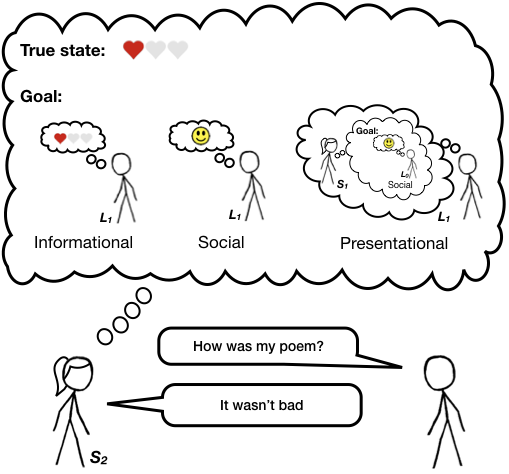
\includegraphics[width=0.9\linewidth]{/Users/ejyoon/Documents/Documents/Research/dissertation/index/chapter_child_rmds/ch2_modeling_polite/files/model} 

}

\caption{Diagram of the model: The polite speaker observes the true state and determines her goal between three utilities (informational, social, and presentational), and produces an utterance.}\label{fig:model}
\end{figure}
RSA models are defined recursively such that speakers \(S\) reason about
listeners \(L\), and vice versa. We use a standard convention in
indexing and say a pragmatic listener \(L_1\) reasons about what
intended meaning and goals would have led a speaker \(S_1\) to produce a
particular utterance. Then \(S_1\) reasons about a \emph{literal
listener} \(L_0\), who is modeled as attending only to the literal
meanings of words (rather than their pragmatic implications), and hence
grounds the recursion. The target of our current work is a model of a
polite speaker \(S_2\) who reasons about what to say to \(L_1\) by
considering informational, social, and self-presentational goals
(Figure~\ref{fig:model}).

We evaluate our model's ability to predict human utterance choices in
situations where polite language use is expected. Imagine Bob recited a
poem and asked Ann how good it was. Ann (\(S_2\)) produces an utterance
\(w\) based on the true state of the world \(s\) (i.e., the rating, in
her mind, truly deserved by Bob's poem) and a set of goal weights
\(\hat{\phi}\), that determines how much Ann prioritizes each of the
three possible goals. Ann's production decision is softmax, which
interpolates between maximizing and probability matching (via
\(\lambda_{S_2}\); N. D. Goodman \& Stuhlmüller, 2013):

\[P_{S_2}(w | s, \hat{\phi}) \propto \exp(\lambda_{S_2} \cdot \mathop{\mathbb{E}}[U_{total}(w; s; \hat{\phi}; \phi_{S_1})]).\]

We posit that a speaker's utility contains three distinct components:
informational, social, and presentational. The total utility
\(U_{total}\) of an utterance is thus the weighted combination of the
three utilities minus the utterance cost \(C(w)\):

\[U_{total}(w; s; \hat{\phi}; \phi_{S_1}) = \phi_{inf} \cdot U_{inf}(w; s) + \phi_{soc} \cdot U_{soc}(w) + \phi_{pres} \cdot U_{pres}(w; \phi_{S_1}) - C(w).\]

We define \emph{social utility} (\(U_{soc}\)) as the expected subjective
utility of the state \(V(s)\) implied to the pragmatic listener by the
utterance: \(U_{soc}(w) = \mathbb{E}_{P_{L_1}(s \mid w)}[V(s)]\). The
subjective utility function \(V(s)\) could vary by culture and context;
we test our model when states are explicit ratings (e.g., on a 4-point
scale) and we assume a positive linear value relationship between states
and values \(V\) to model a listener's preference to be in a highly
rated state (e.g., Bob would prefer to have written a poem deserving 4
points rather than 1 point).

At the same time, a speaker may desire to be epistemically helpful,
modeled as standard \emph{informational utility} (\(U_{inf}\)). The
informational utility indexes the utterance's \emph{surprisal}, or
amount of information the listener (\(L_1\)) would still not know about
the state of the world \(s\) after hearing the speaker's utterance \(w\)
(e.g., how likely is Bob to guess Ann's actual opinion of the poem):
\(U_{inf}(w) = \ln(P_{L_1}(s | w))\). Speakers who optimize for
informational utility produce accurate and informative utterances while
those who optimize for social utility produce utterances that make the
listener feel good.

If a listener is uncertain how their particular speaker is weighing the
competing goals to be honest vs.~kind (informational vs.~social
utilities), he might try to infer the weighting (e.g., ``was she just
being nice?''). But a sophisticated speaker can produce utterances in
order to appear \emph{as if} she had certain goals in mind, for example
making the listener think that the speaker was being both kind and
informative (``she wanted me to know the truth but without hurting my
feelings''). The extent to which the speaker \emph{appears} to the
listener to have a particular goal in mind (e.g., to be kind) is the
utterance's \emph{presentational utility} (\(U_{pres}\)). The speaker
gains presentational utility when her listener believes she has
particular goals, represented by a mixture weighting \(\phi_{S_1}\)
between trying to be genuinely informative vs.~kind. Formally,

\[U_{pres}(w; \phi_{S_1}) = \ln(P_{L_1}(\phi_{S_1} \mid w)) = \ln \int_s P_{L_1}(s, \phi_{S_1} \mid w).\]

\noindent The speaker conveys a particular weighting of informational
vs.~social goals (\(\phi_{S_1}\)) by considering the beliefs of listener
\(L_1\), who hears an utterance and jointly infers the speaker's
utilities and the true state of the world:

\[P_{L_1}(s, \phi_{S_1} | w) \propto P_{S_1}(w | s, \phi_{S_1}) \cdot P(s) \cdot P(\phi_{S_1}).\]

\noindent The presentational utility is the highest-order term of the
model, defined only for a speaker thinking about a listener who
evaluates a speaker (i.e., defined for \(S_2\), but not \(S_1\)). Only
the social and informational utilities are defined for the \(S_1\)
speaker (via reasoning about \(L_0\)); thus, \(S_1\)'s utility
weightings can be represented by a single number, the mixture parameter
\(\phi_{S_1}\). Definitions for \(S_1\) and \(L_0\) otherwise mirror
those of \(S_2\) and \(L_1\) and can be found in the Supplmentary
Materials: Model details section.

Finally, more complex utterances incur a greater cost, \(C(w)\) --
capturing the general pressure towards economy in speech. In our work,
utterances with negation (e.g., \emph{not terrible}) are assumed to be
slightly costlier than their equivalents with no negation (this cost is
inferred from data; see Supplementary Materials).

Within our experimental domain, we assume there are four possible states
of the world corresponding to the value placed on a particular referent
(e.g., the poem the speaker is commenting on), represented in terms of
numbers of hearts (Figure~\ref{fig:model}): \(S = {s_0,...,s_3}\). Since
the rating scale is relatively abstract, we assume a uniform prior
distribution over possible states of the world. The set of utterances is
\{\emph{terrible}, \emph{bad}, \emph{good}, \emph{amazing}, \emph{not
terrible}, \emph{not bad}, \emph{not good}, and \emph{not amazing}\}. We
implemented this model using the probabilistic programming language
WebPPL (N. D. Goodman \& Stuhlmüller, 2014) and a demo can be found at
\url{http://forestdb.org/models/politeness.html}.
\begin{figure}[!t]

{\centering 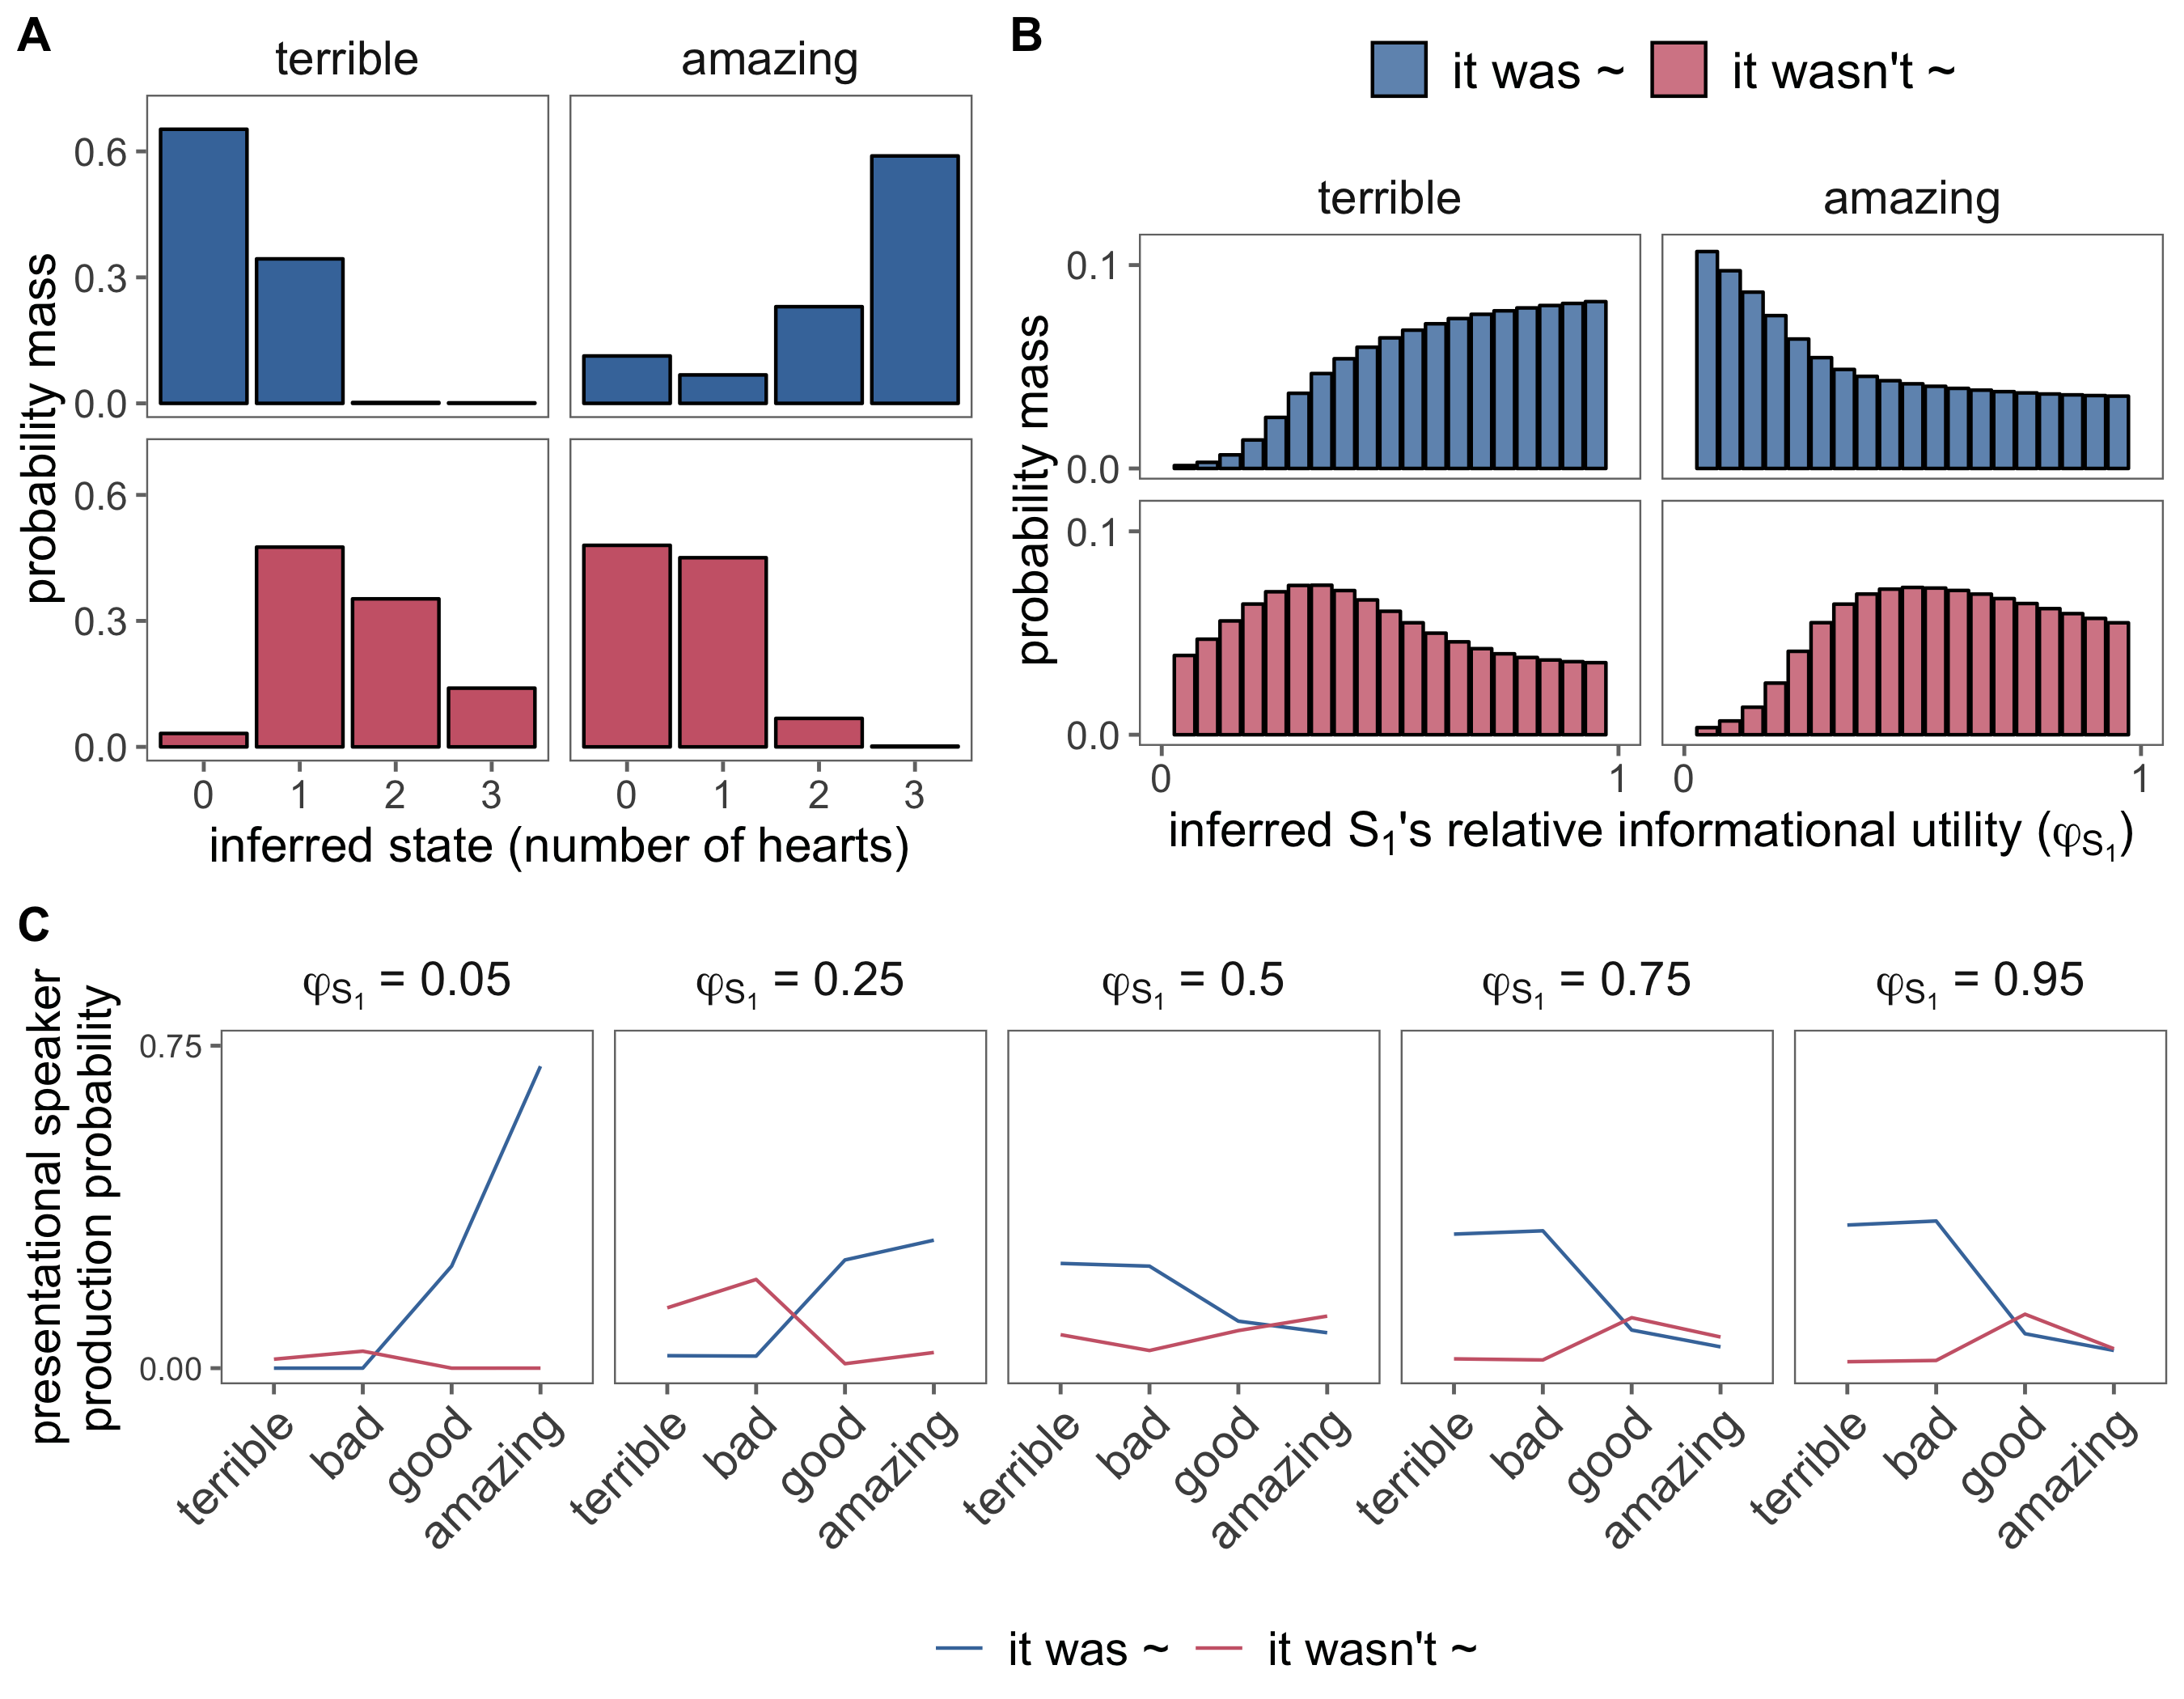
\includegraphics[width=0.9\linewidth]{/Users/ejyoon/Documents/Documents/Research/dissertation/index/chapter_child_rmds/ch2_modeling_polite/files/L1_inferences_wS2pres} 

}

\caption{Model behavior. Listener inferences about the true state (e.g., the rating truly deserved by the poem; A) and the speaker's utility weighting ($\phi_{S_1}$ or how informational vs. social the speaker is, where $\phi_{S_1}$ = 0 is fully social, and $\phi_{S_1}$ = 1 is fully informational; B) as a function of the utterance heard (facets). C: Purely self-presentational speaker production behavior as a function of the kind of speaker they wish to present themselves as (facets; relatively more informational, e.g., $\phi_{S_1}$ = 0.05, vs. social as represented, e.g., $\phi_{S_1}$ = 0.95).}\label{fig:L1inferences}
\end{figure}
\section{Model predictions}\label{model-predictions}

The pragmatic listener model \(L_1\) draws complex inferences about both
the true state of the world (Fig.~\ref{fig:L1inferences}A) and the
speaker's goals (Fig.~\ref{fig:L1inferences}B). Upon hearing
\emph{{[}Your poem{]} was terrible} (Fig.~\ref{fig:L1inferences}A
and~\ref{fig:L1inferences}B top-left), the listener infers the poem is
probably truly terrible (i.e., worthy of zero hearts) and that the
speaker has strong informational goals. \emph{It was amazing} is more
ambiguous (Figure~\ref{fig:L1inferences}A and ~\ref{fig:L1inferences}B
top-right): The poem could indeed be worthy of three hearts, but it is
also plausible the speaker had strong social goals and the poem was
mediocre. Negation makes the meanings less precise and introduces more
uncertainty into the inference about the state: A listener who hears
\emph{It wasn't amazing} sees it as a relatively kind way of saying that
the poem was quite bad (0 or 1 hearts), inferring a balance of social
and informational goals for the speaker (Figure~\ref{fig:L1inferences}A
and ~\ref{fig:L1inferences}B bottom-right). \emph{It wasn't terrible} is
the most open-ended, leaving open the possibility that the poem was
worthy of 0 hearts (i.e., \emph{it was terrible}) but conveying to the
listener that the speaker cares about both informational and social
goals, with a slight preference of towards being social
(Figure~\ref{fig:L1inferences}A and ~\ref{fig:L1inferences}B
bottom-left).

The self-presentational utility guides the speaker \(S_2\) to care about
how she will be viewed in the eyes of the listener \(L_1\)
(Figure~\ref{fig:L1inferences}C). If the speaker wants to present
herself as someone who is socially-minded (e.g., informational mixture
or \(\phi_{S_1}\) of 0.05), she should produce direct, positive
utterances (e.g., \emph{amazing}). The best way to appear honest (e.g.,
informational mixture of 0.95) is to say direct, negative utterances
(e.g., \emph{terrible}). The desire to appear as someone concerned with
telling the truth while also caring about the listener's feelings (e.g.,
\(\phi_{S_1}\) of 0.25) leads the speaker to produce indirect utterances
(e.g., \emph{not terrible}). Such indirect speech acts are sufficiently
open-ended to include the possibility that the poem was good, but the
avoidance of a more direct utterance (e.g., \emph{good}) provides the
listener with a way to recover the true state (e.g., the poem was
mediocre) by way of reasoning that the speaker cares about his feelings
by not saying the blunt truth.

\section{Experiment: Speaker production
task}\label{experiment-speaker-production-task}

We made a direct, fully pre-registered test of our speaker production
model and its performance in comparison to a range of alternative
models, by instantiating our running example in an online experiment.
\begin{figure}[!h]

{\centering 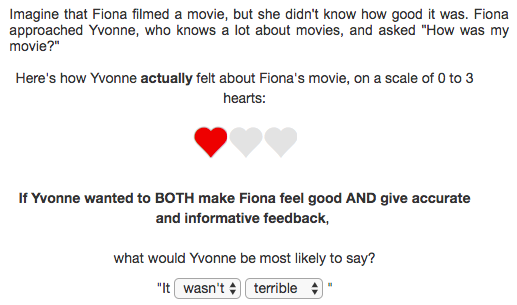
\includegraphics[width=0.9\linewidth]{/Users/ejyoon/Documents/Documents/Research/dissertation/index/chapter_child_rmds/ch2_modeling_polite/files/screenshot} 

}

\caption{Example of a trial in the speaker production task.}\label{fig:screenshot}
\end{figure}
\subsection{Participants}\label{participants}

202 participants with IP addresses in the United States were recruited
on Amazon's Mechanical Turk.

\subsection{Design and Methods}\label{design-and-methods}

Participants read scenarios with information on the speaker's feelings
toward some performance or product (e.g., a poem recital; \emph{true
state}), on a scale from zero to three hearts (e.g., one out of three
hearts). For example, one trial read: \emph{Imagine that Bob gave a poem
recital, but he didn't know how good it was. Bob approached Ann, who
knows a lot about poems, and asked} ``How was my poem?'' Additionally,
we manipulated the speaker's goals across trials: to be
\emph{informative} (``give accurate and informative feedback''); to be
\emph{kind} (``make the listener feel good''); or to be \emph{both}
informative and kind simultaneously. We hypothesized that each of the
three experimentally-induced goals would induce a different tradeoff
between social and informational utilities in our model, as well as
modulating the self-presentational component. In a single trial, each
scenario was followed by a question asking for the most likely produced
utterance by Ann. Participants selected one of eight possible
utterances, by choosing between \emph{It was} vs. \emph{It wasn't} and
then among \emph{terrible}, \emph{bad}, \emph{good}, and \emph{amazing.}

Each participant read twelve scenarios, depicting every possible
combination of the three goals and four states. The order of context
items was randomized, and there were a maximum of two repeats of each
context item per participant. Each scenario was followed by a question
that read, ``If Ann wanted to make Bob feel good but not necessarily
give informative feedback (or to give accurate and informative feedback
but not necessarily make Bob feel good, or BOTH make Bob feel good AND
give accurate and informative feedback), what would Ann be most likely
to say?'' Participants indicated their answer by choosing one of the
options on the two dropdown menus, side-by-side, one for choosing
between \emph{It was} vs. \emph{It wasn't} and the other for choosing
among \emph{terrible}, \emph{bad}, \emph{good}, and \emph{amazing.}

\subsection{Behavioral results}\label{behavioral-results}
\begin{figure}[!t]

{\centering 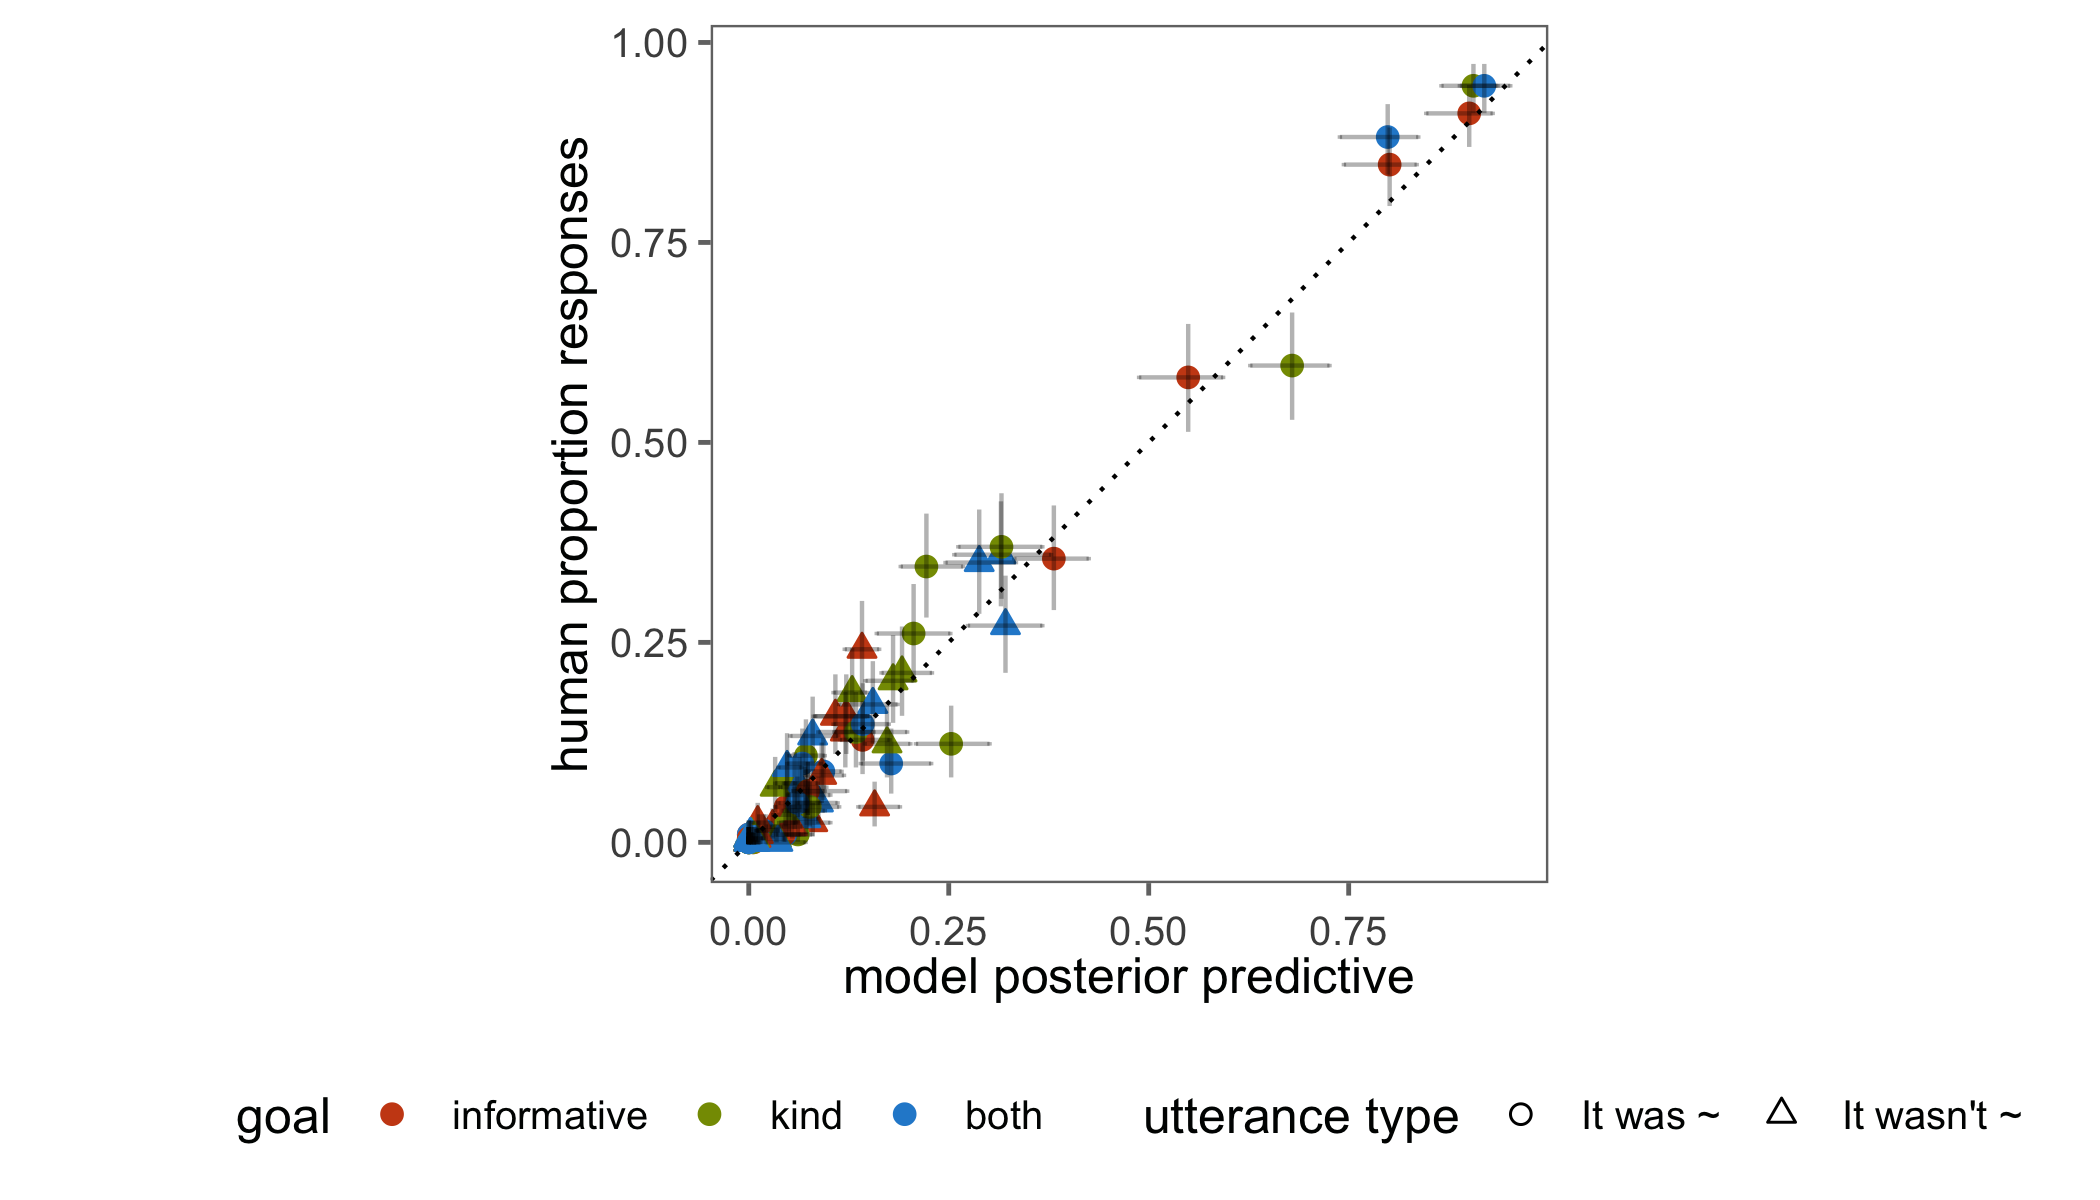
\includegraphics[width=0.9\linewidth]{/Users/ejyoon/Documents/Documents/Research/dissertation/index/chapter_child_rmds/ch2_modeling_polite/files/speaker_production_cor} 

}

\caption{Full distribution of human responses vs. model predictions. Error bars represent 95\% confidence intervals for the data (vertical) and 95\% highest density intervals for the model (horizontal).}\label{fig:variance}
\end{figure}
Our primary behavioral hypothesis was that speakers describing bad
states (e.g., poem deserving 0 hearts) with goals to be both informative
and kind would produce more indirect, negative utterances (e.g.,
\emph{It wasn't terrible}). Such indirect speech acts both save the
listener's face and provide some information about the true state, and
thus, are what a socially-conscious speaker would say
(Figure~\ref{fig:L1inferences}). This prediction was confirmed, as a
Bayesian mixed-effects model predicts more negation as a function of
true state and goal via an interaction: A speaker with both goals to be
informative and kind produced more negation in worse states compared to
a speaker with only the goal to be informative (\emph{M} = -1.33,
{[}-1.69, -0.98{]}) and goal to be kind (\emph{M} = -0.5, {[}-0.92,
-0.07{]}). Rather than eschewing one of their goals to increase utility
along a single dimension, participants chose utterances that jointly
satisfied their conflicting goals by producing indirect speech.
\begin{figure}[!t]

{\centering 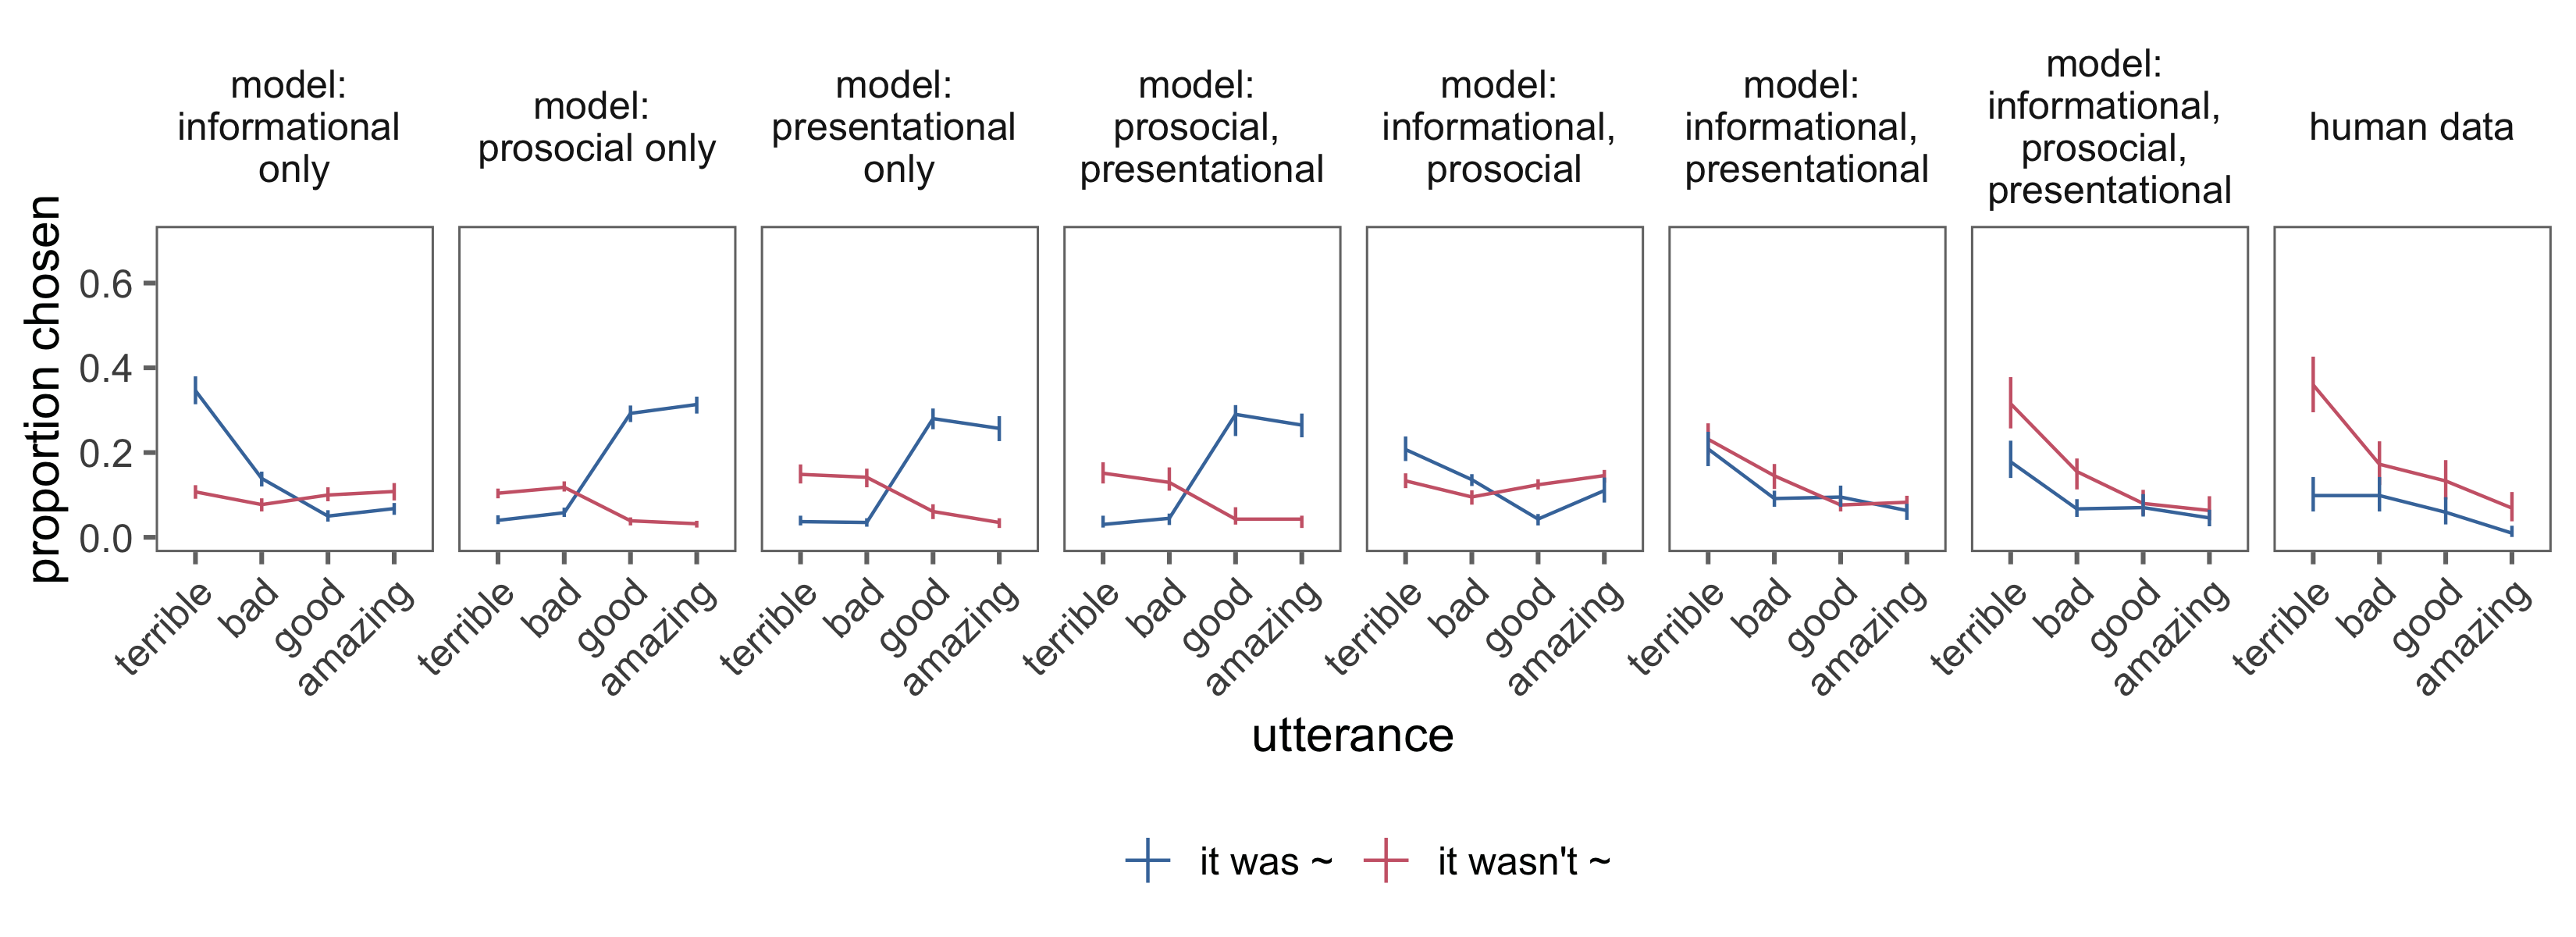
\includegraphics[width=0.9\linewidth]{/Users/ejyoon/Documents/Documents/Research/dissertation/index/chapter_child_rmds/ch2_modeling_polite/files/model_comparisons} 

}

\caption{Comparison of predictions for proportion of utterances chosen by pragmatic speaker from possible model variants (left) and human data (rightmost) for average proportion of negation produced among all utterances, given true state of 0 heart (on a scale of 0 to 3) and speaker with both goals to be informative and kind. Gray dotted line indicates chance level at 12.5\%.}\label{fig:comparison}
\end{figure}
\begin{table}[tbp]
\begin{center}
\begin{threeparttable}
\caption{\label{tab:comparisonTable}Comparison of variance explained for each model variant and log Bayes Factors quantifying evidence in favor of alternative model in comparison.}
\begin{tabular}{lll}
\toprule
model & \multicolumn{1}{c}{variance 
explained} & \multicolumn{1}{c}{log BF}\\
\midrule
informational, 
social, 
presentational & 0.97 & --\\
informational, 
presentational & 0.96 & -11.14\\
informational, 
social & 0.92 & -25.06\\
social, 
presentational & 0.23 & -864\\
presentational 
only & 0.23 & -873.83\\
social only & 0.22 & -885.52\\
informational 
only & 0.83 & -274.89\\
\bottomrule
\end{tabular}
\end{threeparttable}
\end{center}
\end{table}
\subsection{Model results}\label{model-results}

The model parameters (softmax parameters and each goal condition's
utility weights) can be inferred from the behavioral data using Bayesian
data analysis (M. D. Lee \& Wagenmakers, 2014). To approximate the
literal meanings (i.e., the semantics) of the words as interpreted by
the literal listener \(L_0\), we obtained literal meaning judgments from
an independent group of participants (See Supplmentary Materials:
Literal semantic task section). The posterior predictions from the the
three-utility polite speaker model (informational, social,
presentational) showed a very strong fit to participants' actual
utterance choices (\(r^2\)(96) = 0.971281; Figure~\ref{fig:variance}).
We compared these to six model variants containing subsets of the three
utilities in the full model. Both the variance explained and marginal
likelihood of the observed data were the highest for the full model
(Table~\ref{tab:comparisonTable}). Only the full model captured
participants' preference for negation when the speaker wanted to be
informative and kind about truly bad states, as hypothesized
(Figure~\ref{fig:comparison}). In sum, the full set of informational,
social, and presentational were required to fully explain participants'
utterance choices.
\begin{table}[tbp]
\begin{center}
\begin{threeparttable}
\caption{\label{tab:phi}Inferred phi parameters from all model variants with more than one utility.}
\begin{tabular}{llllll}
\toprule
model (utilities) & \multicolumn{1}{c}{goal} & \multicolumn{1}{c}{$\phi_{inf}$} & \multicolumn{1}{c}{$\phi_{soc}$} & \multicolumn{1}{c}{$\phi_{pres}$} & \multicolumn{1}{c}{$\phi_{S_1}$}\\
\midrule
informational, social, presentational & both & 0.36 & 0.11 & 0.54 & 0.36\\
informational, social, presentational & informative & 0.36 & 0.02 & 0.62 & 0.49\\
informational, social, presentational & social & 0.25 & 0.31 & 0.44 & 0.37\\
informational, presentational & both & 0.64 & -- & 0.36 & 0.17\\
informational, presentational & informative & 0.77 & -- & 0.23 & 0.33\\
informational, presentational & social & 0.66 & -- & 0.34 & 0.04\\
informational, social & both & 0.54 & 0.46 & -- & --\\
informational, social & informative & 0.82 & 0.18 & -- & --\\
informational, social & social & 0.39 & 0.61 & -- & --\\
social, presentational & both & -- & 0.38 & 0.62 & 0.55\\
social, presentational & informative & -- & 0.35 & 0.65 & 0.75\\
social, presentational & social & -- & 0.48 & 0.52 & 0.66\\
\bottomrule
\end{tabular}
\end{threeparttable}
\end{center}
\end{table}
The utility weights inferred for the three-utility model (Table
\ref{tab:phi}) provide additional insight into how polite language use
operates in our experimental context and possibly beyond: \emph{Being
kind} (``social'') requires not only weights on social and
presentational utilities but equal weights on all three utilities,
indicating that informativity is a part of language use even when it is
explicitly not the goal. \emph{Being informative} (``informative'')
pushes the weight on social utility (\(\phi_{soc}\)) close to zero, but
the weight on \emph{appearing kind} (\(\phi_{pres}\)) stays high,
suggesting that speakers are expected to manage their own face even when
they are not considering others'. \emph{Kind and informative} (``both'')
speakers emphasize informativity slightly more than kindness. In all
cases, however, the presentational utilities have greatest weight,
suggesting that managing the listener's inferences about oneself was
integral to participants' decisions in the context of our communicative
task. Overall then, our condition manipulation altered the balance
between these weights, but all utilities played a role in all
conditions.

\section{Discussion}\label{discussion}

Politeness is puzzling from an information-theoretic perspective.
Incorporating social motivations adds a level of explanation, but so far
such intuitions and observations have resisted both formalization and
precise testing. We present a utility-theoretic model of language use
that captures the interplay between competing informational, social, and
presentational goals, and provide preregistered experimental evidence
that confirmed its ability to capture human judgments, unlike comparison
models with only a subset of the full utility structure.

To estimate precisely choice behavior in the experiment, it was required
to abstract away from natural interactions in a number of ways. Human
speakers have access to a potentially infinite set of utterances to
select from in order to manage the three-utility tradeoff (\emph{It's
hard to write a good poem}, \emph{That metaphor in the second stanza was
so relatable!}). In theory, each utterance will have strengths and
weaknesses relative to the speaker's goals, though computation in an
unbounded model presents technical challenges (perhaps paralleling the
difficulty human speakers feel in finding the right thing to say in a
difficult situation; see N. D. Goodman \& Frank, 2016a).

For a socially-conscious speaker, managing listeners' inferences is a
fundamental task. Our work extends previous models of language beyond
standard informational utilities to address social and
self-presentational concerns. Further, our model builds upon the theory
of politeness as face management (P. Brown \& Levinson, 1987) and takes
a step towards understanding the complex set of social concerns involved
in face management. Our approach can provide insight into a wide range
of social behaviors beyond speech by considering utility-driven
inferences in a social context (Baker, Jara-Ettinger, Saxe, \&
Tenenbaum, 2017; Hamlin, Ullman, Tenenbaum, Goodman, \& Baker, 2013)
where agents need to take into account concerns about both self and
others.

Previous game-theoretic analyses of politeness have either required some
social cost to an utterance (e.g., by reducing one's social status or
incurring social debt to one's conversational partner; Van Rooy, 2003)
or a separately-motivated notion of plausible deniability (Pinker et
al., 2008). The kind of utterance cost for the first type of account
would necessarily involve higher-order reasoning about other agents, and
may be able to be defined in terms of the more basic social and
self-presentational goals we formalize here. A separate notion of
plausible deniability may not be needed to explain most politeness
behavior, either. Maintaining plausible deniability is in one's own
self-interest (e.g., due to controversial viewpoints or covert
deception) and goes against the interests of the addressee; some amount
of utility dis-alignment is presumed by these accounts. Politeness
behavior appears present even in the absence of obvious conflict,
however: In fact, you might be even more motivated to be polite to
someone whose utilities are more aligned with yours (e.g., a friend). In
our work here, we show that such behaviors can in fact arise from purely
cooperative goals (P. Brown \& Levinson, 1987), though in cases of
genuine conflict, plausible deniability likely plays a more central role
in communication.

Utility weights and value functions in our model could provide a
framework for a quantitative understanding of systematic cross-cultural
differences in what counts as polite. Cross-cultural differences in
politeness could be a product of different weightings within the same
utility structure. Alternatively, culture could affect the value
function \(V\) that maps states of the world onto subjective values for
the listener (e.g., the mapping from states to utilities may be
nonlinear and involve reasoning about the future). Our formal modeling
approach with systematic behavior measurements provides an avenue
towards understanding the vast range of politeness practices found
across languages.

Politeness is only one of the ways language use deviates from purely
informational transmission. We flirt, insult, boast, and empathize by
balancing informative transmissions with goals to affect others'
feelings or present particular views of ourselves. Our work shows how
social and self-presentational motives are integrated with informational
concerns more generally, opening up the possibility for a broader theory
of social language. In addition, a formal account of politeness moves us
closer to courteous computation -- to machines that can talk with tact.

\chapter[Children understand social goals behind polite
requests]{\texorpdfstring{Children understand social goals behind polite
requests\footnote{This chapter is submitted and currently under review
  for the 41st Annual Meeting of the Cognitive Science Society, and is
  joint work with Michael C. Frank.}}{Children understand social goals behind polite requests}}\label{children-understand-social-goals-behind-polite-requests}

\chaptermark{Children's understanding of polite requests}

In the last chapter, I examined adults' understanding of polite speech
based on goal tradeoffs. What do children understand about polite
speech? Looking at children's polite speech comprehension can help
examine children's pragmatic understanding more generally, and can be
informative for caregivers who want to teach children what it means to
be polite. Even though children start to produce polite speech from
early on, there is little known about whether they understand intentions
behind polite language. In this Chapter, I show that by 3 years,
English-speaking preschool children understand that it is more polite
and nicer (and less rude and mean) to use politeness markers such as
"please" when making requests, and by 4 years, they understand that the
use of these politeness markers indicates that the speaker is more
socially likeable and is more likely to gain compliance from their
conversational partners. This work can help lay the foundation for
future work on children's understanding of polite speech and pragmatic
development more generally.

\section{Introduction}\label{introduction-2}

We use and hear polite speech on a daily basis: polite utterances range
from simple words of apology (``sorry'') or gratitude (``thanks'') to
compliments (``I love your dress!'') and requests (``Can you please open
the window?''). Yet polite utterances are seemingly inefficient and even
misinformative: speakers say ``Can you please \ldots{}'' when it should
suffice to say, ``Open the window.'' These facts are a mystery for
frameworks which describe communication in terms of efficient
information transfer (e.g., Bühler, 1934; N. D. Goodman \& Stuhlmüller,
2013; Shannon, 1948): If language is a tool for transferring
information, speakers should be as efficient as possible in their
communication to prioritize informativity. Nonetheless, everyday
politeness is ubiquitous in everyday language use, and adults tend to
use strategies to be polite even while arguing (T. Holtgraves, 1997).

So why do people speak politely? Linguistic theories assume that
people's utterance choices are motivated by social concerns, framed as
either maxims (Leech, 1983), social norms (Ide, 1989), or listener's
and/or speaker's public identity (\emph{face}; P. Brown \& Levinson,
1987). For example, P. Brown \& Levinson (1987)'s theory predicts that
if a speaker's intended meaning contains a threat to the listener's face
or self-image, the speaker's utterance will be less direct and less
informative. For example, if a speaker considered that saying ``Open the
window'' will give the impression that she is in a position to give
orders to the listener, she could instead say ``Can you please open the
window?'', using a more indirect form of request to give the other
person a sense of autonomy or freedom from imposition (H. H. Clark \&
Schunk, 1980). Thus, while it may hinder the goal of efficient
information transfer, using polite speech can help the speaker save the
listener's face while simultaneously communicating her own positive
social goals (Erica J. Yoon, Tessler, Goodman, \& Frank, 2017).

Do children speak politely, and if so, what do they understand about
polite speech? Previous research shows that children begin producing
polite speech early on; They produce ``please'' at 2.5 years (Read \&
Cherry, 1978), and request forms increase in their variety and frequency
with age (E. Bates, 1976; E. Bates \& Silvern, 1977; Bock \& Hornsby,
1981; Ervin-Tripp, 1982; Nippold et al., 1982). Young children learn to
produce different forms of requests depending on context: For example,
by three years children are able to vary their utterances based on
whether they are instructed to ``tell'' versus ``ask'' an addressee to
given them a puzzle piece (Bock \& Hornsby, 1981). And even at two
years, children are able to modify their requests to make them more
polite (``ask in the nicest way possible''; E. Bates \& Silvern, 1977).
Hence, children's production of polite speech seems to parallel adult
speakers' desires to produce utterances with appropriate levels of
face-saving.

While children appear to produce polite speech from an early age, less
is known about whether they \emph{understand} polite speech. Examining
children's comprehension of polite speech is important for a number of
reasons. First, children's polite speech understanding can reveal their
inferential abilities underlying more general pragmatic understanding:
going beyond what was literally said to infer what was intended. For
example, children need to understand that, in saying ``can you open the
window?'' the speaker does not literally question the listener's ability
to open the window but rather wants to make a polite request. Thus,
understanding what children comprehend about polite speech can help see
how children are able to infer speaker's intentions behind utterances.

Second, understanding polite speech can have practical implications for
education, as caregivers often care about teaching their children to be
more polite. Indeed, from very early on, parents teach children to
follow normative rituals to say ``please'', ``thank you'', ``hello'' and
``good-bye'' (Gleason et al., 1984). It can be enlightening to know
whether and when children understand positive implications of following
these norms.

Third, examining children's \emph{comprehension} of polite speech as
compared to their \emph{production} is meaningful, in that children's
comprehension can reveal more abstract representations and inferences
about language than their productivity (e.g., Fisher, 2002): Children's
ability to say ``please'' early on does not necessarily indicate that
they understand saying ``please'' is more polite, nicer and socially
apt, as children may simply obey or imitate what their caregivers tell
them to say without understanding its meaning.

Research on children's comprehension of polite speech has received less
focus than research on their production of polite speech. Moreover, the
few studies that did examine children's understanding of polite speech
have been largely inconclusive. Though there was some initial evidence
to suggest that producing a request with ``please'' is judged to be
polite by three years of age (E. Bates, 1976; E. Bates \& Silvern,
1977), in a later study, the judgment of ``please'' as being polite was
only replicated starting at five years of age, but not younger (Nippold
et al., 1982). These initial studies also lacked statistical tests to
assess each age group's performance, and did not systematically
manipulate cues other than linguistic markers (e.g., prosody or facial
expressions).

In addition to children's recognition of politeness markers, there are
also many open questions about their abilities to recognize the
intentions underlying polite speech. For example, do children know that
the word ``polite'' should be associated with politeness rules people
abide by (e.g., saying ``please'')? Relatedly, do children recognize
polite speech as being positively valenced, such that they think it is
better and nicer to say polite things? Do children understand the social
implications of speaking politely? For example, polite people may be
more likely to get their wishes granted (``I will pour him more water
because he was nice'') and may be better social play partners compared
to those who are impolite. Finally, what cues to politeness do children
recognize? Do they recognize linguistic politeness markers such as
``please,'' or ``can you,'' or both? Or do they rely on prosodic cues
that make utterances sound more respectful, or on facial expressions
that make a person look kind?

In this current work, we sought to answer these questions, and test what
2- to 4-year-old children understand about requests using politeness
markers. Across three experiments, we presented stories about speakers
who decided to speak politely (e.g., ``Please pour me more water'') or
impolitely (``Pour me more water'') and asked child participants to make
judgments between the two speakers. We examined in each experiment
whether: (1) children are able to reason about speakers using polite
speech as being relatively more ``polite'' and ``nice'' and less
``rude'' or ``mean'' than speakers not using polite speech; (2) they can
reason about social implications of using polite speech (e.g.,
politeness as a sign of a nice play partner, or greater likelihood of
compliance from the addressee); and (3) they show improvement with age
for these lines of reasoning. We also examined whether children need
additional cues to politeness such as facial expressions (Expt 1) or
prosodic cues (Expt 2), or they can make use of linguistic politeness
markers alone (Expt 3) to make appropriate inferences about speakers.

\section{Experiment 1}\label{experiment-1}

In Experiment 1, we tested whether 3- to 4-year-old children were able
to understand the implications of using simple politeness markers, based
on linguistic cues of interest (whether the speaker says ``please,''
``can you'') and other cues (facial expressions and prosodic cues) that
make polite speech more salient and naturalistic.

\subsection{Methods}\label{methods}

\subsubsection{Participants}\label{participants-1}

3-year-old (\(n=\) 20; 12 F, \(M_{age}\) = 3.61 years, \(SD_{age}\) =
0.22) and 4-year-old children (\(n=\) 18; 6 F, \(M_{age}\) = 4.38 years,
\(SD_{age}\) = 0.25) were recruited from a local preschool. An
additional 3 children were tested but excluded due to failure on the
practice questions (\(n=\) 2) or completion of fewer than half of the
test trials (\(n=\) 1).

\subsubsection{Stimuli and design}\label{stimuli-and-design}

We designed a picture book with twelve stories in which a protagonist is
approached by two speakers, one of whom makes a request by producing an
utterance with a politeness marker (e.g., ``Please pour me more
water''), and the other produces an utterance without (``Pour me more
water''). There were three types of politeness marker that could be
used: ``please'' (as in ``Please pour me more water''), ``can you''
(``Can you pour me more water''), and ``can you please'' (``Can you
please pour me more water'').

We designed six question types to ask participants following the
presentation of the stories: four \emph{speaker attribute} questions
(\emph{polite}: ``Which one was more polite?''; \emph{rude}: ``Which one
was more rude?''; \emph{nice}: ``Which one was nicer?''; \emph{mean}:
``Which one was meaner?'') and two \emph{social implication} questions
(\emph{play partner}: ``Which one would you rather play with?'';
\emph{compliance}: ``Which one will {[}get what they want{]}?''). Each
participant would be asked one of the four speaker attribute questions,
followed by one of the two social implication questions.

In Experiment 1, all utterances were produced live by the experimeter,
with appropriate proodic cues and facial expressions for each request:
Utterances with politeness markers were produced by kind voice and
facial expression, whereas utterances lacking politeness marker were
produced with angry voice and facial cues.

\subsubsection{Procedure}\label{procedure}

The experimenter presented to the child a storybook with a total of
thirteen stories about different characters. In the \emph{practice}
phase, the child heard a story with one clearly mean character
(\emph{Drew kicked Carol}) and one clearly nice character (\emph{Graham
gave Carol a gift}). After a reminder of what each character did, the
experimenter asked the participant: \emph{Which one was being meaner?}
and \emph{Which one was being nicer?} If the child answered the question
wrong the first time, the experimenter read the story one more time,
saying, ``Let's think about the story one more time.'' Only children who
correctly answered both questions in the first or second attempt were
included in the analyses.

In the \emph{test} phase, the child heard twelve stories, in each of
which they saw one speaker who decided to speak politely (\emph{Jean
wanted more water in her cup. Jean said to Fred, ``Please pour me more
water''}) and another speaker who spoke impolitely (\emph{Suzy also
wanted more water in her cup. Suzy said to Fred, ``Pour me more
water.''}). After a reminder about what each speaker said, the child was
asked a total of two questions. For the first question, the experimenter
asked one out of four possible questions for speaker attribute: ``Which
one was being more polite {[}more rude/nicer/meaner{]}?'' For the
second, social implication question, the experimenter either asked about
play partner (\emph{Which one would you rather play with?}) or
likelihood of compliance (e.g., \emph{Which one will Fred give water
to?}). The order of story types and question types was counterbalanced.

\subsection{Results and Discussion}\label{results-and-discussion}

\newpage

\blandscape
\begin{figure*}[p]

{\centering 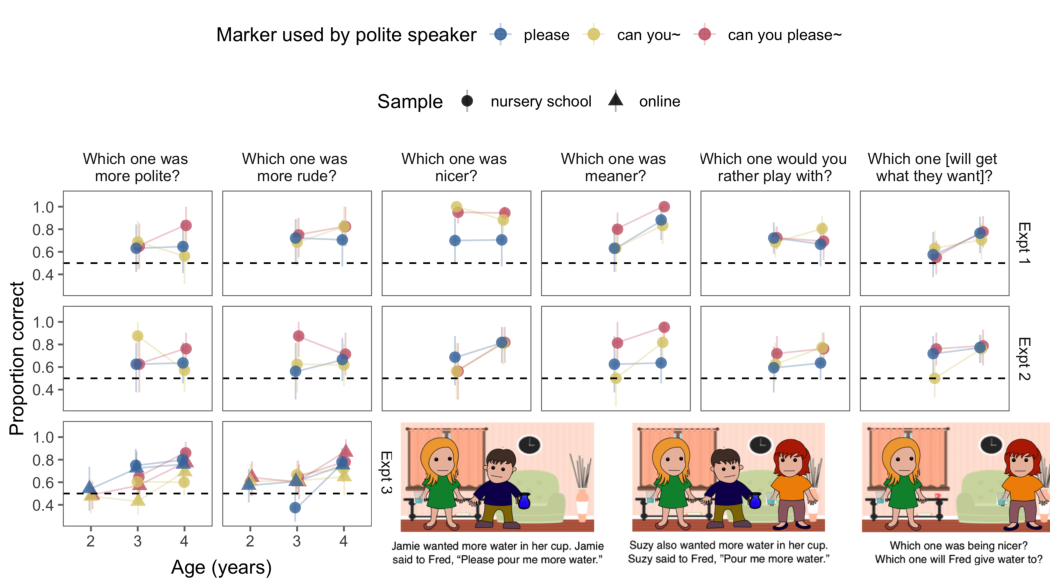
\includegraphics[width=0.9\linewidth]{erica_yoon_dissertation_files/figure-latex/figResultsPlacement-1} 

}

\caption{Bottom right: Story example. Top, left: Results. Proportion of correct responses to questions comparing between a speaker who used a politeness marker (where blue indicates "please", yellow "can you", and red "can you please") versus a speaker who did not. Data are binned into one-year age groups. Each row represents data from a different Experiment. Columns represent different questions asked. Dashed line represents chance level (i.e., if participant were guessing at random).}\label{fig:figResultsPlacement}
\end{figure*}
\elandscape

We looked at the proportion of correct responses to various questions
comparing speakers who used a politeness marker and spoke kindly, and
speakers who did not use a politeness marker and spoke meanly
(Figure~\ref{fig:figResultsPlacement}, first row). A mixed-effects
logistic regression predicting accuracy based on age, question type and
politeness marker type\footnote{for Experiments 1 and 2, we use this
  model structure with a maximal random effect structure that converges:
  \texttt{accuracy\ \textasciitilde{}\ age\ x\ question\ type\ x\ politeness\ marker\ type\ +\ (1\ \textbar{}\ item)},
  where age is continuous, centered and scaled. All categorical
  variables were deviation coded, with specified contrasts of interest
  for the question type. Significance was calculated using the standard
  normal approximation to the \(t\) distribution (Barr, Levy, Scheepers,
  \& Tily, 2013a).} showed there was an improvement with age (\(\beta\)
= 0.2, \(p =\) 0.026). The regression model also revealed that children
seemed to find some question types easier than others: Responses to
\emph{nice} and \emph{mean} questions were more accurate than to
\emph{polite} and \emph{rude} questions (\(\beta\) = 0.8, \(p =\)
0.002), whereas social implication questions (\emph{play partner} and
\emph{compliance}) were overall more difficult compared to speaker
attribute questions (\emph{polite}, \emph{rude}, \emph{nice}, and
\emph{mean}; \(\beta\) = -0.33, \(p =\) 0.006).

Looking more closely at responses for each of the question types,
children from both age groups tended to accurately answer the
\emph{polite}, \emph{nice}, \emph{mean}, \emph{rude}, and \emph{play
partner} questions overall (3-year-olds' mean accuracy range: 0.58 -
0.88; 4-year-olds' mean accuracy range: 0.68 - 0.9), indicating
correctly that the speaker who used a politeness marker was more polite
and nicer, and less mean and rude, and was likely a better play partner.
For the \emph{compliance} question, 4-year-olds overall answered
correctly that the speaker who used politeness marker will likely get
what they want from the listener (\(M_{4y}\) = 0.75, \(p\) \textless{}
.01), but 3-year-olds did not perform above chance (\(M_{3y}\) = 0.58).
As for the different politeness marker types, both age groups overall
tended to give correct answers based on all three markers, but
especially ``can you please'' (3-year-olds: \(M_{please}\) = 0.66,
\(M_{can you}\) = 0.72, \(M_{can you please}\) = 0.74; 4-year-olds:
\(M_{please}\) = 0.73, \(M_{can you}\) = 0.77, \(M_{can you please}\) =
0.84).

In sum, in this first experiment, we saw preliminary evidence that
children pay attention to some cues to politeness and are able to use
these cues to infer whether speakers are relatively polite, rude, nice
or mean, and whether speakers are good play partners and are likely to
get what they wanted from their addressees. 4-year-olds answered
questions accurately more often compared to 3-year-olds, especially for
the question about addressee's compliance with the speaker's request. In
general, however, both age groups tended to be accurate when all the
possible cues were used to signal that one speaker was polite (used
``can you please'', spoke with a kind tone and face) and the other
speaker wasn't (did not use a politeness marker, spoke with an angry
tone and face).

There were a number of remaining issues from Experiment 1. Children may
not have used the linguistic politeness markers (e.g., ``please'') per
se, and rather prosodic and facial cues that accompany these markers.
That is, children may have relied on the speaker's kind voice and face
rather than their use of ``please'' to evaluate their niceness or
likeability as a play partner. Similarly, greater accuracy for some
questions over others (e.g., \emph{nice} \textgreater{} \emph{polite})
may have been due to greater association between some of the words and
prosodic and facial cues (e.g., a kind face may be seen to signal
niceness more than politeness), not due to greater understanding for
those words or concepts. Another concern is that the experimenter was
aware of the manipulations (i.e., they knew which speaker was supposed
to be ``polite'') and thus could have affected the presentation of these
speakers in ways that are not consistent across all participants. In our
next two experiments, we sought to remove these potential confounds.

\section{Experiment 2}\label{experiment-2}

In Experiment 1, we saw initial evidence that children can use some
combinations of linguistic, prosodic, and facial cues to politeness. In
Experiment 2, we examined whether children can make similar judgments
using linguistic and prosodic cues only, without facial expressions. For
this, we conducted a preregistered experiment where we used pre-recorded
voiceovers to present speaker utterances, so that (1) we could look at
children's judgments based on linguistic markers and prosodic cues only,
and (2) we could remove the role of the experimenter in presentation of
these utterances.

\subsection{Methods}\label{methods-1}

\subsubsection{Participants}\label{participants-2}

3-year-old (\(n=\) 16; 8 F, \(M_{age}\) = 3.56 years, \(SD_{age}\) =
0.29) and 4-year-old children (\(n=\) 22; 13 F, \(M_{age}\) = 4.5 years,
\(SD_{age}\) = 0.32) were recruited from a local preschool. An
additional 5 children were tested but excluded due to failure on the
practice questions.

\subsubsection{Stimuli and design}\label{stimuli-and-design-1}

The design was identical to Experiment 1. Stimuli were the same as
Experiment 1 except two changes: (1) Instead of a picture book, we
presented the stories on a tablet; (2) the speakers' utterances were now
presented as recorded voiceovers. The voiceovers were recorded by native
English speakers, and contained prosodic cues that matched the
presence/absence of a politeness marker (e.g., ``Please pour me more
water'' was recorded with a kind voice and ``pour me more water'' with
an angry voice).

\subsubsection{Procedure}\label{procedure-1}

The procedure was identical to Experiment 1, except for the following
change: The participants now had to tap on a speaker on tablet in order
either to hear them speak, or to choose an answer to the questions
asked.

\subsection{Results and Discussion}\label{results-and-discussion-1}

Overall we saw similar patterns of results in Experiment 2
(Figure~\ref{fig:figResultsPlacement}, second row) compared to Exp. 1. A
mixed-effects logistic regression predicting accuracy based on age,
question type and politeness marker type showed that accuracy improved
with age (\(\beta\) = 0.25, \(p =\) 0.002), and children made accurate
judgments more often when the politeness marker was ``can you please''
than when the marker was ``please'' or ``can you'' (\(\beta\) = 0.33,
\(p =\) 0.019). There was no main effect of question type, but there was
an interaction between age and question type such that performance for
\emph{nice} and \emph{mean} questions saw greater improvement with age
than for \emph{polite} and \emph{rude} questions (\(\beta\) = 0.57,
\(p =\) 0.011).

For children's responses to different question types, 3-year-olds'
accuracy did not differ from chance level for \emph{nice}, \emph{mean},
and \emph{play partner} questions, but their means numerically exceeded
50\% for all question types, and 4-year-olds accurately answered
questions of all types (3-year-olds' mean accuracy range: 0.6 - 0.88;
4-year-olds' mean accuracy range: 0.66 - 0.9). For politeness marker
types, 3-year-olds' performance did not differ from chance for
``please'' and ``can you'', but both age groups tended to answer
questions about different politeness markers accurately overall
(3-year-olds: \(M_{please}\) = 0.63, \(M_{can you}\) = 0.61,
\(M_{can you please}\) = 0.72; 4-year-olds: \(M_{please}\) = 0.7,
\(M_{can you}\) = 0.72, \(M_{can you please}\) = 0.8).

In sum, across Experiments 1 and 2, we saw that children tend to make
accurate judgments about speakers given their use of politeness markers,
especially ``can you please,'' together with prosodic cues, and children
get better with age in their use of politeness cues to respond to
questions about speaker attributes and social implications.

\section{Experiment 3}\label{experiment-3}

We conducted a third, pre-registered experiment to see whether children
are able to evaluate speakers based on linguistic markers only, without
any other supporting cues such as prosodic cues or facial expressions.

\subsection{Methods}\label{methods-2}

\subsubsection{Participants}\label{participants-3}

We recruited two samples of participants: one from the same local
nursery school as Experiments 1 and 2, and the other from Lookit
(\url{https://lookit.mit.edu/}), an online platform for child research
participation, in which parents and their children can participate
together. The nursery school sample consisted of 3-year-old (\(n=\) 24;
11 F, \(M_{age}\) = 3.65 years, \(SD_{age}\) = 0.26) and 4-year-old
children (\(n=\) 25; 13 F, \(M_{age}\) = 4.48 years, \(SD_{age}\) =
0.28). An additional 3 children were tested but excluded due to failure
on the practice questions. The online sample consisted of 2-year-old
(\(n=\) 23; 12 F, \(M_{age}\) = 2.48 years, \(SD_{age}\) = 0.29),
3-year-old (\(n=\) 31; 15 F, \(M_{age}\) = 3.59 years, \(SD_{age}\) =
0.27) and 4-year-old children (\(n=\) 27; 12 F, \(M_{age}\) = 4.46
years, \(SD_{age}\) = 0.29). An additional 28 children were tested but
excluded due to failure on the practice questions (\(n=\) 19) or
completion of fewer than half of the test trials (\(n=\) 9).

\subsubsection{Stimuli}\label{stimuli}

For the nursery school sample, stimuli were identical to Experiment 2
except that the voiceovers for all utterances had the same prosody: All
utterances ended with a rising intonation. For the online sample,
stimuli were identical to what the nursery school participants saw
except that the story narrations (other than speaker utterances) were
also pre-recorded such that parents did not need to read the stories
aloud to their children.

\subsubsection{Procedure}\label{procedure-2}

For the nursery school sample, the procedure was identical to Experiment
2. For the online sample, the procedure was similar except that parents
and children participated together at home and there was no experimenter
present. Parents accessed the webpage for the study and gave their
consent for participation, and then read instructions to proceed through
the different stories, which specifically asked the parents to not tell
their children correct answers for the questions.

\subsection{Results and Discussion}\label{results-and-discussion-2}

\subsubsection{Experiment 3}\label{experiment-3-1}

For Experiment 3, we were able to look at how children answered the
\emph{polite} and \emph{rude} questions given the same three politeness
marker types as in Experiments 1 and 2, with three age groups including
2-year-olds. (Fig. ~\ref{fig:figResultsPlacement}, third row).

A mixed-effects logistic regression controlling for the effect of
sample\footnote{Model structure:
  \texttt{accuracy\ \textasciitilde{}\ sample\ +\ age\ x\ question\ type\ x\ politeness\ marker\ type\ +\ (1\ \textbar{}\ item)}}
showed improvement with age (\(\beta\) = 0.19, \(p =\) 0.033) as well as
better performance for ``can you please'' than ``please'' and ``can
you'' together (\(\beta\) = 0.42, \(p =\) 0.002), consistent with
Experiment 2 results. Performance for ``please'' was also better than
for ``can you please'' and ``please'' together (\(\beta\) = 0.3, \(p =\)
0.027), which may be surprising given that we previously did not see the
same effect in Experiments 1 and 2. One possible explanation is that
controlling for prosodic cues in Experiment 3 actually made it
\emph{easier} to use ``please'' as a politeness cue. Because we had
stripped all the other variations, it may have made the contrast between
the presence and absence of the marker ``please'' \emph{more} salient.

Additionally, children were better with the \emph{polite} questions than
\emph{rude} overall (\(\beta\) = -0.19, \(p =\) 0.04), but especially
given ``please'' (\(\beta\) = 0.42, \(p =\) 0.002). Finally, children
showed a greater improvement with age for ``can you please'' compared to
``please'' and ``can you'' together (\(\beta\) = 0.38, \(p =\) 0.004).

\subsubsection{All experiments}\label{all-experiments}

Did children perform better given facial and/or prosodic cues, or were
linguistic politeness markers sufficient? To see any potential effect of
experiment on children's performance, we conducted an exploratory
mixed-effects logistic regression on all three experiments
together\footnote{Model structure:
  \texttt{accuracy\ \textasciitilde{}\ sample\ +\ experiment\ +\ age\ x\ question\ type\ x\ politeness\ marker\ type\ +\ (1\ \textbar{}\ item)}}.
The regression model showed no significant main effect of experiment,
suggesting that children did not perform more poorly when facial and
prosodic cues were removed, and they were able to make accurate
judgments based on linguistic cues alone. The model also showed that
children improved with increasing age (\(\beta\) = 0.33, \(p\)
\textless{} .001) and that children were more accurate with ``can you
please'' than ``please'' and ``can you'' (\(\beta\) = 0.25, \(p =\)
0.011), confirming results from each individual experiment.
Additionally, the model showed that children became better at judging
the politeness marker ``can you please'' with age (\(\beta\) = 0.73,
\(p =\) 0.005), and that children answered \emph{polite} questions
better than \emph{rude} questions about the marker ``please'' (\(\beta\)
= 0.26, \(p =\) 0.006)

\section{General Discussion}\label{general-discussion}

What do young children understand about polite speech? In three
experiments, we looked at how 2- to 4-year-old children reason about
making requests with or without simple politeness markers such as
``please'', ``can you'' and ``can you please.'' By 3 years, children pay
attention to the use of politeness markers to accurately judge whether
that speaker is relatively more polite, rude, nicer or meaner compared
to another speaker. By 4 years, children reliably infer that a speaker
who uses a politeness marker is a better play partner and more likely to
get what they want. Across all three experiments, we saw a clear
developmental trend such that children improved in their reasoning about
polite speech with increasing age. We observed no large experiment
effects as we eliminated facial and prosodic cues; instead, all these
inferences appeared to be supported by linguistic markers alone.

Even though children have been shown to produce polite speech such as
``please,'' evidence has been sparse and inconclusive for whether young
children below 5 years comprehend speaker attributes and intentions
based on polite speech. Here, we found that children are sensitive to
the use of politeness markers in speech, and are able to use these
markers to infer the speaker's attributes (e.g., niceness) by 3 years,
and consequent social implications by 4 years. These ages are closer to
the age of first reliable production of polite speech than have been
suggested by earlier work.

Children in the US are often explicitly taught and prompted to use
politeness markers such as ``please'' in their requests from early on
(e.g., ``What's the magic word?''; Gleason et al., 1984), thus they may
quickly learn to use these markers as a rule in order to get what they
want. They also might hear other remarks that pair politeness markers
with positive words (e.g., ``You should be \emph{nice} and say
\emph{please}''), which may help them learn the association between
polite speech and positive attributes. Gradually, children may recognize
more subtle social processes that are related to polite speech
production: Adults may praise and reward children who spoke politely,
and children themselves may like peers who ask for permission to play
with their toys rather than take the toys away without asking. Future
work with corpus data analysis looking at these interactions between
children and others may reveal important conversational patterns that
help children acquire social meanings of polite speech.

There are limitations to the current work that present other
opportunities for future research. Because this work looked only at the
behaviors of English-speaking children with a relatively high
socioeconomic status in the US, it is an open question how children with
different language and cultural background may develop understanding of
polite speech. Cross-cultural investigation of what markers are present
in other languages, cultures and backgrounds, as well as how those
markers are acquired, will be informative.

Also, we did not manipulate the social status of speakers or addressees.
Though not explicitly stated, the visual depiction and narration used
for the current work suggested that speakers were communicating with
their peers only. However, one key prediction from politeness theory is
that speakers will adjust their utterances based on the status of the
addressees (P. Brown \& Levinson, 1987). Indeed children adjust own
their speech based on the listener status and age: Even at two years,
children use a polite form of request (``Can I have\ldots{}'') to an
adult but an imperative form (``Give me\ldots{}'') to a peer (Shatz \&
Gelman, 1973). Thus, future work should examine how children use cues to
politeness to judge speaker intentions in different contexts, including
varied status differences between speakers and listeners.

In sum, the current work showed that young children understand
implications of using simple politeness markers in requests. A broader
understanding of the emergence of politeness may offer insights into how
children become proficient users of language across the wide range of
social situations that they encounter.

\chapter[Social cues modulate attention and memory during
cross-situational word learning]{\texorpdfstring{Social cues modulate
attention and memory during cross-situational word learning\footnote{This
  chapter is published in MacDonald, Yurovsky, \& Frank (2017) Social
  cues modulate the representations underlying cross-situational
  learning. \emph{Cognitive Psychology }, 94, 67-84.}}{Social cues modulate attention and memory during cross-situational word learning}}\label{social-cues-modulate-attention-and-memory-during-cross-situational-word-learning}

\chaptermark{Social cues modulate word learning}

In this chapter, we present a series of studies exploring adults' word
learning in the presence of social cues that disambiguate reference.
Within our broader active-social framework, these experiments
investigate how social information changes statistical word learning by
(1) providing stronger information (i.e., answers) about the target
word-object link and (2) constraining the number of potential
word-object links (i.e., hypotheses) that learners track over time.
Overall, this line of work brings together ideas from social-pragmatic
and statistical accounts of language acquisition to explore how social
cues can shape the representations that support cross-situational word
learning.

Because learners hear language in environments that contain many things
to talk about, figuring out the meaning of even the simplest word
requires making inferences under uncertainty. A cross-situational
statistical learner can aggregate across naming events to form stable
word-referent mappings, but this approach neglects an important source
of information that can reduce referential uncertainty: social cues from
speakers (e.g., eye gaze). In four large-scale experiments with adults,
we tested the effects of varying referential uncertainty in
cross-situational word learning using social cues. Social cues shifted
learners away from tracking multiple hypotheses and towards storing only
a single hypothesis (Experiments 1 and 2). Also, learners were sensitive
to graded changes in the strength of a social cue, and when it became
less reliable, they were more likely to store multiple hypotheses
(Experiment 3). Finally, learners stored fewer word-referent mappings in
the presence of a social cue even when given the opportunity to visually
inspect the objects for the same amount of time (Experiment 4). These
results suggest that the representations underlying cross-situational
word learning of concrete object labels flexibly respond to uncertainty
in the input. And when ambiguity is high, learners tend to store a
broader range of information.
\begin{figure}[!t]

{\centering 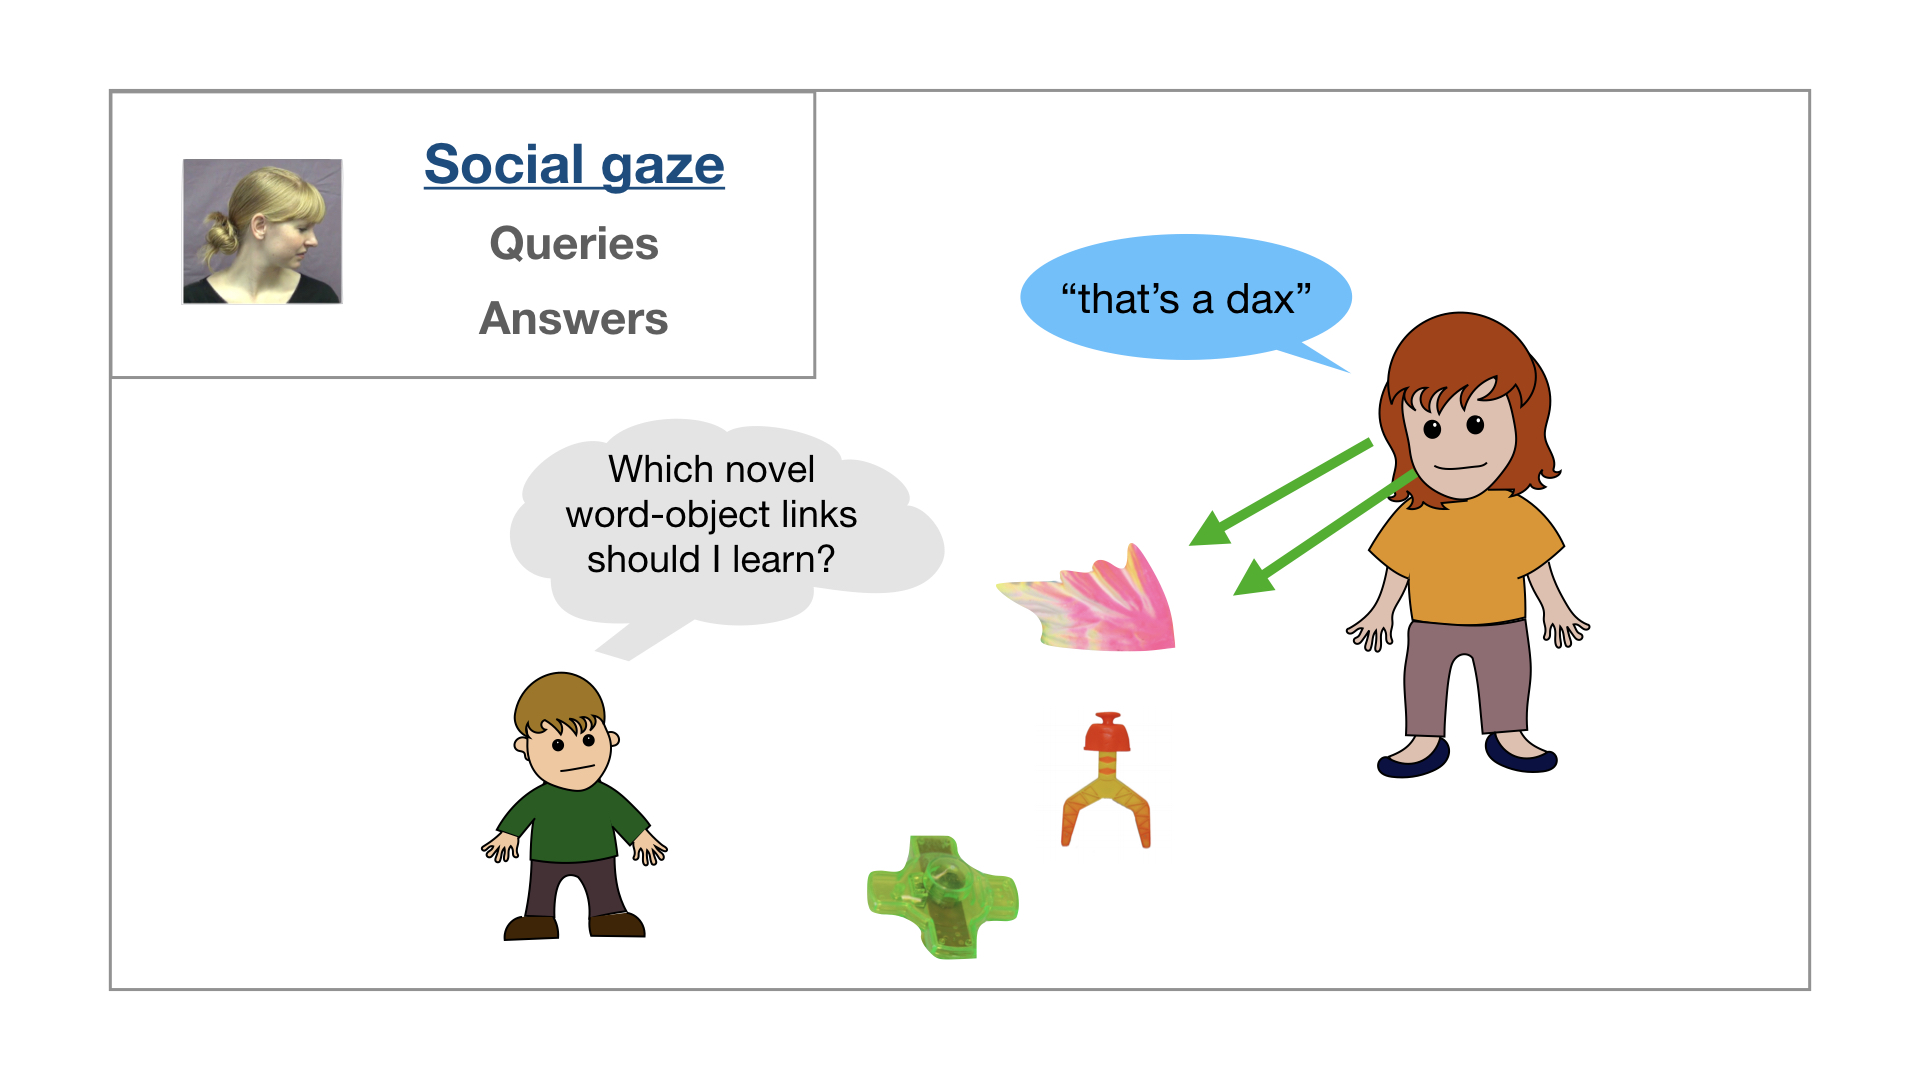
\includegraphics[width=0.9\linewidth]{/Users/ejyoon/Documents/Documents/Research/dissertation/index/chapter_child_rmds/SOC-XSIT/figures/soc_xsit} 

}

\caption[Overview of Chapter 4.]{A schematic showing the components of the active-social learning framework addressed by the case studies in Chapter 4.}\label{fig:schematic-soc-xsit}
\end{figure}
\section{Introduction}\label{introduction-3}

Learning the meaning of a new word should be hard. Consider that even
concrete nouns are often used in complex contexts with multiple possible
referents, which in turn have many conceptually natural properties that
a speaker could talk about. This ambiguity creates the potential for an
(in principle) unlimited amount of referential uncertainty in the
learning task.\footnote{This problem is a simplified version of Quine's
  \textit{indeterminacy of reference} (Quine, 1960): That there are many
  possible meanings for a word (``Gavigai'') that include the referent
  (``Rabbit'') in their extension, e.g., ``white,'' ``rabbit,''
  ``dinner.'' Quine's broader philosophical point was that different
  meanings (``rabbit'' and ``undetached rabbit parts'') could actually
  be extensionally identical and thus impossible to tease apart.}
Remarkably, word learning proceeds despite this uncertainty, with
estimates of adult vocabularies ranging between 50,000 to 100,000
distinct words (P. Bloom, 2002). How do learners infer and retain such a
large variety of word meanings from data with this kind of ambiguity?

Statistical learning theories offer a solution to this problem by
aggregating cross-situational statistics across labeling events to
identify underlying word meanings (Siskind, 1996; C. Yu \& Smith, 2007).
Recent experimental work has shown that both adults and young infants
can use word-object co-occurrence statistics to learn words from
individually ambiguous naming events (Smith \& Yu, 2008; Vouloumanos,
2008). For example, Smith and Yu (2008) taught 12-month-olds three novel
words simply by repeating consistent novel word-object pairings across
10 ambiguous exposure trials. Moreover, computational models suggest
that cross-situational learning can scale up to learn adult-sized
lexicons, even under conditions of considerable referential uncertainty
(K. Smith, Smith, \& Blythe, 2011).

Although all cross-situational learning models agree that the input is
the co-occurrence between words and objects and the output is stable
word-object mappings, they disagree about how closely learners
approximate the input distribution (for review, see Smith, Suanda, \& Yu
2014). One approach has been to model learning as a process of updating
connection strengths between multiple word-object links (McMurray,
Horst, \& Samuelson, 2012), while other approaches have argued that
learners store only a single word-object hypothesis (Trueswell, Medina,
Hafri, \& Gleitman, 2013). In recent experimental and modeling work
Yurovsky and Frank (2015) suggest an integrative explanation: learners
allocate a fixed amount of attention to a single hypothesis and
distribute the rest evenly among the remaining alternatives. As the set
of alternatives grows, the amount of attention allocated to each object
approaches zero.

In addition to the debate about representation, researchers have
disagreed about how to characterize the ambiguity of the input to
cross-situational learning mechanisms. One way to quantify the
uncertainty in a naming event is to show adults video clips of
caregiver-child interactions and measure their accuracy at guessing the
meaning of an intended referent (Human Simulation Paradigm: HSP
{[}Gillette, Gleitman, Gleitman, and Lederer, 1999{]}). Using the HSP,
Medina, Snedeker, Trueswell, and Gleitman (2011) found that
approximately 90\% of learning episodes were ambiguous (\textless{} 33\%
accuracy) and only 7\% were relatively unambiguous (\textgreater{} 50\%
accuracy). In contrast, Yurovsky, Smith, and Yu (2013) found a higher
proportion of clear naming events, with approximately 30\% being
unambiguous (\textgreater{} 90\% accuracy). Consistent with this
finding, Cartmill, Armstrong, Gleitman, Goldin-Meadow, Medina, and
Trueswell (2013) showed that the proportion of unambiguous naming
episodes varies across parent-child dyads, with some parents rarely
providing highly informative contexts and others' doing so relatively
more often.\footnote{The differences in the estimates of referential
  uncertainty in these studies could be driven by the different sampling
  procedures used to select naming events for the HSP. Yurovsky, Smith,
  and Yu (2013) sampled utterances for which the parent labeled a
  co-present object, whereas Medina, Snedeker, Trueswell, et al. (2011)
  randomly sampled any utterances containing concrete nouns. Regardless
  of these differences, the key point here is that variability in
  referential uncertainty across naming events exists and thus could
  alter the representations underlying cross-situational learning.}

Thus, representations in cross-situational word learning can appear
distributional or discrete, and the input to statistical learning
mechanisms can vary along a continuum from low to high ambiguity. These
results raise an interesting question: could learners be sensitive to
the ambiguity of the input and use this information to alter the
representations they store in memory? In the current line of work, we
investigated how the presence of referential cues in the social context
might alter the ambiguity of the input to statistical word learning
mechanisms.

Social-pragmatic theories of language acquisition emphasize the
importance of social cues for word learning (P. Bloom, 2002; E. V.
Clark, 2009; Hollich et al., 2000). Experimental work has shown that
even children as young as 16 months prefer to map novel words to objects
that are the target of a speaker's gaze and not their own (Baldwin,
1993). In an analysis of naturalistic parent-child labeling events, Yu
and Smith (2012) found that young learners tended to retain labels that
were accompanied by clear referential cues, which served to make a
single object dominant in the visual field. And correlational studies
have demonstrated strong links between early intention-reading skills
(e.g., gaze following) and later vocabulary growth (Brooks \& Meltzoff,
2005, 2008; Carpenter, Nagell, Tomasello, Butterworth, \& Moore, 1998).
Moreover, studies outside the domain of language acquisition have shown
that the presence of social cues: (a) produce better spatial learning of
audiovisual events (R. Wu, Gopnik, Richardson, \& Kirkham, 2011), (b)
boost recognition of a cued object (Cleveland, Schug, \& Striano, 2007),
and (c) lead to preferential encoding of an object's featural
information (J. M. Yoon, Johnson, \& Csibra, 2008). Together, the
evidence suggests that social cues could alter the representations
stored during cross-situational word learning by modulating how people
allocate attention to the relevant statistics in the input.

The goal of our current investigation was to ask whether the presence of
a valid social cue -- a speaker's gaze -- could change the
representations underlying cross-situational word learning. We used a
modified version of Yurovsky and Frank (2015)'s paradigm to provide a
direct measure of memory for alternative word-object links during
cross-situational learning. In Experiment 1, we manipulated the presence
of a referential cue at different levels of attention and memory
demands. At all levels of difficulty, learners tracked a strong single
hypothesis but were less likely to track multiple word-object links when
a social cue was present. In Experiment 2, we replicated the findings
from Experiment 1 using a more ecologically valid social cue. In
Experiment 3, we moved to a parametric manipulation of referential
uncertainty by varying the reliability of the speaker's gaze. Learners
were sensitive to graded changes in reliability and retained more
word-object links as uncertainty in the input increased. Finally, in
Experiment 4, we equated the length of the initial naming events with
and without the referential cue. Learners stored less information in the
presence of gaze even when they had visually inspected the objects for
the same amount of time. In sum, our data suggest that cross-situational
word learners are quite flexible, storing representations with different
levels of fidelity depending on the amount of ambiguity present during
learning.

\section{Experiment 1}\label{experiment-1-1}

We set out to test the effect of a referential cue on the
representations underlying cross-situational word learning. We used a
version of Yurovsky and Frank (2015)'s paradigm where we manipulated the
ambiguity of the learning context by including a gaze cue from a
schematic, female interlocutor. Participants saw a series of ambiguous
exposure trials where they heard one novel word that was either paired
with a gaze cue or not and selected the object they thought went with
each word. In subsequent test trials, participants heard the novel word
again, this time paired with a new set of novel objects. One of the
objects in this set was either the participant's initial guess (Same
test trials) or one of the objects was \emph{not} their initial guess
(Switch test trials). Performance on Switch trials provided a direct
measure of whether referential cues influenced the number of alternative
word-object links that learners stored in memory. If learners performed
worse on Switch trials after an exposure trial with gaze, this would
suggest that they stored fewer additional objects from the initial
learning context.

\subsection{Method}\label{method}

\subsubsection{Participants}\label{participants-4}

We posted a set of Human Intelligence Tasks (HITs) to Amazon Mechanical
Turk. Only participants with US IP addresses and a task approval rate
above 95\% were allowed to participate, and each HIT paid 30 cents.
50-100 HITs were posted for each of the 32 between-subjects conditions.
Data were excluded if participants completed the task more than once or
if participants did not respond correctly on familiar object trials (131
HITs). The final sample consisted of 1438 participants.
\begin{figure}[!t]

{\centering 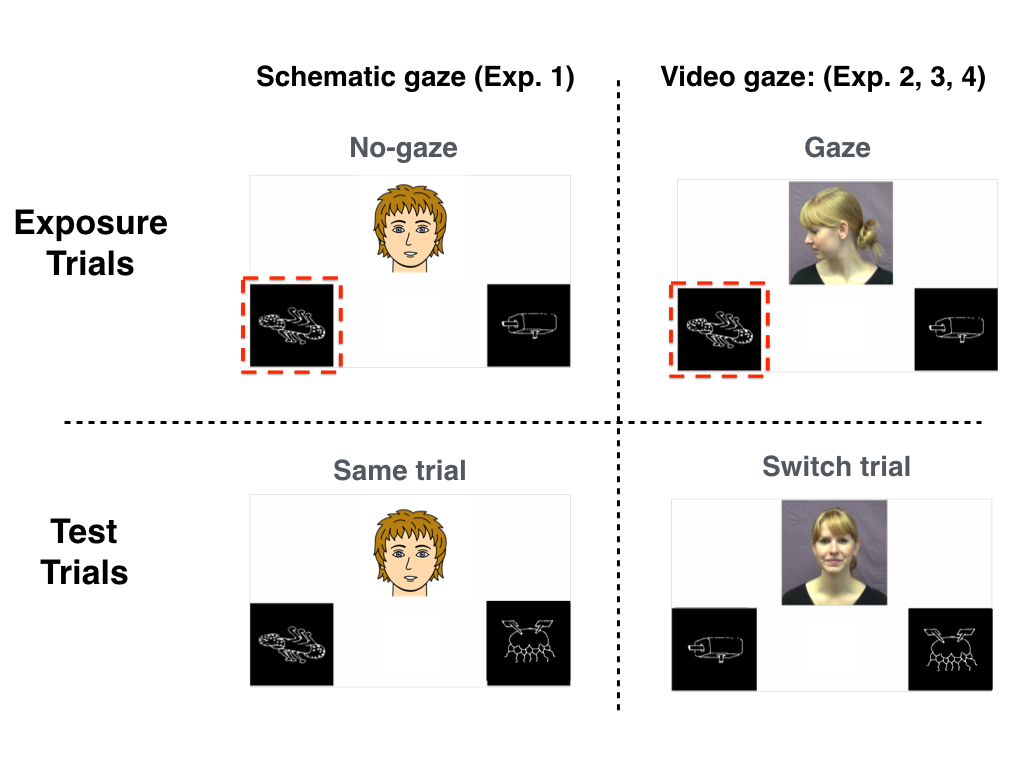
\includegraphics[width=0.9\linewidth]{/Users/ejyoon/Documents/Documents/Research/dissertation/index/chapter_child_rmds/SOC-XSIT/figures/stimuli_new} 

}

\caption[Examples of stimuli for exposure and test trials from Experiments 4.1-4.4.]{Screenshots of exposure and test trials from Experiments 1-4. The top left panel shows an exposure trial in the No-gaze condition using the schematic gaze cue (Experiment 4.1). The top right panel shows an exposure trial in the Gaze condition using the video gaze cue (Experiments 4.2-4.4). Participants saw either Gaze or No-gaze exposure trials depending on condition assignment, and participants saw both types of test trials: Same (bottom left panel) and Switch (bottom right panel). On Same trials, the object that participants chose during exposure appeared with a new novel object. On Switch trials the object that participants did not choose appeared with a new novel object. Participants either saw 2, 4, 6, or 8 referents on the screen depending on condition assignment.}\label{fig:stimuli}
\end{figure}
\subsubsection{Stimuli}\label{stimuli-1}

Figure 1 shows screenshots taken from Experiment 1. Visual stimuli were
black and white pictures of familiar and novel objects taken from
Kanwisher, Woods, Iacoboni, and Mazziotta (1997). Auditory stimuli were
recordings of familiar and novel words by an AT\&T Natural Voices
\texttrademark (voice: Crystal) speech synthesizer. Novel words were 1-3
syllable pseudowords that obeyed all rules of English phonotactics. A
schematic drawing of a human speaker was chosen for ease of manipulating
the direction of gaze, the referential cue of interest in this study.
All experiments can be viewed and downloaded at the project page:
\url{https://kemacdonald.github.io/soc_xsit/}.

\subsubsection{Design and Procedure}\label{design-and-procedure}

Participants saw a total of 16 trials: eight exposure trials and eight
test trials. On each trial, they heard one novel word, saw a set of
novel objects, and were asked to guess which object went with the word.
Before seeing exposure and test trials, participants completed four
practice trials with familiar words and objects. These trials
familiarized participants to the task and allowed us to exclude
participants who were unlikely to perform the task as directed, either
because of inattention or because their computer audio was turned off.

After the practice trials, participants were told that they would now
hear novel words and see novel objects and that their task was to select
the referent that ``goes with each word.'' Over the course of the
experiment, participants heard eight novel words two times, with one
exposure trial and one test trial for each word. Four of the test trials
were \emph{Same} trials in which the object that participants selected
on the exposure trial was shown with a set of new novel objects. The
other four test trials were \emph{Switch} trials in which one of the
objects was chosen at random from the set of objects that the
participant did not select on exposure.

Participants were randomly assigned to one of the 32 between-subjects
conditions (4 Referents X 4 Intervals X 2 Gaze conditions). Participants
either saw 2, 4, 6, or 8 referents on the screen and test trials
occurred at different intervals after exposure trials: either 0, 1, 3,
or 7 trials from the initial exposure to a word. For example, in the
0-interval condition, the test trial for that word would occur
immediately following the exposure trial, but in the 3-interval
condition, participants would see three additional exposure trials for
other novel words before seeing the test trial for the initial word. The
interval conditions modulated the time delay and the number of
intervening trials between learning and test, and the number of
referents conditions modulated the attention demands present during
learning.

Participants were assigned to either the Gaze or No-Gaze condition. In
the Gaze condition, gaze was directed towards one of the objects on
exposure trials; in the No-Gaze condition, gaze was always directed
straight ahead (see Figure 1 for examples). At test, gaze was always
directed straight ahead. To show participants that their response had
been recorded, a red box appeared around the selected object for one
second. This box always appeared around the selected object, even if
participants' selections were incorrect.

\subsection{Results and Discussion}\label{results-and-discussion-3}

\subsubsection{Analysis plan}\label{analysis-plan}

The structure of our analysis plan is parallel across all four
experiments. First, we examined accuracy on exposure trials in the Gaze
condition and then we compared response times on exposure trials across
the Gaze and No-Gaze conditions. These analyses tested whether learners
were (a) sensitive to our experimental manipulation and (b) altered
their allocation of attention in response to the presence of a social
cue. Accuracy on exposure trials was defined as selecting the referent
that was the target of gaze in the Gaze condition. (Note that there was
no ``correct'' behavior for exposure trials in the No-Gaze condition.)
Next, we examined accuracy on test trials to test whether learners'
memory for alternative word-object links changed depending on the
ambiguity of the learning context. Accuracy on test trials (both Same
and Switch) was defined as selecting the referent that was present
during the exposure trial for that word.

The key behavioral prediction of our hypothesis was that the presence of
gaze would result in reduced memory for multiple word-object links,
operationalized as a decrease in accuracy on Switch test trials after
seeing exposure trials with a gaze cue. To quantify participants'
behavior, we used mixed-effects regression models with the maximal
random effects structure justified by our experimental design:
by-subject intercepts and slopes for each trial type (Barr, Levy,
Scheepers, \& Tily, 2013b). We limited all models to include only
two-way interactions because the critical test of our hypothesis was the
interaction between gaze condition and trial type, and we did not have
theoretical predictions for any possible three-way or four-way
interactions.

In the main text, we only report effects that achieved statistical
significance at the \(\alpha\) = .05 threshold. In the Appendix, we
report the full model specification and output for each of the models in
the paper. All models were fit using the lme4 package in R (D. Bates,
Maechler, Bolker, \& Walker, 2013), and all of our data and our
processing/analysis code can be viewed in the version control repository
for this paper at \url{https://github.com/kemacdonald/soc_xsit}.
\begin{figure}[!t]

{\centering 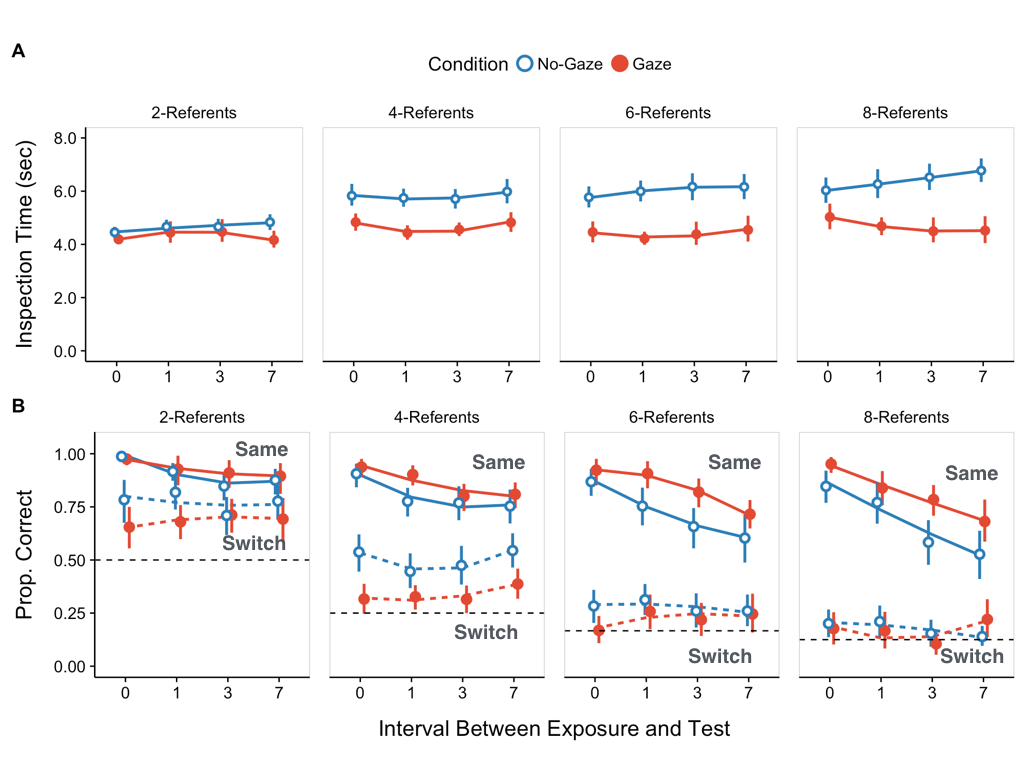
\includegraphics[width=0.9\linewidth]{/Users/ejyoon/Documents/Documents/Research/dissertation/index/chapter_child_rmds/SOC-XSIT/figures/expt1_new} 

}

\caption[Experiment 4.1 results.]{Experiment 4.1 results. The top row shows average inspection times on exposure trials for all experimental conditions as a function of the number of trials that occurred between exposure and test. Each panel represents a different number of referents, and line color represents the Gaze and No-Gaze conditions. The bottom row shows accuracy on test trials for all conditions as a function of the number of intervening trials. The horizontal dashed lines represent chance performance for each number of referents, and the type of line (solid vs. dashed) represents the different test trial types (Same vs. Switch). Error bars indicate 95\% confidence intervals computed by non-parametric bootstrap.}\label{fig:expt1-plot}
\end{figure}
\subsubsection{Exposure trials}\label{exposure-trials}

To ensure that our referential cue manipulation was effective, we
compared participants' accuracies on exposure trials in the Gaze
condition to a model of random behavior defined as a Binomial
distribution with a probability of success \(\frac{1}{Num Referents}\).
Correct performance was defined as selecting the object that was the
target of the speaker's gaze. Following Yurovsky and Frank (2015), we
fit logistic regressions for each gaze, referent, and interval
combination specified as
\texttt{Gaze Target $\sim$ 1 + offset(logit(1/Referents))}. The offset
encoded the chance probability of success given the number of referents,
and the coefficient for the intercept term shows on a log-odds scale how
much more likely participants were to select the gaze target than would
be expected if participants were selecting randomly. In all conditions,
participants used gaze to select referents on exposure trials more often
than expected by chance (smallest \(\beta\) = 1.4, z = 9.38, \(p\)
\textless{} .001). However, the mean proportion of gaze following varied
across conditions (overall \(M\) = 0.84, range: 0.77--0.93).

We were also interested in differences in participants' response times
across the experimental conditions. Since these trials were self-paced,
participants could choose how much time to spend inspecting the
referents on the screen, thus providing an index of participants'
attention. To quantify the effects of gaze, interval, and number of
referents, we fit a linear mixed-effects model that predicted
participants' inspection times as follows:
\texttt{Log(Inspection time) $\sim$ (Gaze * Log(Interval) + Log(Referents))$^2$ + (1 | subject)}.
We found a significant main effect of the number of referents (\(\beta\)
= 0.34, p \textless{} .001) with longer inspection times as the number
of referents increased, a significant interaction between gaze condition
and the number of referents (\(\beta\) = -0.27, p \textless{} .001) with
longer inspection times in the No-Gaze condition, especially as the
number of referents increased, and a significant interaction between
gaze condition and interval (\(\beta\) = -0.08, \(p\) = 0.004) with
longer inspection times in the No-Gaze condition, especially as the
number of intervening trials increased (see the top row of Figure 2).
Shorter inspection times on exposure trials with gaze provide evidence
that the presence of a referential cue focused participants' attention
on a single referent and away from alternative word-object links.

\subsubsection{Test trials}\label{test-trials}

Next, we explored participants' accuracy in identifying the referent for
each word in all conditions for both kinds of test trials (see the
bottom row of Figure 2). We first compared the distribution of correct
responses made by each participant to the distribution expected if
participants were selecting randomly defined as a Binomial distribution
with a probability of success \(\frac{1}{Num Referents}\). Correct
performance was defined as selecting the object that was present on the
exposure trial for that word. We fit the same logistic regressions as we
did for exposure trials:
\texttt{Correct $\sim$ 1 + offset(logit(1/Referents))}. In 31 out of the
32 conditions for both Same and Switch trials, participants chose the
correct object more often than would be expected by chance (smallest
\(\beta\) = 0.36, \(z\) = 2.44, \(p\) = 0.01). On Switch trials in the
8-referent, 3-interval condition, participants' responses were not
significantly different from chance (\(\beta\) = 0.06, z = 0.33, \(p\) =
0.74). Participants' success on Switch trials replicates the findings
from Yurovsky and Frank (2015) and provides direct evidence that
learners encoded more than a single hypothesis in ambiguous word
learning situations even under high attentional and memory demands and
in the presence of a referential cue.
\begin{table}[tb]
\centering
\begin{tabular}{lrrrrl}
 Predictor & Estimate & Std. Error & $z$ value & $p$ value &  \\ 
  \hline
Intercept & 3.01 & 0.29 & 10.35 & $<$ .001 & *** \\ 
  Switch Trial & -1.36 & 0.24 & -5.63 & $<$ .001 & *** \\ 
  Gaze Condition & 0.12 & 0.26 & 0.47 & 0.64 &  \\ 
  Log(Interval) & -0.45 & 0.11 & -4.08 & $<$ .001 & *** \\ 
  Log(Referents) & 0.23 & 0.11 & 2.02 & 0.04 & * \\ 
  Switch Trial*Gaze Condition & -1.09 & 0.12 & -9.07 & $<$ .001 & *** \\ 
  Switch Trial*Log(Interval) & 0.52 & 0.05 & 9.50 & $<$ .001 & *** \\ 
  Switch Trial*Log(Referent) & -0.59 & 0.09 & -6.49 & $<$ .001 & *** \\ 
  Gaze Condition*Log(Interval) & 0.06 & 0.06 & 1.00 & 0.32 &  \\ 
  Gaze Condition*Log(Referent) & 0.20 & 0.09 & 2.15 & 0.03 & * \\ 
  Log(Interval)*Log(Referent) & -0.04 & 0.04 & -1.02 & 0.31 &  \\ 
   \hline
\end{tabular}
\caption{Predictor estimates with standard errors and significance information for a logistic mixed-effects model predicting word learning in Experiment 4.1.} 
\label{tab:exp1_reg}
\end{table}
To quantify the effects of gaze, interval, and number of referents on
the probability of a correct response, we fit the following
mixed-effects logistic regression model to a filtered dataset where we
removed participants who did not reliably select the object that was the
target of gaze on exposure trials:\footnote{We did not predict that
  there would be a subset of participants who would not follow the gaze
  cue, thus this filtering criterion was developed posthoc. However, we
  think that the filter is theoretically motivated because we would only
  expect to see an effect of gaze if participants actually used the gaze
  cue. The filter removed 94 participants (6\% of the sample). The key
  inferences from the data do not depend on this filtering criterion.}
\texttt{Correct $\sim$ (Trial Type + Gaze + Log(Interval) + Log(Referents))$^2$ + offset(logit($^1/_{Referents}$)) + (TrialType | subject)}.
We coded interval and number of referents as continuous predictors and
transformed these variables to the log scale.\footnote{If we allowed for
  three-way interactions in the model, the key interaction between gaze
  condition and trial type remained significant (\(\beta\) = -1.3, \(p\)
  = 0.006).}

Table 1 shows the output of the logistic regression. We found
significant main effects of the number of referents (\(\beta = 0.23\),
\(p\) \textless{} .001) and interval (\(\beta = -0.45\), \(p\)
\textless{} .001), such that as each of these factors increased,
accuracy on test trials decreased. We also found a significant main
effect of trial type (\(\beta = -1.36\), \(p\) \textless{} .001), with
worse performance on Switch trials. There were significant interactions
between trial type and interval (\(\beta = 0.52\), \(p\) \textless{}
.001), trial type and referents (\(\beta = -0.59\), \(p\) \textless{}
.001), and gaze condition and referents (\(\beta = 0.2\), \(p\)
\textless{} .05). These interactions can be interpreted as meaning: (a)
the interval between exposure and test affected Same trials more than
Switch trials, (b) the number of referents affected Switch trials more
than Same trials, and (c) participants performed slightly better at the
higher number of referents in the Gaze condition. The interactions
between gaze condition and referents and between referents and interval
were not significant. Importantly, we found the predicted interaction
between trial type and gaze condition (\(\beta = -1.09\), \(p\)
\textless{} .001), with participants in the Gaze condition performing
worse on Switch trials. This interaction provides direct evidence that
the presence of a referential cue reduces participants' memory for
alternative word-object links.

We were also interested in how the length of inspection times on
exposure trials would affect participants' accuracy at test. So we fit
an additional model where participants' inspection times were included
as a predictor. We found a significant interaction between inspection
time and gaze condition (\(\beta = -0.17\), \(p\) = 0.01) such that
longer inspection times provided a larger boost to accuracy in the
No-Gaze condition. Importantly, the key test of our hypothesis, the
interaction between gaze condition and trial type, remained significant
in this alternative version of the model (\(\beta\) = -1.02, \(p\) = p
\textless{} .001).

Taken together, the inspection time and accuracy analyses provide
evidence that the presence of a referential cue modulated learners'
attention during learning, and in turn made them less likely to track
multiple word-object links. We saw some evidence for a boost to
performance on Same trials in the Gaze condition at the higher number of
referent and interval conditions, but reduced tracking of alternatives
did not always result in better memory for learners' candidate
hypothesis. This finding suggests that the limitations on Same trials
may be different than those regulating the distribution of attention on
Switch trials.

There was relatively large variation in performance across conditions in
the group-level accuracy scores and in participants' tendency to
\emph{use} the referential cue on exposure trials. Moreover, we found a
subset of participants who did not reliably use the gaze cue at all. It
is possible that the effect of gaze was reduced because the referential
cue that we used -- a static schematic drawing of a speaker -- was
relatively weak compared to the cues present in real-world learning
environments. Thus we do not yet know how learners' memory for
alternatives during cross-situational learning would change in the
presence of a stronger and more ecologically valid referential cue. We
designed Experiment 2 to address this question.

\section{Experiment 2}\label{experiment-2-1}

In Experiment 2, we set out to replicate the findings from Experiment 1
using a more ecologically valid stimulus set. We replaced the static,
schematic drawing with a video of an actress. While these stimuli were
still far from actual learning contexts, they included a real person who
provided both a gaze cue and a head turn towards the target object. To
reduce the across-conditions variability that we found in Experiment 1,
we introduced a within-subjects design where each participant saw both
Gaze and No-Gaze exposure trials in a blocked design. We selected a
subset of the conditions from Experiment 1 and tested only the
4-referent display with 0 and 3 intervening trials as between-subjects
manipulations. Our goals were to replicate the reduction in learners'
tracking of alternative word-object links in the presence of a
referential cue and to test whether increasing the ecological validity
of the cue would result in a boost to the strength of learners' recall
of their candidate hypothesis.

\subsection{Method}\label{method-1}

\subsubsection{Participants}\label{participants-5}

Participant recruitment and inclusion/exclusion criteria were identical
to those of Experiment 1. 100 HITs were posted for each condition (1
Referent X 2 Intervals X 2 Gaze conditions) for a total of 400 paid HITs
(33 HITs excluded).

\subsubsection{Stimuli}\label{stimuli-2}

Audio and picture stimuli were identical to Experiment 1. The
referential cue in the Gaze condition was a video (see Figure 1). On
each exposure trial, the actress looked out at the participant with a
neutral expression, smiled, and then turned to look at one of the four
images on the screen. She maintained her gaze for 3 seconds before
returning to the center. On test trials, she looked straight ahead for
the duration of the trial.

\subsubsection{Design and Procedure}\label{design-and-procedure-1}

Procedures were identical to those of Experiment 1. The major design
change was a within-subjects manipulation of the gaze cue where each
participant saw exposure trials with and without gaze. The experiment
consisted of 32 trials split into 2 blocks of 16 trials. Each block
consisted of 8 exposure trials and 8 test trials (4 Same trials and 4
Switch trials) and contained only Gaze or No-gaze exposure trials. The
order of block was counterbalanced across participants.

\subsection{Results and Discussion}\label{results-and-discussion-4}

We followed the same analysis plan as in Experiment 1. We first analyzed
inspection times and accuracy on exposure trials and then analyzed
accuracy on test trials.

\subsubsection{Exposure trials}\label{exposure-trials-1}

Similar to Experiment 1, participants' responses on exposure trials
differed from those expected by chance (smallest \(\beta\) = 3.39, z =
31.99, \(p\) \textless{} .001), suggesting that gaze was effective in
directing participants' attention. Participants in Experiment 2 were
more consistent in their use of gaze with the video stimuli compared to
the schematic stimuli used in Experiment 1 (\(M_{Exp1}\) = 0.8,
\(M_{Exp2}\) = 0.91), suggesting that using a real person increased
participants' willingness to follow the gaze cue.

We replicated the findings from Experiment 1. Inspection times were
shorter when gaze was present (\(\beta\) = -1.1, \(p\) \textless{} .001)
and in the 3-interval condition (\(\beta\) = -0.48, \(p\) \textless{}
.001). The interaction between gaze and interval was not significant,
meaning that gaze had the same effect on participants' inspection times
at both intervals (see Panel A of Figure 3).
\begin{figure}[!t]

{\centering 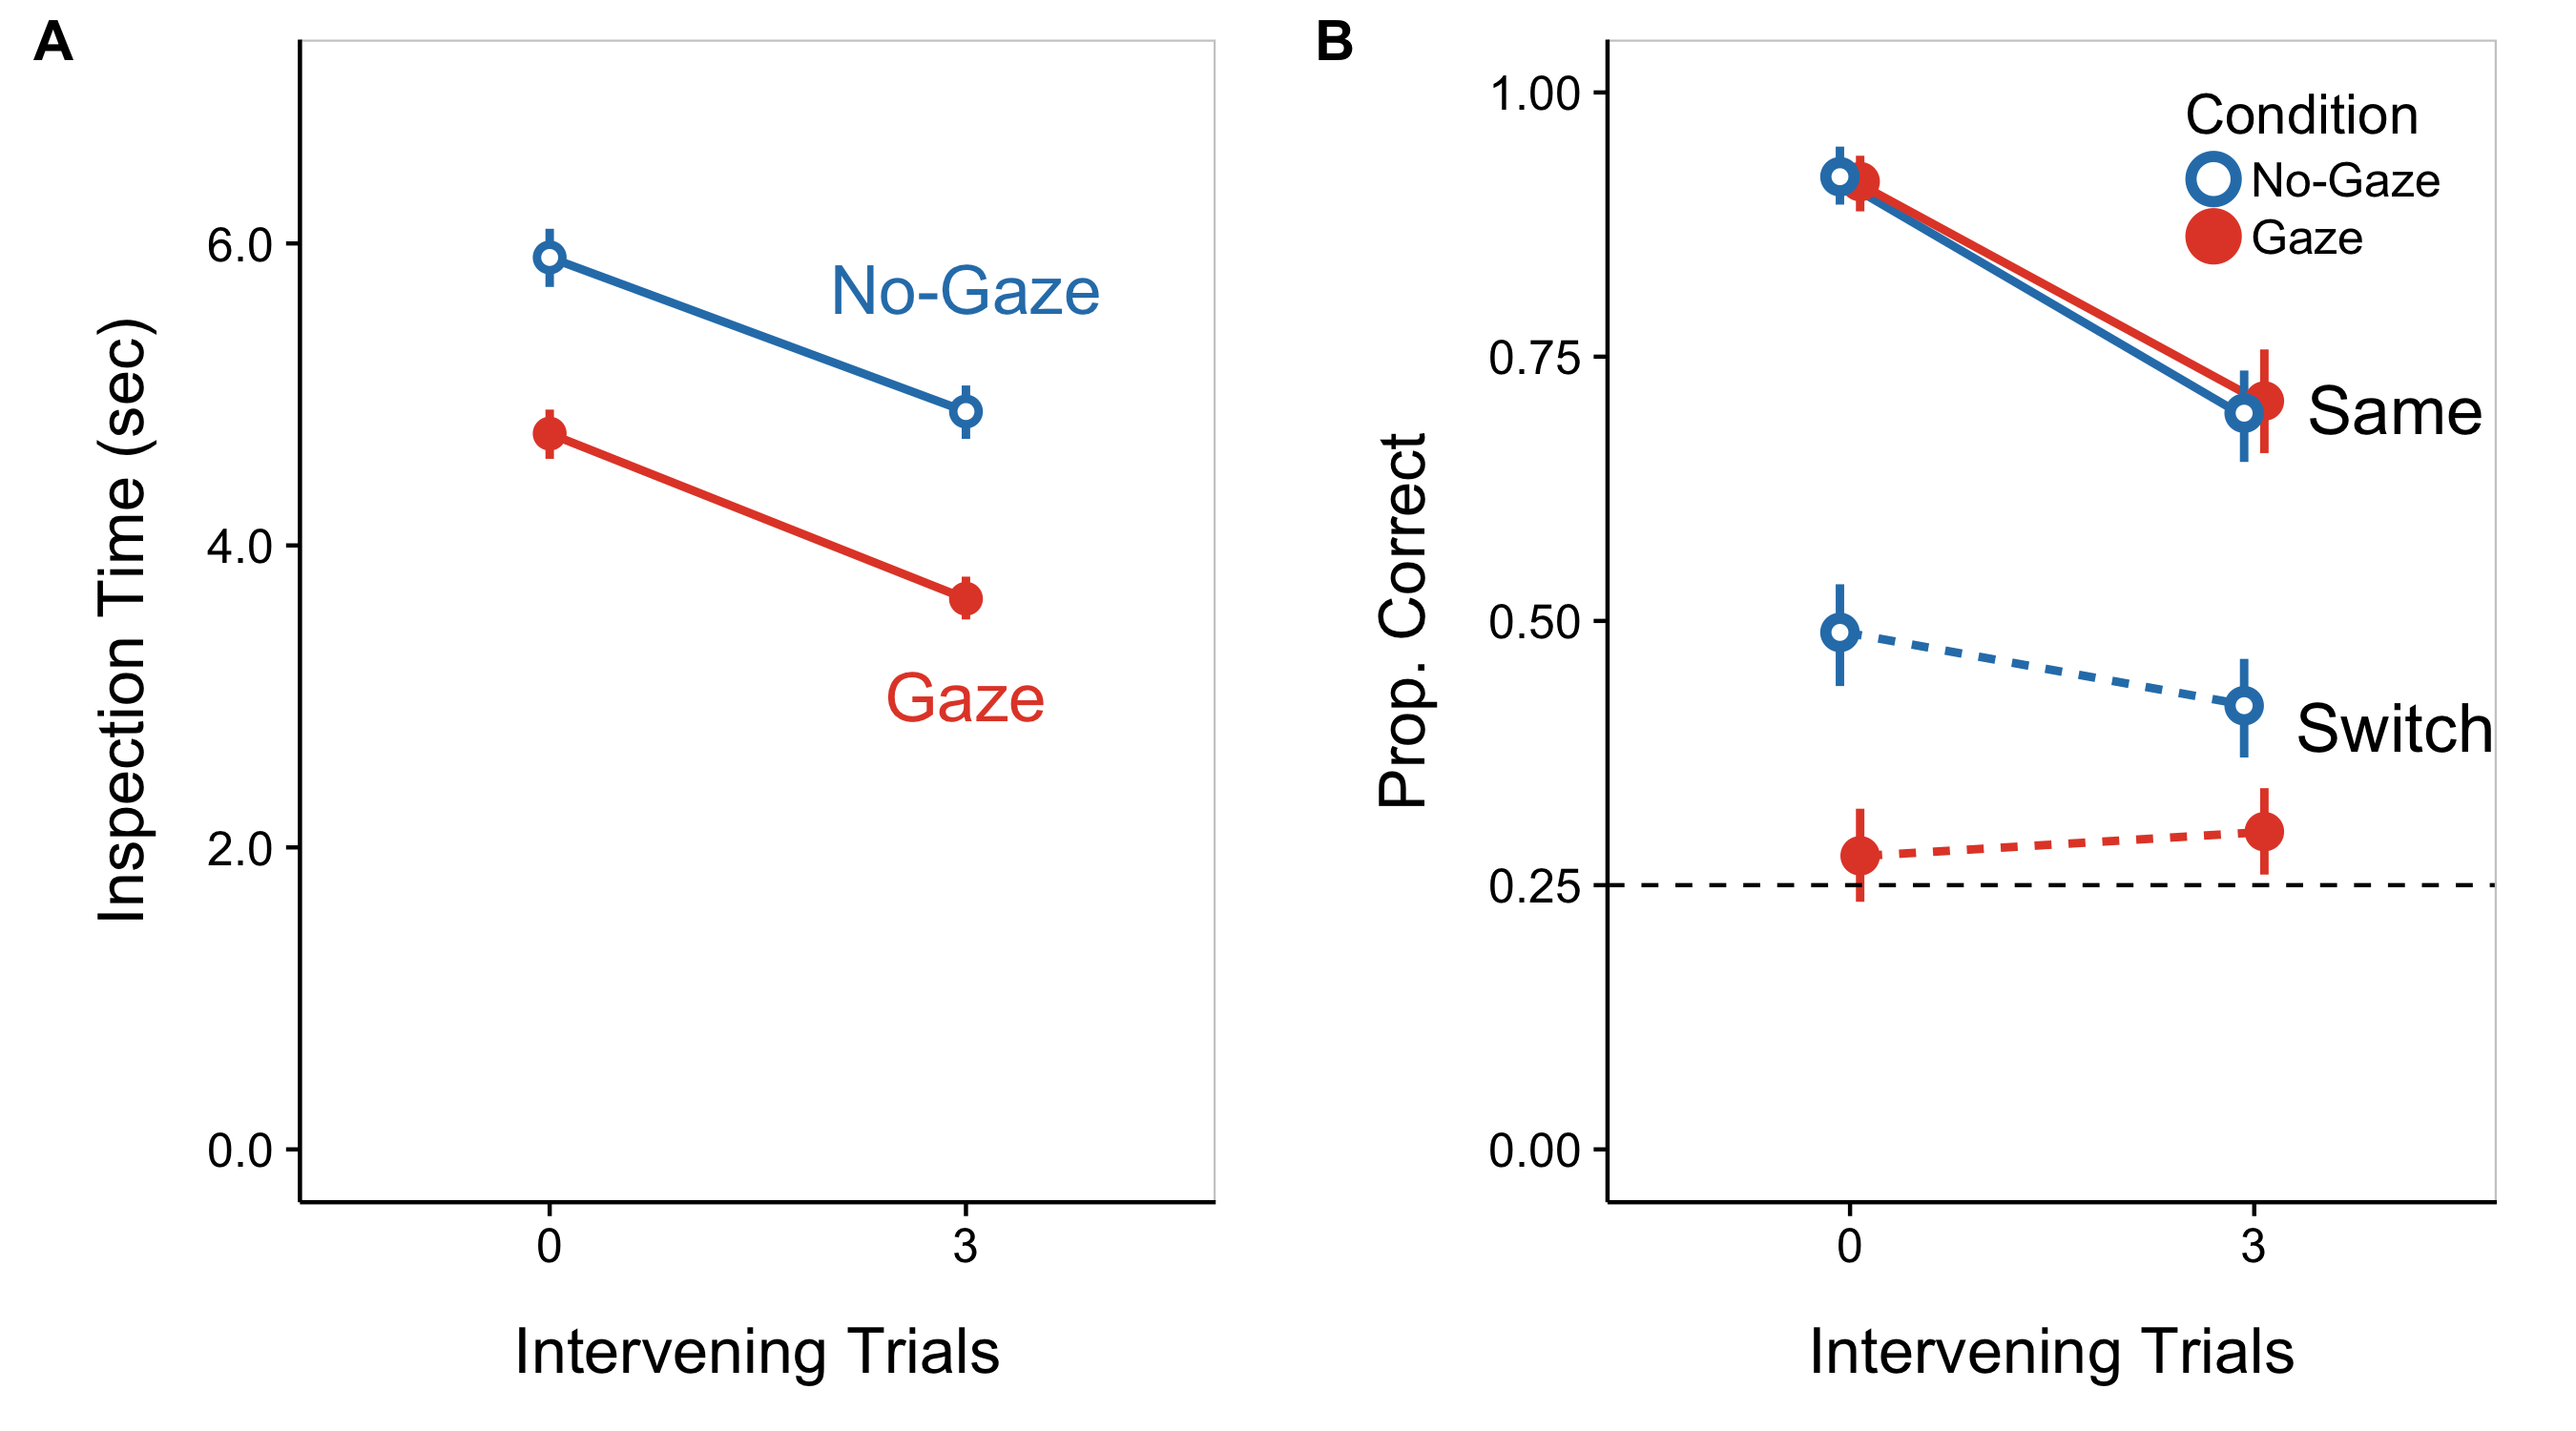
\includegraphics[width=0.9\linewidth]{/Users/ejyoon/Documents/Documents/Research/dissertation/index/chapter_child_rmds/SOC-XSIT/figures/expt2_new} 

}

\caption[Experiment 4.2 results]{Experiment 2 results. Panel A shows inspection times on exposure trials with and without gaze. Panel B shows accuracy on Same and Switch test trials. All plotting conventions are the same as in Figure 2. Error bars indicate 95\% confidence intervals computed by non-parametric bootstrap.}\label{fig:expt2-plot}
\end{figure}
\subsubsection{Test trials}\label{test-trials-1}
\begin{table}[tb]
\centering
\begin{tabular}{lrrrrl}
 Predictor & Estimate & Std. Error & $z$ value & $p$ value &  \\ 
  \hline
Intercept & 4.04 & 0.18 & 21.97 & $<$ .001 & *** \\ 
  Switch Trial & -2.99 & 0.19 & -16.11 & $<$ .001 & *** \\ 
  Gaze Condition & -0.10 & 0.16 & -0.63 & 0.53 &  \\ 
  Log(Interval) & -0.93 & 0.10 & -9.23 & $<$ .001 & *** \\ 
  Switch Trial*Gaze Condition & -0.71 & 0.16 & -4.49 & $<$ .001 & *** \\ 
  Switch Trial*Log(Interval) & 0.79 & 0.10 & 8.03 & $<$ .001 & *** \\ 
  Gaze Condition*Log(Interval) & 0.15 & 0.08 & 2.05 & 0.04 & * \\ 
   \hline
\end{tabular}
\caption{Predictor estimates with standard errors and significance information for a logistic mixed-effects model predicting word learning in Experiment 4.2.} 
\label{tab:exp2_reg}
\end{table}
Across all conditions for both trial types, participants selected the
correct referent at rates greater than chance (smallest \(\beta\) =
0.58, z = 9.32, \(p\) \textless{} .001). We replicated the critical
finding from Experiment 1: after seeing exposure trials with gaze,
participants performed worse on Switch trials, meaning they stored fewer
word-object links (\(\beta = -0.71\), \(p\) \textless{}
.001).\footnote{As in Experiment 1, we fit this model to a filtered dataset removing participants who did not reliably use the gaze cue.}
Participants were also less accurate as the interval between exposure
and test increased (\(\beta\) = -0.93, \(p\) \textless{} .001) and on
the Switch trials overall (\(\beta = -2.99\), \(p\) \textless{} .001).

In addition, there was a significant interaction between trial type and
interval (\(\beta = 0.79\), \(p\) \textless{} .001), with worse
performance on Switch trials in the 3-interval condition. The
interaction between gaze condition and interval was also significant
(\(\beta = 0.15\), \(p\) = 0.041), such that participants in the gaze
condition were less affected by the increase in interval. Similar to
Experiment 1, we did not see evidence of a boost to performance on Same
trials in the gaze condition.

Next, we added inspection times on exposure trials to the model. Similar
to Experiment 1, the key interaction between gaze and trial type
remained significant in this version of the model (\(\beta\) = -0.54,
\(p\) \textless{} .001). We also found an interaction between inspection
time and trial type (\(\beta\) = 0.21, \(p\) = 0.05), with longer
inspection times providing a larger boost to performance on Switch
trials (i.e., stronger memory for alternative word-object links). This
result differs slightly from Experiment 1 where we found an interaction
between trial type and inspection time, with longer inspection times
providing a larger boost to accuracy in the No-Gaze condition. Despite
this subtle difference, we speculate that inspection times likely played
a similar role in both experiments, with longer inspection times leading
to better performance on Switch trials since these trials depended on
encoding multiple word-object links. It is also possible that the
interaction between gaze condition and inspection time that we found in
Experiment 1 was influenced by the different number of referents and
interval conditions.

The results of Experiment 2 provide converging evidence for our primary
hypothesis that the presence of a referential cue reliably focuses
learners' attention away from alternative word-object links and shifts
them towards single hypothesis tracking. Moving to the video stimulus
led to higher rates of selecting the target of gaze on exposure trials,
but did not result in a boost to performance on Same trials. This
finding suggests that the level of attention and memory demand present
in the learning context might modulate the effect of gaze on the
fidelity of learners' single hypothesis.

Thus far we have shown that people store different amounts of
information in response to a categorical manipulation of referential
uncertainty. In both Experiments 1 and 2, the learning context was
either entirely ambiguous (No-Gaze) or entirely unambiguous (Gaze). But
not all real-world learning contexts fall at the extremes of this
continuum. Could learners be sensitive to more subtle changes in the
quality of the input? In our next experiment, we tested a prediction of
our account: whether learners would store more word-object links in
response to graded changes in referential uncertainty during learning.

\section{Experiment 3}\label{experiment-3-2}

In Experiment 3, we explored whether learners would allocate attention
and memory flexibly in response to \emph{graded} changes in the
referential uncertainty that was present during learning. To test this
hypothesis, we moved beyond a categorical manipulation of the
presence/absence of gaze, and we parametrically varied the reliability
of the referential cue. We manipulated cue reliability by adding a block
of familiarization trials where we varied the proportion of Same and
Switch trials. If participants saw more Switch trials, this provided
direct evidence that the speaker's gaze was a less reliable cue to
reference because the gaze target on exposure trials would not appear at
test. This design was inspired by a growing body of experimental work
showing that even young children are sensitive to the prior reliability
of speakers and will use this information to decide whom to learn novel
words from (e.g., Koenig, Clement, \& Harris, 2004).

\subsection{Method}\label{method-2}

\subsubsection{Participants}\label{participants-6}

Participant recruitment and inclusion/exclusion criteria were identical
to those of Experiment 1 and 2 (27 HITs excluded). 100 HITs were posted
for each reliability level (0\%, 25\%, 50\%, 75\%, and 100\%) for total
of 500 paid HITs.

\subsubsection{Design and Procedure}\label{design-and-procedure-2}

Procedures were identical to those of Experiments 1 and 2. We modified
the design of our cross-situational learning paradigm to include a block
of 16 familiarization trials (8 exposure trials and 8 test trials) at
the beginning of the experiment. These trials served to establish the
reliability of the speaker's gaze. To establish reliability, we varied
the proportion of Same/Switch trials that occurred during the
familiarization block. Recall that on Switch trials the gaze target did
not show up at test, which provided evidence that the speaker's gaze was
not a reliable cue to reference. Reliability was a between-subjects
manipulation such that participants either saw 8, 6, 4, 2, or 0 Switch
trials during familiarization, which created the 0\%, 25\%, 50\%, 75\%,
and 100\% reliability conditions. After the familiarization block,
participants completed another block of 16 trials (8 exposure trials and
8 test trials). Since we were no longer testing the effect of the
presence or absence of a referential cue, all exposure trials throughout
the experiment included a gaze cue. Finally, at the end of the task, we
asked participants to assess the reliability of the speaker on a
continuous scale from ``completely unreliable'' to ``completely
reliable.''

\subsection{Results and Discussion}\label{results-and-discussion-5}

\subsubsection{Exposure trials}\label{exposure-trials-2}

Participants reliably chose the referent that was the target of gaze at
rates greater than chance (smallest \(\beta\) = 2.62, z = 31.99, \(p\)
\textless{} .001). We fit a mixed effects logistic regression model
predicting the probability of selecting the gaze target as follows:
\texttt{Correct-Exposure $\sim$ Reliability Condition * Subjective Reliability + (1 | subject)}.
We found an effect of reliability condition (\(\beta\) = 3.28, \(p\) =
0.03) such that when the gaze cue was more reliable, participants were
more likely to use it (\(M_{0\%}\) = 0.83, \(M_{25\%}\) = 0.82,
\(M_{50\%}\) = 0.87, \(M_{75\%}\) = 0.9, \(M_{100\%}\) = 0.94). We also
found an effect of subjective reliability (\(\beta\) = 7.26, \(p\)
\textless{} .001) such that when participants thought the gaze cue was
reliable, they were more likely to use it. This analysis provides
evidence that participants were sensitive to the reliability
manipulation both in how often they used the gaze cue and in how they
rated the reliability of the speaker at the end of the task.

\subsubsection{Test trials}\label{test-trials-2}
\begin{figure}[!t]

{\centering 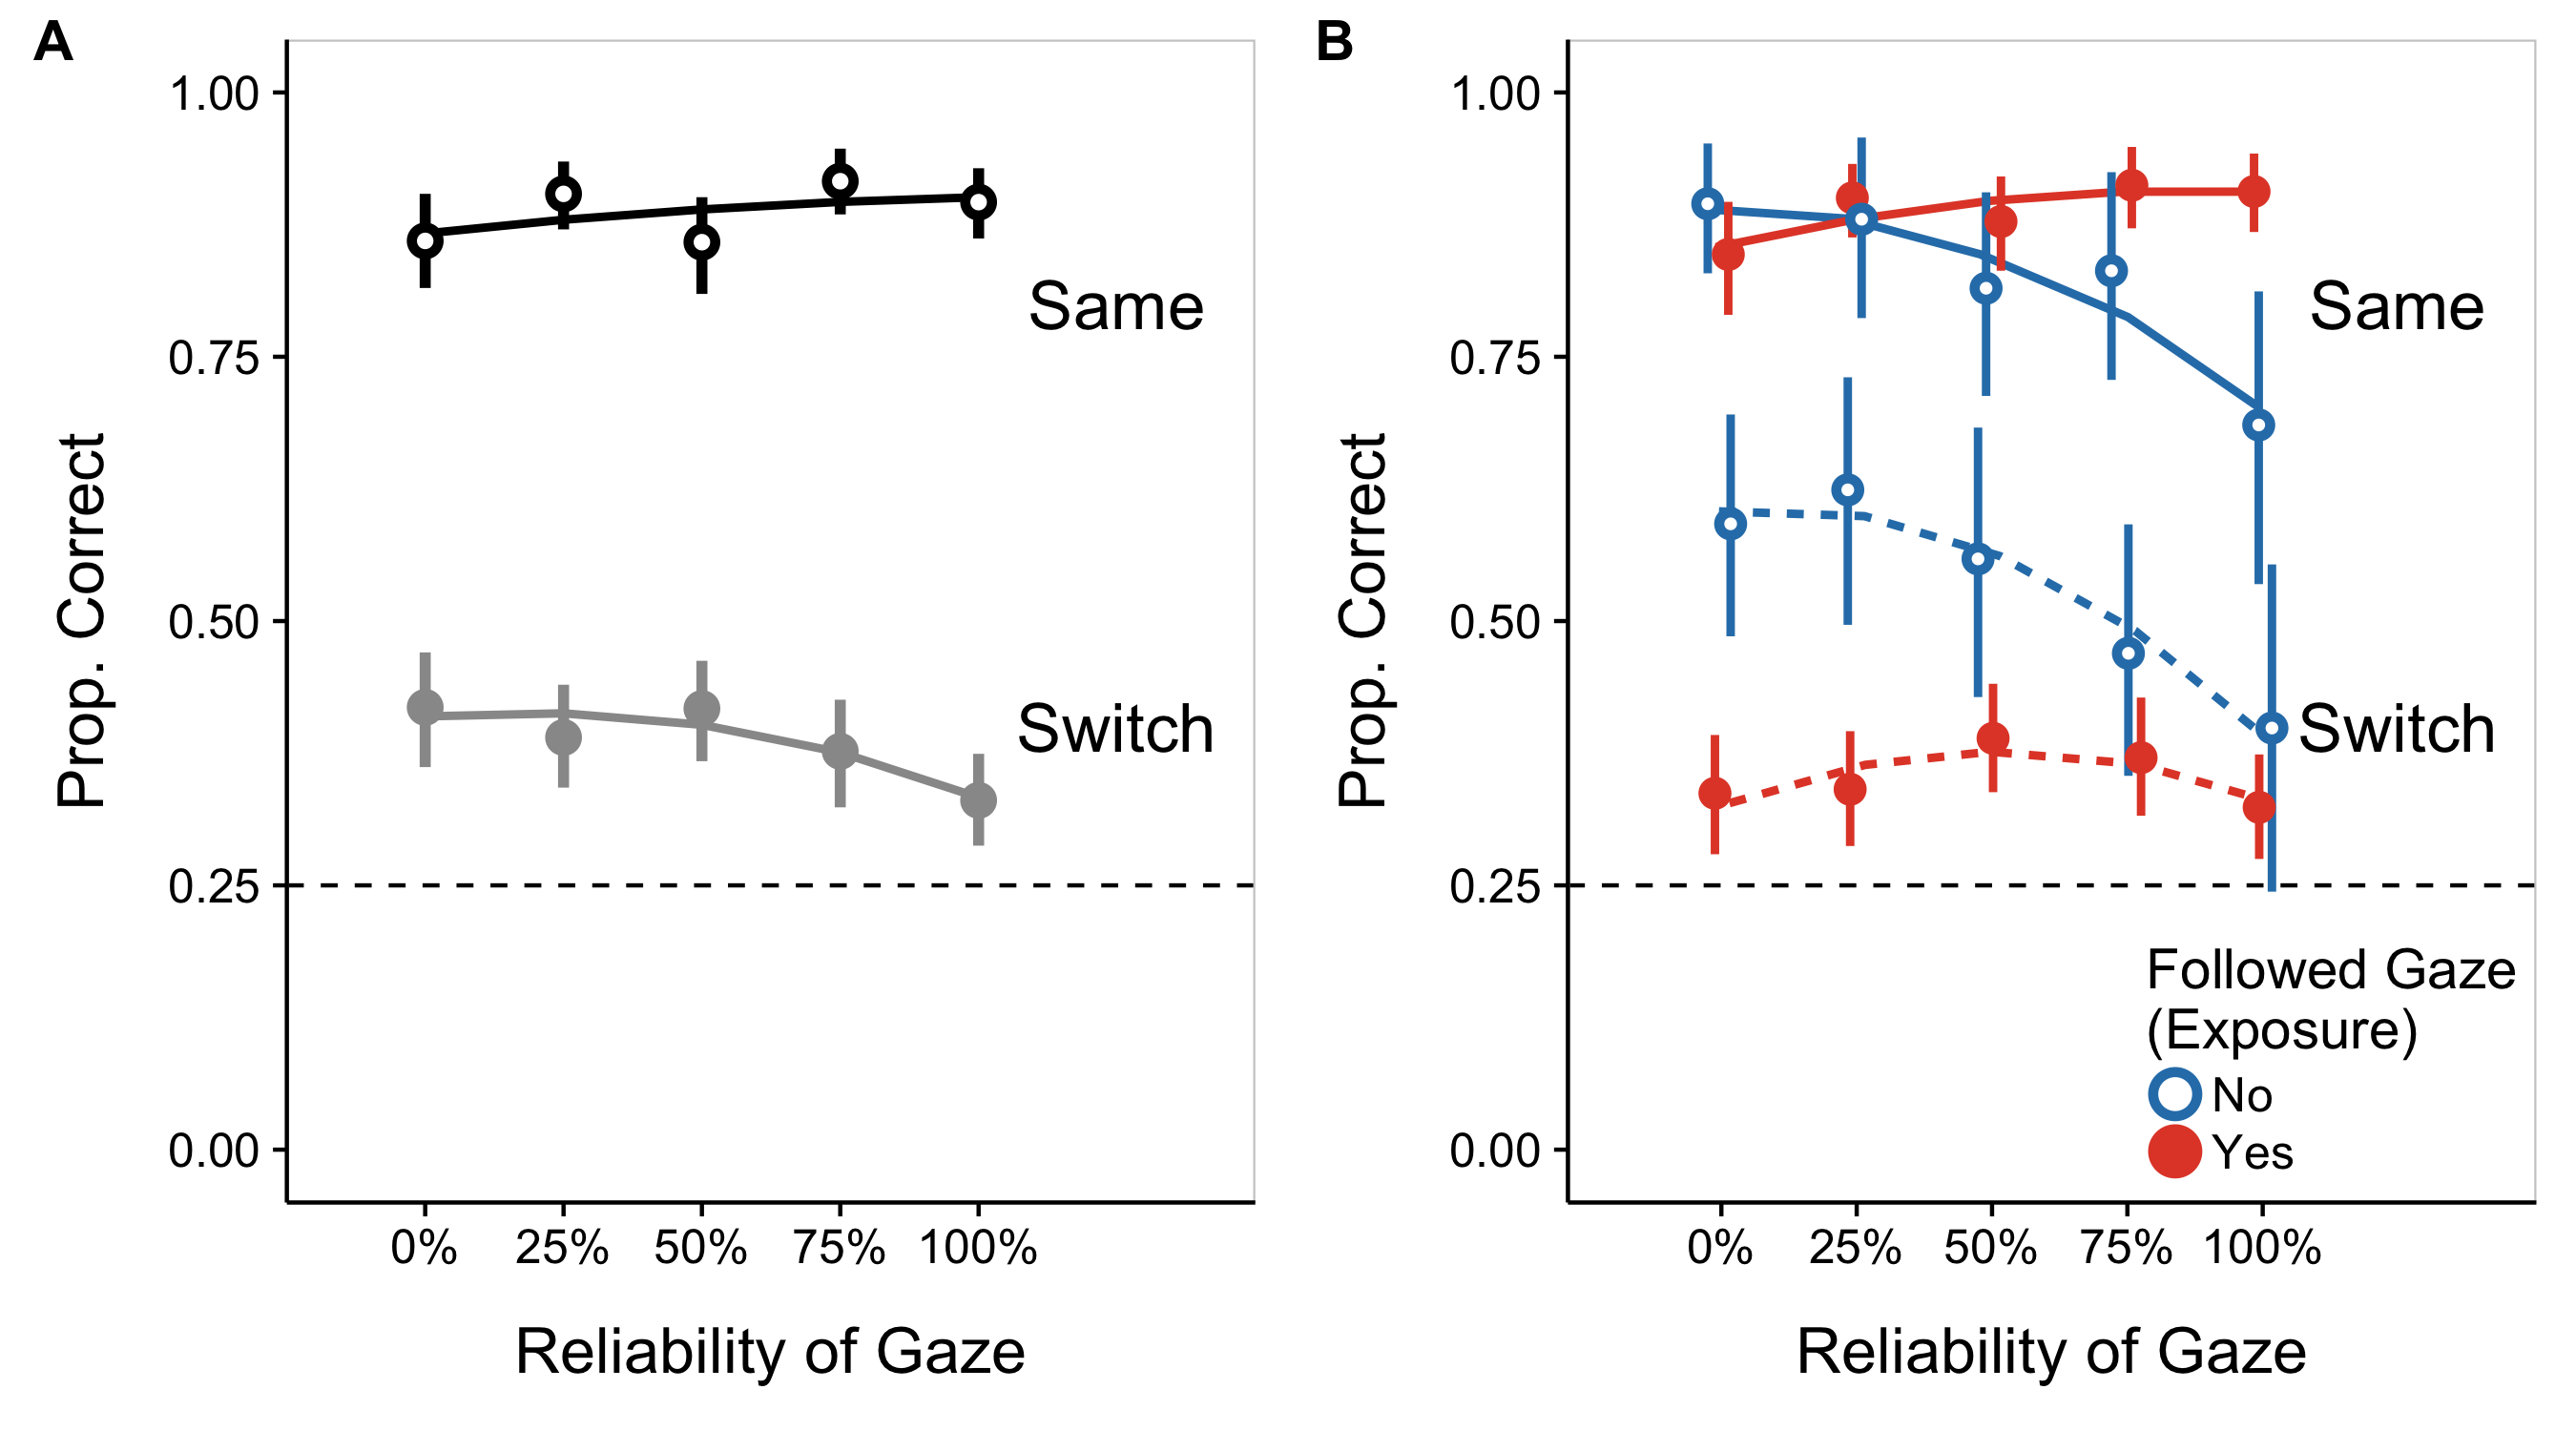
\includegraphics[width=0.9\linewidth]{/Users/ejyoon/Documents/Documents/Research/dissertation/index/chapter_child_rmds/SOC-XSIT/figures/expt3_main_plot} 

}

\caption[Primary analyses of test trial performance in Experiment 4.3]{Primary analyses of test trial performance in Experiment 3. Panel A shows performance as a function of reliability condition. Panel B shows performance as a function of reliability condition and whether participants chose to follow gaze on exposure trials. The horizontal dashed lines represent chance performance, and error bars indicate 95\% confidence intervals computed by non-parametric bootstrap.}\label{fig:e3-plot}
\end{figure}
Next, we tested whether the reliability manipulation altered the
strength of participants' memory for alternative word-object links in
the second block of test trials that followed the initial
familiarization phase. Across all conditions, participants selected the
correct referent at rates greater than chance (smallest \(\beta\) =
0.42, z = 3.69, \(p\) \textless{} .001). Our primary prediction was an
interaction between reliability and test trial type, with higher levels
of reliability leading to worse performance on Switch trials (i.e., less
memory allocated to alternative word-object links). To explore this
prediction, we performed four complementary analyses: our primary
analysis, which tested the effect of the reliability manipulation, and
three secondary analyses, which explored the effects of participants'
(a) use of the gaze cue, (b) subjective reliability assessments, and (c)
inspection time on exposure trials.
\begin{figure}[!t]

{\centering 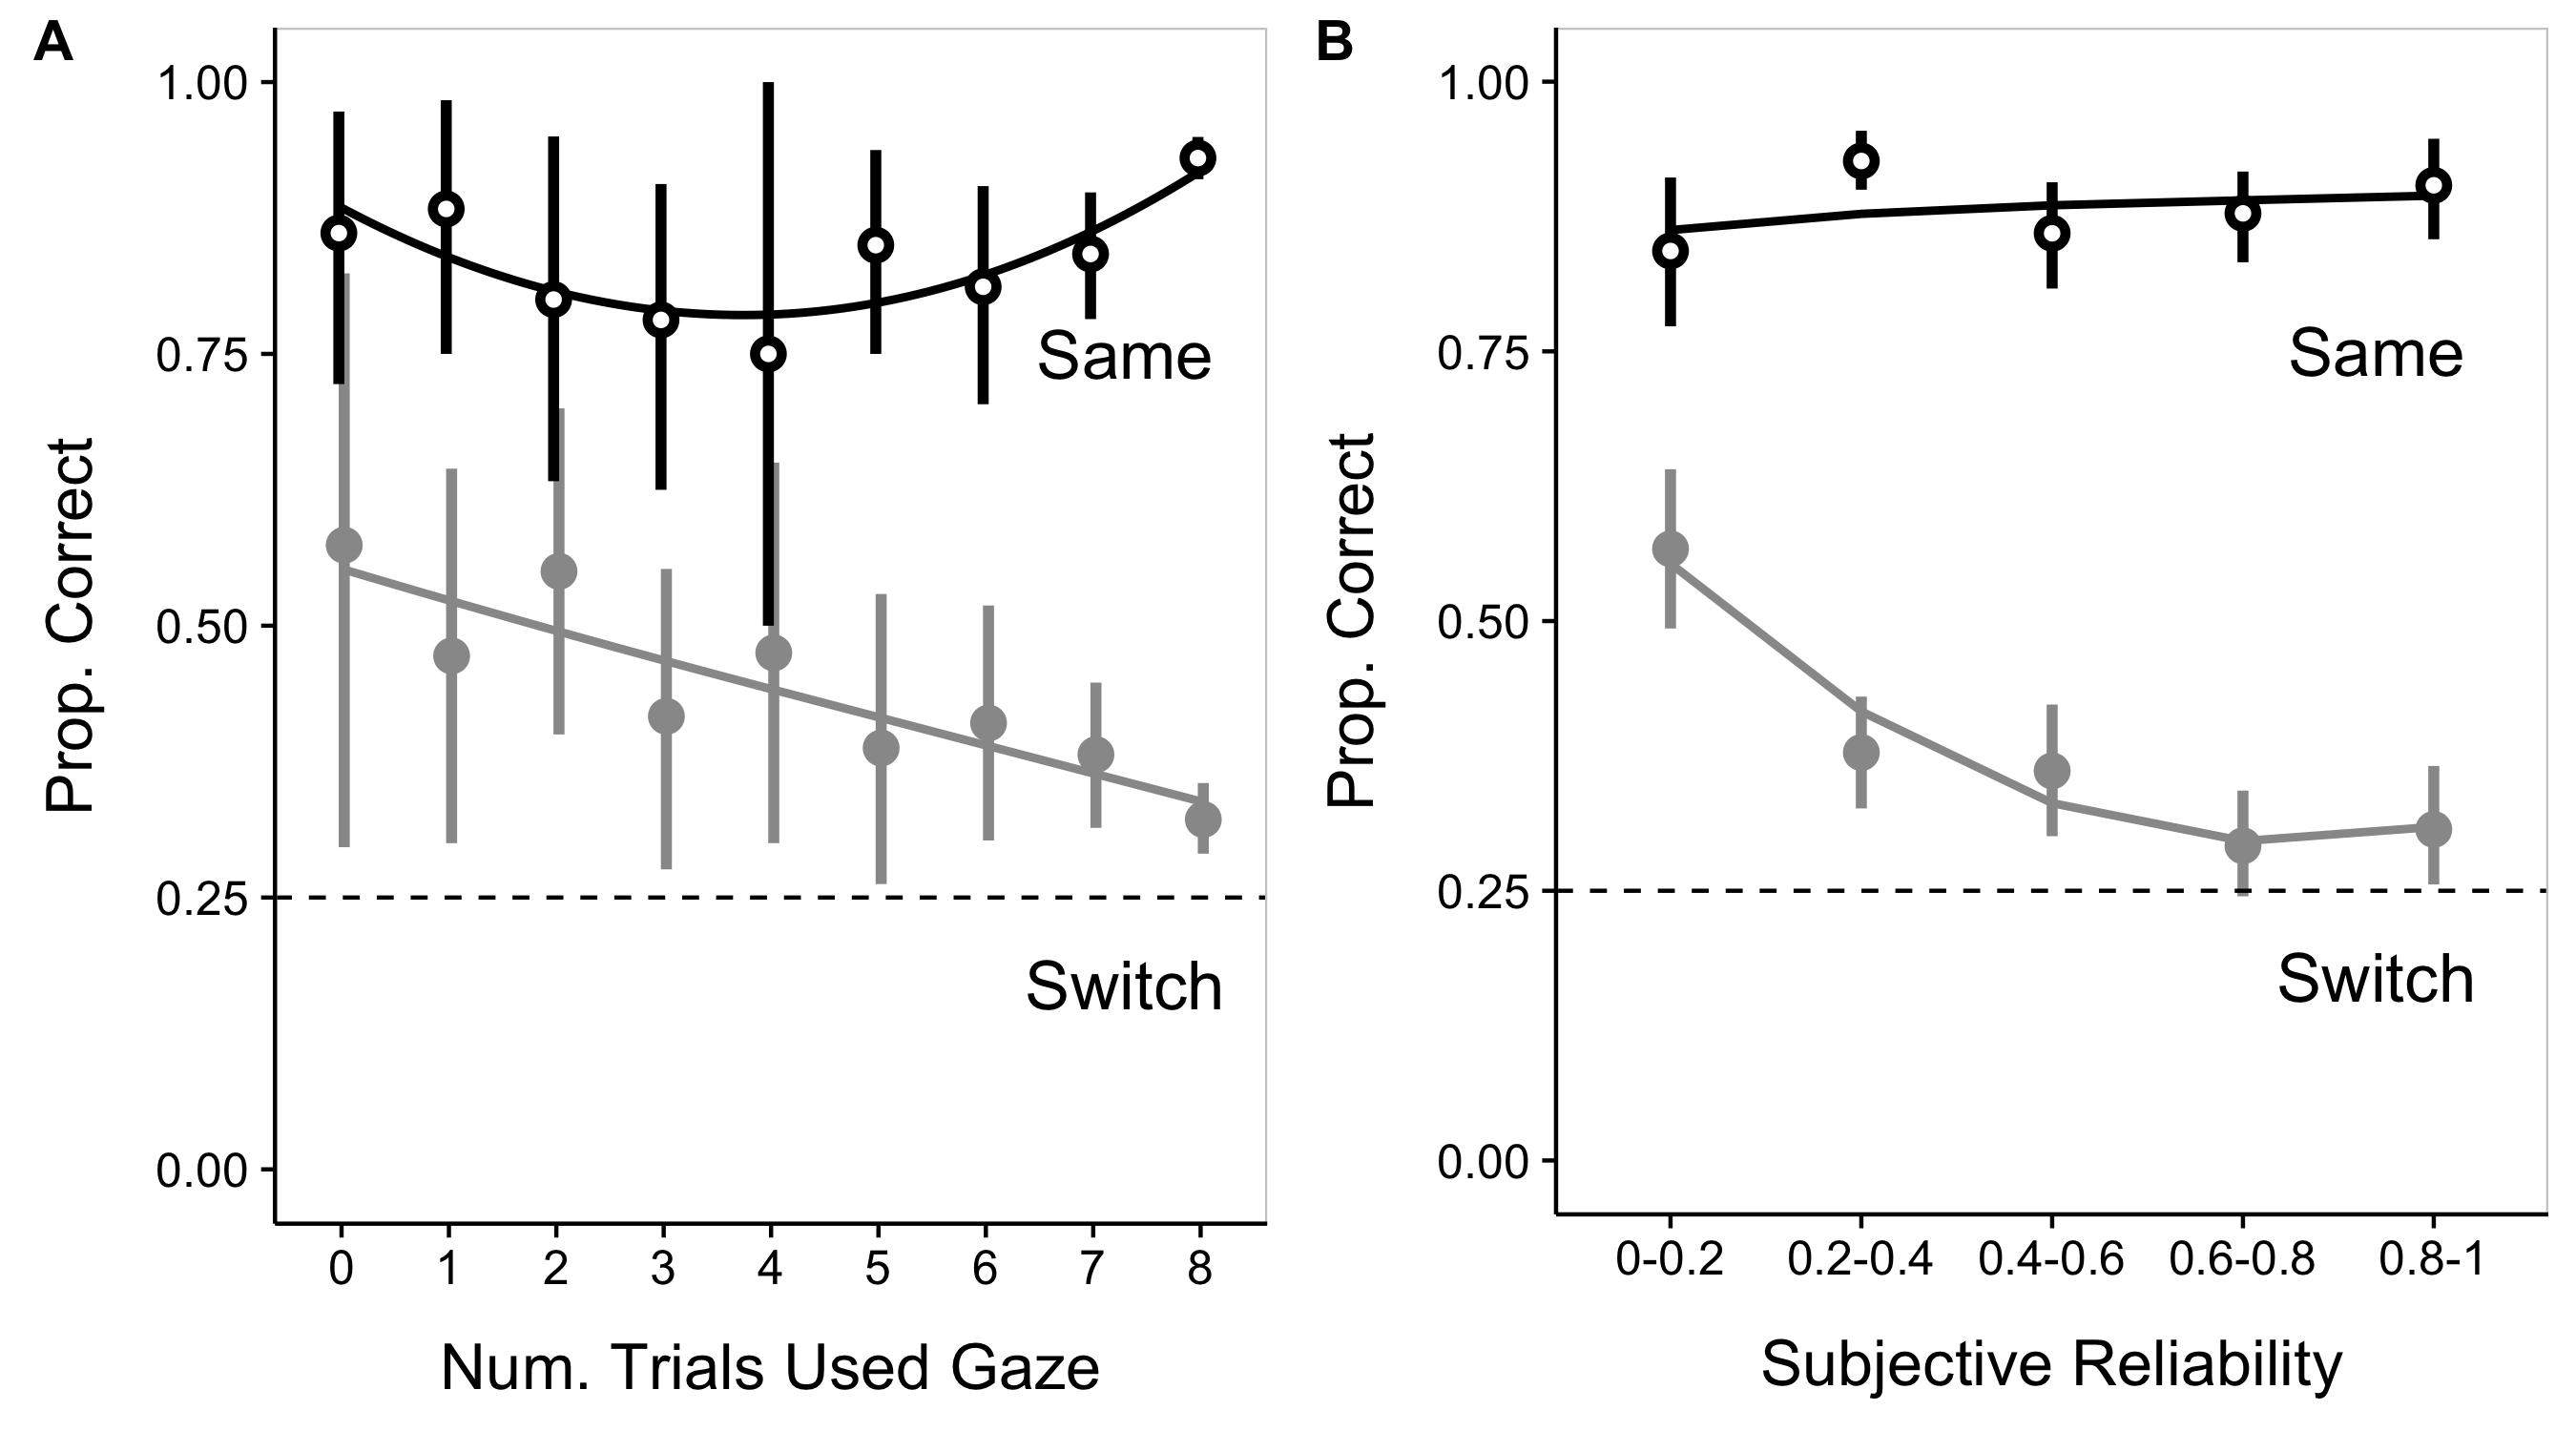
\includegraphics[width=0.9\linewidth]{/Users/ejyoon/Documents/Documents/Research/dissertation/index/chapter_child_rmds/SOC-XSIT/figures/expt3_sub_plot} 

}

\caption[Secondary analyses of test trial performance in Experiment 4.3]{Secondary analyses of test trial performance in Experiment 3. Panel A shows accuracy as a function of the number of exposure trials on which participants chose to use the gaze cue. Panel B shows accuracy as a function of participants' subjective reliability judgments. The horizontal dashed lines represent chance performance, and error bars indicate 95\% confidence intervals computed by non-parametric bootstrap.}\label{fig:expt3-sub-plots}
\end{figure}
\subsubsection{Reliability condition
analysis}\label{reliability-condition-analysis}

To test the effect of reliability, we fit a model predicting accuracy at
test using reliability condition and test trial type as predictors. We
found a significant main effect of trial type (\(\beta = -3.95\), \(p\)
\textless{} .001), with lower accuracy on Switch trials. We also found
the key interaction between reliability condition and trial type
(\(\beta\) = -0.76, \(p\) = 0.044), such that when gaze was more
reliable, participants performed worse on Switch trials (see Panel A of
Figure 4). This interaction suggests that people store more word-object
links as the learning context becomes more ambiguous. However, the
interaction between reliability and trial type was not particularly
strong, and -- similar to Experiment 1 -- performance varied across
conditions (see the 50\% reliable condition in Panel A of Figure 4). So
to provide additional support for our hypothesis, we conducted three
follow-up analyses.

\subsubsection{Gaze use analyses}\label{gaze-use-analyses}

We would only expect to see a strong interaction between reliability and
trial type if learners chose to use the gaze cue during exposure trials.
To test this hypothesis, we fit two additional models that included two
different measures of participants' use of the gaze cue. First, we added
the number of exposure trials on which participants chose to use the
gaze cue as a predictor in our model. We found a significant interaction
between use of the gaze cue on exposure trials and trial type
(\(\beta = -1.43\), \(p\) \textless{} .001) with worse performance on
Switch test trials when participants used gaze on exposure trials (see
Panel B of Figure 4). We also found an interaction between gaze use and
reliability (\(\beta = 0.97\), \(p\) = 0.004) such that when gaze was
more reliable, participants were more likely to use it. The \(\beta\)
value for the interaction between trial type and reliability changed
from -0.76 to -0.62, (\(p\) = 0.086). This reduction suggests that
participants' tendency to use the gaze cue is a stronger predictor of
learners' memory for alternative word-object links compared to our
reliability manipulation.\footnote{We are grateful to an anonymous
  reviewer for suggesting this analysis, but we would like to note that
  it is exploratory.}

We also hypothesized that the reliability manipulation might change how
often individual participants chose to use the gaze cue throughout the
task. To explore this possibility, we fit a model with the same
specifications, but we included a predictor that we created by binning
participants based on the number of exposure trials on which they chose
to follow gaze (i.e., a gaze following score). We found a significant
interaction between how often participants chose to follow gaze on
exposure trials and trial type (\(\beta = -0.26\), \(p\) \textless{}
.001), such that participants who were more likely to use the gaze cue
performed worse on Switch trials, but not Same trials (see Panel A of
Figure 5).\footnote{We found this interaction while performing
  exploratory data analyses on a previous version of this study with an
  independent sample (N = 250, \(\beta = -0.24\), \(p\) \textless{}
  .001). The results reported here are from a follow-up study where
  testing this interaction was a planned analysis.} Taken together, the
two analyses of participants' use of the gaze cue provide converging
evidence that when the speaker's gaze was reliable participants were
more likely to use the cue, and when they followed gaze, they tended to
store less information from the initial naming event.

\subsubsection{Subjective reliability
analysis}\label{subjective-reliability-analysis}

The strong interaction between use of the gaze cue and memory for
alternative word-object links suggests that participants' subjective
experience of reliability in the experiment mattered. Thus, we fit the
same model but substituted subjective reliability for the frequency of
gaze use as a predictor of test trial performance. We found a
significant interaction between trial type and participants' subjective
reliability assessments (\(\beta = -1.63\), \(p\) = 0.01): when
participants thought the speaker was more reliable, they performed worse
on Switch trials, but not Same trials (see Panel B of Figure 5).

\subsubsection{Inspection time analyses}\label{inspection-time-analyses}

Finally, we analyzed the effect of inspection times on exposure trials,
fitting a model using inspection time, trial type, and reliability
condition to predict accuracy at test. We found a main effect of
inspection time (\(\beta\) = 0.31, \(p\) = 0.001), with longer
inspection times leading to better performance for both Same and Switch
trials. The interaction between inspection time and reliability
condition was not significant. The key interaction between reliability
condition and trial type remained significant in this version of the
model (\(\beta\) = -0.58, \(p\) = 0.048).

Next, we explored the factors that influenced inspection time on
exposure trials by fitting a model to predict inspection times as a
function of reliability condition and participants' use of the gaze cue.
We found a main effect of participants' use of the gaze cue (-0.32,
\(p\) \textless{} .001) with shorter inspection times when participants
followed gaze. The main effect of reliability condition and the
interaction between reliability and use of gaze were not significant.
These analyses provide evidence that inspection times were similar
across the different reliability conditions and that use of the gaze cue
was the primary factor affecting how long participants explored the
objects during learning.

Together, these four analyses show that when the speaker's gaze was more
reliable, participants were more likely to: (a) use the gaze cue, (b)
rate the speaker as more reliable, and (c) store fewer word-object
links, showing behavior more consistent with single hypothesis tracking.
These findings support and extend the results of Experiments 1 and 2 in
several important ways. First, similar to Experiment 2, participants'
performance on Same trials was relatively unaffected by changes in
performance on Switch trials. The selective effect of gaze on Switch
trials provides converging evidence that the limitations on Same trials
may be different than those regulating the distribution of attention on
Switch trials. Second, learners' use of a referential cue was a stronger
predictor of reduced memory for alternative word-object links compared
to our reliability manipulation. Although we found a significant effect
of reliability on participants' use of the gaze cue, participants'
tendency to use the cue remained high. Consider that even in the 0\%
reliability condition the mean proportion of gaze following was still
0.82. It is reasonable that participants would continue to use the gaze
cue in our experiment since it was the only cue available and
participants did not have a strong reason to think that the speaker
would be deceptive.

The critical contribution of Experiment 3 is to show that learners
respond to a graded manipulation of referential uncertainty, with the
amount of information stored from the initial exposure tracking with the
reliability of the cue. This graded accuracy performance shows that
learners stored alternative word-object links with different levels of
fidelity depending on the amount of referential uncertainty present
during learning.

Across Experiments 1-3, learners tended to store fewer word-object links
in unambiguous learning contexts when a clear referential cue was
present. However, in all three experiments, participants' responses on
exposure trials controlled the length of the trial, meaning that when
participants used the gaze cue, they also spent less time visually
inspecting the objects. Thus, we do not know whether there is an
independent effect of referential cues on the representations underlying
cross-situational learning, or if the effects found in Experiments 1-3
are entirely mediated by a reduction in inspection time. In Experiment
4, we addressed this possibility by removing participants' control over
the length of exposure trials, which made the inspection times
equivalent across the Gaze and No-Gaze conditions.

\section{Experiment 4}\label{experiment-4}

In Experiment 4, we asked whether a reduction in visual inspection time
in the gaze condition could completely explain the effect of social cues
on learners' reduced memory for alternative word-object links. To answer
this question, we modified our paradigm and made the length of exposure
trials equivalent across the Gaze and No-Gaze conditions. In this
version of the task, participants were shown the objects for a fixed
amount of time regardless of whether gaze was present. We also included
two different exposure trial lengths in order to test whether gaze would
have a differential effect at shorter vs.~longer inspection times. If
the presence of gaze reduces learners' memory for multiple word-object
links, then this provides evidence that referential cues affected the
underlying representations over and above a reduction in inspection
time.

\subsection{Method}\label{method-3}

\subsubsection{Participants}\label{participants-7}

Participant recruitment and inclusion/exclusion criteria were identical
to those of Experiments 1, 2, and 3. 100 HITs were posted for each
condition (1 Referent X 2 Intervals X 2 Inspection Time conditions) for
a total of 400 paid HITs (37 HITs excluded).

\subsubsection{Stimuli}\label{stimuli-3}

Audio, picture, and video stimuli were identical to Experiments 2 and 3.
Since inspection times were fixed across conditions, we wanted to ensure
that participants were aware of the time remaining on each exposure
trial. So we included a circular countdown timer located above the
center video. The timer remained on the screen during test trials but
did not count down since participants could take as much time as they
wanted to respond on test trials.

\subsubsection{Design and Procedure}\label{design-and-procedure-3}

Procedures were identical to those of Experiment 1-3. The design was
identical to that of Experiment 2 and consisted of 32 trials split into
2 blocks of 16 trials. Each block consisted of 8 exposure trials and 8
test trials (4 Same trials and 4 Switch trials) and contained only Gaze
or No-Gaze exposure trials. The order of block was counterbalanced
across participants.

The major design change was to make the length of exposure trials
equivalent across the Gaze and No-Gaze conditions. We randomly assigned
participants to one of two inspection time conditions: Short or Long.
Initially, the length of the inspection times was based on participants'
self-paced inspection times in the Gaze and No-Gaze conditions in
Experiment 2 (Short = 3 seconds; Long = 6 seconds). However, after pilot
testing, we added three seconds to each condition to ensure that
participants had enough time to respond before the experiment advanced
(Short = 6 seconds; Long = 9 seconds). If participants did not respond
in the allotted time, an error message appeared informing participants
that time had run out and encouraged them to respond within the time
window on subsequent trials.

\subsection{Results and Discussion}\label{results-and-discussion-6}
\begin{figure}[!t]

{\centering 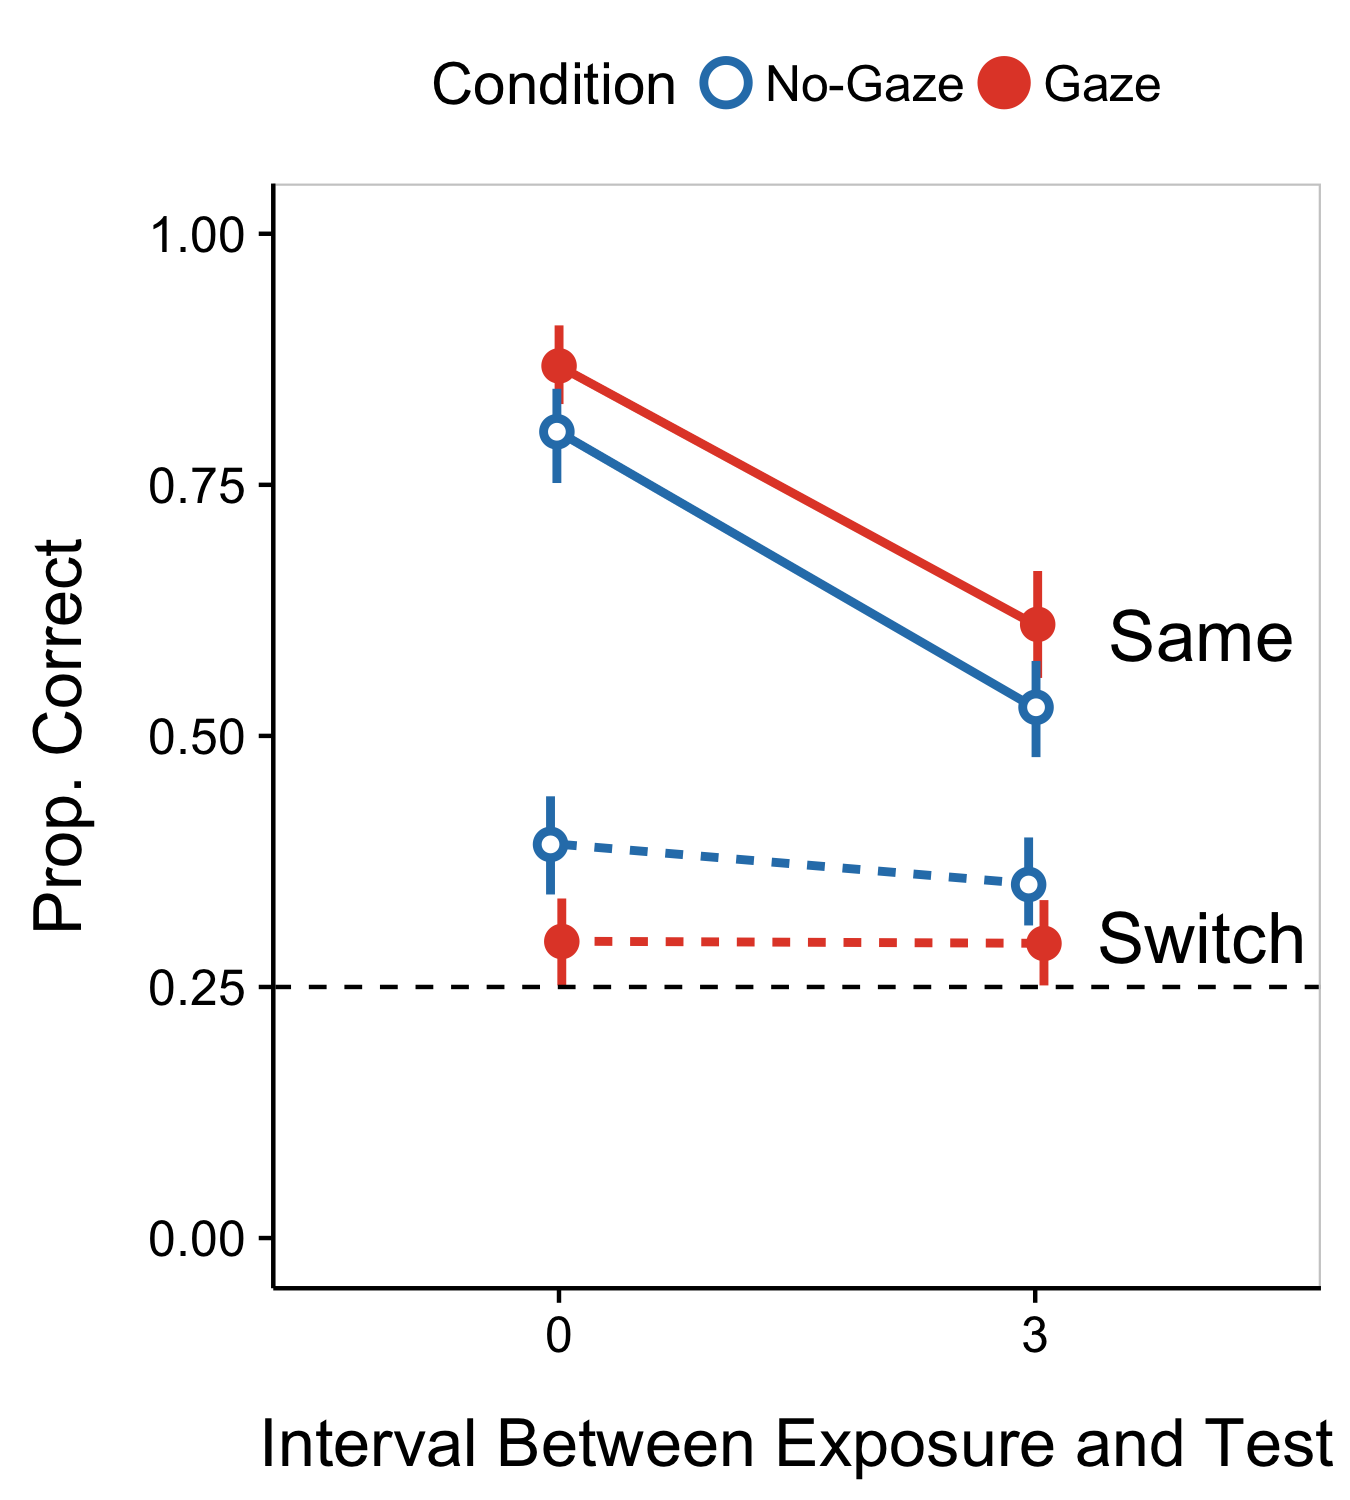
\includegraphics[width=0.5\linewidth]{/Users/ejyoon/Documents/Documents/Research/dissertation/index/chapter_child_rmds/SOC-XSIT/figures/expt4_collapsed} 

}

\caption[Experiment 4.4 results]{Experiment 4.4 results. Accuracy on test trials in Experiment 4 collapsed across the Long and Short inspection time conditions. The dashed line represents chance performance. Color and line type indicate whether there was gaze present on exposure trials. Error bars indicate 95\% confidence intervals computed by non-parametric bootstrap.}\label{fig:expt4-plot}
\end{figure}
We did not see strong evidence of an effect of the different inspection
times. Thus, all of the results reported here collapse across the short
and long inspection time conditions. For all analyses, we removed the
trials on which participants did not respond within the fixed inspection
time on exposure trials (0.05\% of trials).

\subsubsection{Exposure Trials}\label{exposure-trials-3}

Participants' responses on exposure trials differed from those expected
by chance (smallest \(\beta\) = 2.95, z = 38.08, \(p\) \textless{}
.001), suggesting that gaze was again effective in directing
participants' attention. Similar to Experiment 2, participants were
quite likely to use the gaze cue when it was a video of an actress
(\(M_{0-interval}\) = 0.93, \(M_{3-interval}\) = 0.95).

\subsubsection{Test Trials}\label{test-trials-3}

Figure 6 shows performance on test trials in Experiment 4. In the
majority of conditions, participants selected the correct referent at
rates greater than chance (smallest \(\beta\) = 0.2, z = 2.2, \(p\)
\textless{} .05). However, participants' responses were not different
from chance on Switch trials after exposure trials with gaze in the
3-interval condition (\(\beta\) = 0.17, \(p\) = 0.06).

We replicate the key finding from Experiments 1-3: after seeing exposure
trials with gaze, participants were less accurate on Switch trials
(\(\beta\) = 0.9, \(p\) \textless{} .001). Since inspection times were
fixed across the Gaze and No-Gaze conditions, this finding provides
evidence that the presence of a referential cue did more than just
reduce the amount of time participants' spent inspecting the potential
word-object links. In contrast to Experiments 2 and 3, visual inspection
of Figure 6 suggested that the referential cue provided a boost to
accuracy on Same trials. To assess the simple effect of gaze on trial
type, we computed pairwise contrasts using the \emph{lsmeans} package in
R with a Bonferroni correction for multiple comparisons (Lenth, 2016).
Accuracy was higher for Same trials in the Gaze condition (\(\beta\) =
0.49, \(p\) \textless{} .001), but lower for Switch trials (\(\beta\) =
-0.41, \(p\) \textless{} .001). The boost in accuracy on Same trials
differs from Experiments 2 and 3 and suggests that making inspection
times equivalent across conditions allowed the social cue to affect the
strength of learners' memory for their candidate hypothesis.

The results of Experiment 4 help to clarify the effect of gaze on memory
in our task, providing evidence that the presence of a referential cue
did more than just reduce participants' visual inspection time. Instead,
gaze reduced memory for alternative word-object links even when people
had the same opportunity to visually inspect and encode them. We also
found evidence of a boost for learners' memory of their candidate
hypothesis in the gaze condition, an effect that we saw at the higher
number of referents and the longer intervals in Experiment 1, but that
we did not see in Experiments 2 or 3. One explanation for this
difference is that in Experiment 4, since participants' use of gaze was
independent of the length of exposure trials, inspection times in the
gaze condition were longer compared to those in Experiments 1-3. Thus,
it could be that the combination of a gaze cue coupled with the
opportunity to continue attending to the gaze target led to a boost in
performance on Same trials relative to trials without gaze.

\section{General Discussion}\label{general-discussion-1}

Tracking cross-situational word-object statistics allows word learning
to proceed despite the presence of individually ambiguous naming events.
But models of cross-situational learning disagree about how much
information is actually stored in memory, and the input to statistical
learning mechanisms can vary along a continuum of referential
uncertainty from unambiguous naming instances to highly ambiguous
situations. In the current line of work, we explore the hypothesis that
these two factors are fundamentally linked to one another and to the
social context in which word learning occurs. Specifically, we ask how
cross-situational learning operates over social input that varies the
amount of ambiguity in the learning context.

Our results suggest that the representations underlying
cross-situational learning are quite flexible. In the absence of a
referential cue to word meaning, learners tended to store more
alternative word-object links. In contrast, when gaze was present
learners stored less information, showing behavior consistent with
tracking a single hypothesis (Experiments 1 and 2). Learners were also
sensitive to a parametric manipulation of the strength of the
referential cue, showing a graded increase in the tendency to use the
cue as reliability increased, which in turn resulted in a graded
decrease in memory for alternative word-object links (Experiment 3).
Finally, learners stored less information in the presence of gaze even
when they were shown the objects for the same amount of time (Experiment
4).

In Experiments 2 and 3 reduced memory for alternative hypotheses did not
result in a boost to memory for learners' candidate hypothesis. This
pattern of data suggests that the presence of a referential cue
selectively affected one component of the underlying representation: the
number of alternative word-object links, and not the strength of the
learners' candidate hypothesis. However, in Experiments 1 and 4, we did
see some evidence of stronger memory for learners' initial hypothesis in
the presence of gaze: at the higher number of referents and interval
conditions (Experiment 1), and when the length of exposure trials was
equivalent across the Gaze and No-Gaze conditions (Experiment 4). We
speculate that the relationship between the presence of a referential
cue and the strength of learners' candidate hypothesis is modulated by
how the cue interacts with attention. In Experiment 1, gaze may have
provided a boost because, in the absence of gaze, attention would have
been distributed across a larger number of alternatives. And, in
Experiment 4, gaze may have led to better memory because it was coupled
with the opportunity for sustained attention to the gaze target. More
work is needed in order to understand precisely when the presence of
gaze affects this particular component of the representations underlying
cross-situational learning.

In Experiments 1-3, longer inspection times (i.e., more time spent
encoding the word-object links during learning) led to better memory at
test. We did, however, find slightly different interaction effects
across our studies. In Experiment 1, longer inspection times led to
higher accuracy in the No-Gaze condition for both Same and Switch
trials. In Experiment 2, longer inspection times provided a larger boost
to performance on Switch trials compared to Same trials, regardless of
gaze condition. Despite these differences, we speculate that inspection
time played a similar role across these studies: When a social cue was
present, learners' attention was focused and inspection times tended to
be shorter, which led to worse performance on Switch trials (i.e.,
reduced memory for alternative word-object links). Interestingly, in
Experiment 4, we found an effect of social cues on memory for
alternatives even when participants were given the same opportunity to
visually inspect the objects, suggesting that gaze does more than just
modulate visual attention during learning.

\subsection{Relationship to previous
work}\label{relationship-to-previous-work}

Why might a decrease in memory for alternatives fail to increase the
strength of learners' memory for their candidate hypothesis? One
possibility is that participants did not shift their cognitive resources
from the set of alternatives to their single hypothesis, but instead
chose to use the gaze information to reduce inspection time, thus
conserving their resources for future use. Griffiths, Lieder, and
Goodman (2015) formalize this behavior by pushing the rationality of
computational-level models down to the psychological process level. In
their framework, cognitive systems are thought to be adaptive in that
they optimize the use of their limited resources, taking the cost of
computation (e.g., the opportunity cost of time or mental energy) into
account. For example, Vul, Goodman, Griffiths, and Tenenbaum (2014)
showed that as time pressure increased in a decision-making task,
participants were more likely to show behavior consistent with a less
cognitively challenging strategy of matching, rather than with the
globally optimal strategy. In the current work, we found that learners
showed evidence of altering how they allocated cognitive resources based
on the amount of referential uncertainty present during learning,
spending less time inspecting alternative word-object links and reducing
the number of links stored in memory when uncertainty was low.

Our results fit well with recent experimental work that investigates how
attention and memory can constrain infants' statistical word learning.
For example, Smith and Yu (2013) used a modified cross-situational
learning task to show that only infants who disengaged from a novel
object to look at both potential referents were able to learn the
correct word--object mappings. Moreover, Vlach and Johnson (2013) showed
that 16-month-olds were only able to learn from adjacent
cross-situational co-occurrence statistics, and unable to learn from
co-occurrences that were separated in time. Both of these findings make
the important point that only the information that comes into contact
with the learning system can be used for cross-situational word
learning, and this information is directly influenced by the attention
and memory constraints of the learner. These results also add to a large
literature showing the importance of social information for word
learning (P. Bloom, 2002; E. V. Clark, 2009) and to recent work
exploring the interaction between statistical learning mechanisms and
other types of information (Frank, Goodman, \& Tenenbaum, 2009; Koehne
\& Crocker, 2014; C. Yu \& Ballard, 2007). Our findings suggest that
referential cues affect statistical learning by modulating the amount of
information that learners store in the underlying representations that
support learning over time.

Is gaze a privileged cue, or could other, less-social cues (e.g., an
arrow) also affect the representations underlying cross-situational
learning? On the one hand, previous research has shown that gaze cues
lead to more reflexive attentional responses compared to arrows
(Friesen, Ristic, \& Kingstone, 2004), that gaze-triggered attention
results in better learning compared to salience-triggered attention (R.
Wu \& Kirkham, 2010), and that even toddlers readily use gaze to infer
novel word meanings (Baldwin, 1993). Thus, it could be that gaze is an
especially effective cue for constraining word learning since it
communicates a speaker's referential intent and is a particularly good
way to guide attention. On the other hand, the generative process of the
cue -- whether it is more or less social in nature -- might be less
important; instead, the critical factor might be whether the cue
effectively reduces uncertainty in the naming event. Under this account,
gaze is placed amongst a set of many cues that could produce similar
effects as those reported here. Future work could explore a wider range
of cues to see if they modulate the representations underlying
cross-situational learning in a similar way.

How should we characterize the effect of gaze on attention and memory in
our task? One possibility is that the referential cue acts as a filter,
only allowing likely referents to contact statistical learning
mechanisms (C. Yu \& Ballard, 2007). This `filtering account' separates
the effect of social cues from the underlying computation that
aggregates cross-situational information. Another possibility is that
referential cues provide evidence about a speaker's communicative intent
(Frank et al., 2009). In this model, the learner is reasoning about the
speaker and word meanings simultaneously, which places inferences based
on social information as part of the underlying computation. A third
possibility is that participants thought of the referential cue as
pedagogical. In this context, learners assume that the speaker will
choose an action that is most likely to increase the learner's belief in
the true state of the world (Shafto, Goodman, \& Frank, 2012), making it
unnecessary to allocate resources to alternative hypotheses. Experiments
show that children spend less time exploring an object and are less
likely to discover alternative object-functions if a single function is
demonstrated in a pedagogical context (Bonawitz et al., 2011). However,
because the results from the current study cannot distinguish between
these explanations, these questions remain topics for future studies
specifically designed to tease apart these possibilities.

\subsection{Limitations}\label{limitations}

There are several limitations to the current study that are worth
noting. First, the social context that we used was relatively
impoverished. Although we moved beyond a simple manipulation of the
presence or absence of social information in Experiment 3, we
nevertheless isolated just a single cue to reference, gaze. But
real-world learning contexts are much more complex, providing learners
access to multiple cues such as gaze, pointing, and previous discourse.
In fact, Frank, Tenenbaum, and Fernald (2013) analyzed a corpus of
parent-child interactions and concluded that learners would do better to
aggregate noisy social information from multiple cues, rather than
monitor a single cue since no single cue was a consistent predictor of
reference. In our data, we did see a more reliable effect of referential
cues when we used a video of an actress, which included both gaze and
head turn as opposed to the static, schematic stimuli, which only
included gaze. It is still an open and interesting question as to how
our results would generalize to learning environments that contain a
rich combination of social cues.

Second, we do not yet know how variations in referential uncertainty
during learning would affect the representations of young word learners,
the age at which cross-situational word learning might be particularly
important. Recent research using a similar paradigm as our own did not
find evidence that 2- or 3-year-olds stored multiple word-object links;
instead, children only retained a single candidate hypothesis (Woodard,
Gleitman, \& Trueswell, 2016). However, performance limitations on
children's developing attention and memory systems (Colombo, 2001;
Ross-sheehy, Oakes, \& Luck, 2003) could make success on these explicit
response tasks more difficult. Moreover, our work suggests that
different levels of referential uncertainty in naturalistic learning
contexts (see Medina, Snedeker, Trueswell, \& Gleitman, 2011; Yurovsky
\& Frank, 2015) might evoke different strategies for information
storage, with learners retaining more information as ambiguity in the
input increases. Thus, we think that it will be important to test a
variety of outcome measures and learning contexts to see if younger
learners show evidence of storing multiple word meanings during
learning.

In addition, previous work with infants has shown that their attention
is often stimulus-driven and sticky (Oakes, 2011), suggesting that very
young word learners might not effectively explore the visual scene in
order to extract the necessary statistics for storing multiple
alternatives. It could be that referential cues play an even more
important role for young learners by filtering the input to
cross-situational word learning mechanisms and guiding children to the
relevant statistics in the input. In fact, recent work has shown that
the precise timing of features such as increased parent attention and
gesturing towards a named object and away from non-target objects were
strong predictors of referential clarity in a naming event (Trueswell et
al., 2016). It could be that the statistics available in these
particularly unambiguous naming events are the most useful for
cross-situational learning.

Finally, the current experiments used a restricted cross-situational
word learning scenario, which differs from real-world language learning
contexts in several important ways. One, we only tested a single
exposure for each novel word-object pairing; whereas, real-world naming
events are best characterized by discourse where an object is likely to
be named repeatedly in a short amount of time (Frank, Tenenbaum, \&
Fernald, 2013; Rohde \& Frank, 2014). Two, the restricted visual world
of 2-8 objects on a screen combined with the forced-choice response
format may have biased people to assume that all words in the task must
have referred to one of the objects. But, in actual language use, people
can refer to things that are not physically co-present (e.g., Gleitman,
1990), creating a scenario where learners would not benefit from storing
additional word-object links in the absence of clear referential cues.
Finally, we presented novel words in isolation, removing any sentential
cues to word meaning (e.g., verb-argument relations). In fact, previous
work with adults has shown that cross-situational learning mechanisms
only operate in contexts where sentence-level constraints do not
completely disambiguate meaning (Koehne \& Crocker, 2014). Thus, we need
more evidence to understand how the representations underlying
cross-situational learning change in response to referential uncertainty
at different timescales and in richer language contexts that more
accurately reflect real-world learning environments.

\section{Conclusions}\label{conclusions-1}

Word learning proceeds despite the potential for high levels of
referential uncertainty and despite learners' limited cognitive
resources. Our work shows that cross-situational learners flexibly
respond to the amount of ambiguity in the input, and as referential
uncertainty increases, learners tend to store more word-object links.
Overall, these results bring together aspects of social and statistical
accounts of word learning to increase our understanding of how
statistical learning mechanisms operate over fundamentally social input.

\chapter{Integrating statistical and social information during language
comprehension and word
learning}\label{integrating-statistical-and-social-information-during-language-comprehension-and-word-learning}

\chaptermark{Seeking social information during language processing}

In this chapter, I present three studies that explore how the presence
of a social cue to reference (a speaker's gaze) changes listeners'
decisions about visual fixation during language comprehension and word
learning. Within our broader active-social framework, these studies ask
how the value of information gained from fixating on (i.e., querying) a
social partner interacts with learners' developing knowledge of word
meanings (i.e., hypotheses) to modulate their information accumulation
thresholds (i.e., stopping rules). This work brings together the core
elements -- active, social, and statistical -- of the integrative
account described in Chapter 1.

Children process language in complex environments where there are often
many things to talk about. How do they understand and learn words
despite this noisy input? Statistical learning accounts emphasize that
children can aggregate consistent word-object co-occurrences across
multiple labeling events to reduce uncertainty over time.
Social-pragmatic theories argue that interactions with social partners
support learning by reducing ambiguity within individual labeling
events. Here, we present three eye-tracking studies that ask how
children integrate statistical and social information during real-time
language processing. First, children and adults did not delay their gaze
shifts to gather a post-nominal social cue to reference (another
speaker's eye gaze). Second, when processing novel words, adults fixated
more on a speaker who provided a disambiguating gaze and showed stronger
recall for word-object links learned via the social cue. Finally, in
contrast to the familiar word context, children and adults fixated
longer on a speaker who produced a gaze cue when labeling novel objects,
which, in turn, led to increased looking to the named object and less
looking to the other objects in the scene. Moreover, children, but not
adults, increased their looking to the interlocutor throughout the
experiment. Together, these results suggest that learners flexibly
integrate their knowledge of object labels to decide whether to seek
social information, which then shapes the information that comes into
contact with statistical learning mechanisms.

\chapter*{Conclusion}\label{conclusion}
\addcontentsline{toc}{chapter}{Conclusion}

In this dissertation, I proposed a framework for understanding
children's information-seeking decisions within social contexts. The
core of the argument is that the presence of other people can change the
\emph{availability} and \emph{usefulness} of information-seeking
behaviors by shaping learners' goals, hypotheses, actions, answers, and
thresholds for stopping information gathering. Following the theoretical
framework, I presented a set of empirical studies that explored whether
the dynamics of children's real-time information selection via their eye
movements flexibly adapts to gather social information that supports
language processing.

Chapter 2 investigated how children learning American Sign Language
(ASL) distributed visual attention between the linguistic signal and
referents, which both compete for visual attention. Similar to children
learning spoken language, ASL learners shifted gaze away from a social
partner to seek objects before sign offset, providing evidence that,
despite channel competition, language drove rapid shifts in visual
attention to named referents. Chapter 3 extended the sign language
research by directly comparing ASL learners' gaze dynamics to those of
children learning spoken English using parallel real-time language
comprehension tasks. Chapter 3 also presented a comparison of
English-learning children and adults' eye movements in noisy vs.~clear
auditory contexts. In both the ASL and noisy speech cases, listeners
adapted their gaze to seek additional language-relevant information from
social partners before shifting to seek a named referent. Chapters 4 and
5 explored how eye movements change when children and adults processed
familiar and novel words accompanied by social cues to reference. Taken
together, the social gaze work suggests that children integrate their
uncertainty over word-object mappings to decide when to seek social
information, which in turn, modulates the input to statistical word
learning.

The integrative framework and empirical work described here are limited
in several important ways. First, the majority of this research tested
binary hypotheses of behavior change -- i.e., sign vs.~spoken language;
noisy vs.~clear speech; word learning with vs.~without social gaze -- to
answer the question of whether children would flexibly adapt their
information seeking in response to changes in their processing
environments. Chapters 2-5 present evidence across a diverse set of case
studies that children's real-time information seeking is quite flexible.
However, to move the integrative framework forward, we would want to
develop a fully-specified model that could make quantitative predictions
about how social contexts will change the utility of information-seeking
behaviors. This step will require formalizing the notions of value and
cost of information-seeking actions in a modeling framework that can
incorporate the effects of reasoning about other people's mental states.

We have taken some initial steps towards this goal by developing a model
of active-social learning that integrates ideas from Optimal Experiment
Design (OED) with formalizations of recursive social reasoning from
Bayesian models of pragmatic language interpretation (N. D. Goodman \&
Frank, 2016b). We found that this integrated model was able to reproduce
the qualitative patterns in adults' decisions of whether to forego
information seeking in favor of more immediately rewarding actions when
their social partner highlighted performance and presentational goals
(Erica J Yoon, MacDonald, Asaba, Gweon, \& Frank, 2018). The integrative
framework described here directly inspired this line of research, and I
hope that future versions of the model will be able to generate graded,
testable predictions for behavior across a variety of domains -- e.g.,
eye movements, early vocalizations, and verbal question asking.

Second, we used one particular formalization of active inquiry. The OED
model focuses on learners' information-seeking decisions given a
specific goal to learn and a set of candidate hypotheses. Other
computational frameworks have formalized active learning in different
ways. For example, foraging models pursue the analogy that human
information seeking is similar to animals' decisions about where and how
long to look for food if they were trying to maximize caloric intake
while minimizing their effort and time (see Pirolli \& Card (1999) for a
review). Cognitive scientists have successfully modeled a range of
behaviors as a form of spatial foraging, such as searching for semantic
concepts in memory (Hills, Jones, \& Todd, 2012) and decisions about
where to direct visual attention in real-time (Manohar \& Husain, 2013).
In addition to these search models, recent work on curiosity-based
learning in developmental robotics has created algorithms that optimize
intrinsic estimates of learning progress. This formalization creates
systems that focus on seeking activities and stimuli of intermediate
complexity where learners' predictions are steadily improving, and
uncertainty is steadily decreasing (Oudeyer \& Smith, 2016). One of the
challenges for researchers trying to integrate active and social
learning is that the space of possible connections is quite large. By
constraining our framework to active decision making, we were able to
make some progress on an important sub-component of a larger set of
children's information-seeking behaviors. Future theoretical work,
however, should consider possible connections between social learning
phenomena and the foraging/curiosity-based learning frameworks.

Third, our ultimate goal for the active-social framework is to
incorporate effects at a developmental timescale. The experiments in
this thesis, however, often treated children and adults as two endpoints
on a continuum, exploring parallels and differences between children's
information seeking and our best estimate of the mature state of the
language processing system. We did find some clear patterns of
developmental change. In Chapter 3, adults were faster to respond to
familiar words, generated more language-consistent shifts, and produced
fewer early shifts before accumulating enough information. Older
children were also faster to respond than younger children but did not
generate more language-consistent shifts overall. Older children did,
however, produce fewer early, non-language-driven gaze shifts. This
pattern of results suggests that what might be developing is an ability
to inhibit a behavior -- shifting gaze away from the language source --
that reduces access to information that is useful for figuring out the
identity of a named referent. Prior work also shows that children
develop greater flexibility in ignoring irrelevant information to focus
on parts of the meaningful parts of a sentence (Zangl \& Fernald, 2007).
But it is still an open question as to how children's visual information
seeking might change as they become more efficient in processing words
and develop their skill in focusing on relevant information in their
environment.

In addition to change at the developmental timescale, the final
experiment in Chapter 5 represents an exception where we measured
adaptation of information seeking over the slightly longer timescale of
multiple exposures to novel word-object links and in the context of
highly familiar words, which children learned through exposure to many
prior labeling events in their day-to-day lives. While the study in
Chapter 5 is a useful first step, future work should measure change over
a longer timescale by densely sampling children at different ages and
points of development. For example, it would be useful to know the
effect of children's rapidly improving productive language skills, which
increases the set of information-seeking actions available by allowing
children to ask verbal questions. One prediction based on our framework
is that seeking social information via eye movements should become less
useful when children can produce the verbal question ``What is this
thing called?'' since it has a higher probability of returning useful
information. Another example is children's rapid theory of mind
development. Our framework predicts that young children should focus
more on learning goals if they are less skilled at reasoning about
others' beliefs. But, as their social reasoning abilities mature and
their social environments become more complex, children may forego
information seeking actions that make them appear incompetent to their
social partners.

Fourth, our account is currently underdeveloped concerning individual
differences. That is, the model was designed to explore general
principles about how qualitative changes to the social environment might
shape children's information seeking actions. However, it is possible to
use the active-social framework to understand how individual differences
in children's input and cognitive abilities might interact to shape how
they decide to seek information from social partners. For example, prior
research has found that adults vary in the proportion of unambiguous
naming episodes they provide, with some parents rarely providing highly
informative contexts and others' doing so relatively more often
(Cartmill et al., 2013). Within our active-social framework, this
differential experience could be instantiated as children learning a
model of the probability of getting a high-quality answer when they ask
a question. If children do not expect an answer is likely, then this
should reduce information seeking even if there is a social partner
available. We did find some evidence of this effect in Chapters 4 and 5
where adults were less likely to use an unreliable social cue to
reference and where children looked more to a social partner who
provided gaze cue than to one who did not.

Individual differences in cognitive abilities could also be included in
our model. Prior research shows variability in children's theory of mind
and inhibitory control abilities (Carlson \& Moses, 2001), in addition
to the considerable variability in language processing skill (Marchman
\& Fernald, 2008). Within our active-social framework, children with a
more-developed theory of mind skill might place a higher weight on
pursuing social goals over and above informational goals, taking actions
that maintain others' beliefs about their abilities. It could also be
that stronger perspective-taking skills help children reason about the
probability of getting a quality answer from another person, thus
modulating whom they choose to ask questions (e.g., seeking information
from an expert vs.~a novice). Another compelling possibility is that
children who have stronger domain-general processing abilities are
better able to update their beliefs based on the information they
receive, and thus reducing the amount of time they spend seeking
information from social partners. These are all interesting, open
questions for future research that fall out of the integrative
active-social framework proposed in this thesis.

Finally, the empirical research described here aimed to understand how
children's information-seeking behaviors adapt to support their language
processing. To accomplish this, we measured changes in children's gaze
dynamics during language comprehension and word learning in simplified
environments. This approach has the benefit of providing a high degree
of experimenter control and a relatively well-understood hypothesis
linking observable behavior (eye movements) to underlying psychological
constructs (e.g., lexical access) (Tanenhaus, Magnuson, Dahan, \&
Chambers, 2000). The risk, however, is that the responses that we can
measure in the lab do not reflect behaviors that support children's
learning in their natural environments. That is, children acquire their
first language from conversations where social partners produce
contingent responses and take actions that control the flow of
children's learning experience. This gap suggests two critical next
steps for the research described here: (1) measure changes in children's
information seeking within free-flowing social interactions with their
caregivers (see Franchak, Kretch, \& Adolph (2018) for a recent example
of this approach using head-mounted eye trackers), and (2) develop more
realistic lab-based experiments that incorporate behaviorally-relevant
features of children's learning environments such as contingent
responding to children's actions (see Benitez \& Saffran (2018) for an
example of studying word learning using a gaze-contingent eye-tracking
paradigm).

In sum, we set out to explore how children's eye movements adapt to a
wide range of social contexts during two ecologically-relevant tasks:
familiar language comprehension and novel word learning. We found that
children could adapt their gaze to seek relevant social information when
it was useful for language processing. Moreover, children and adults
showed evidence of differential learning of new words when social gaze
guided their visual attention. This work highlighted two critical, open
challenges for a framework of information-seeking within social
contexts: (1) develop a precise quantitative model of how social
learning can change the utility of information-seeking behaviors, and
(2) move beyond highly-constrained lab experiments to document
information seeking behaviors in children's natural learning
environments. Despite these challenges, the integrative framework
presented in this thesis represents a way forward for understanding how
children's information seeking adapts to the wide variety of social
environments in which children acquire their first language.

\appendix

\chapter{Supplementary materials for Chapter
2}\label{supplementary-materials-for-chapter-2}

In this appendix, we present FIXME.

\section{Model details}\label{model-details}

The \emph{literal listener} \(L_0\) is a simple Bayesian agent that
takes the utterance to be true:

\[P_{L_0}(s | w) \propto [\![ w ]\!] (s) * P(s).\]

\noindent where \([\![ w ]\!](s)\) is the truth-functional denotation of
the utterance \(w\) (i.e.~the utterance's literal meaning): It is a
function that maps world-states \(s\) to Boolean truth values. The
literal meaning is used to update the literal listener's prior beliefs
over world states \(P(s)\).

The \emph{speaker} \(S_1\) chooses utterances approximately optimally
given a utility function, which can be decomposed into two components.
First, informational utility (\(U_{inf}\)) is the amount of information
a literal listener \(L_0\) would still not know about world state \(s\)
after hearing a speaker's utterance \(w\). Second, social utility
(\(U_{soc}\)) is the expected subjective utility of the state inferred
given the utterance \(w\). The utility of an utterance subtracts the
cost \(c(w)\) from the weighted combination of the social and epistemic
utilities.

\[U(w; s; \phi_{S_1}) = \phi_{S_1} \cdot \ln(P_{L_0}(s \mid w)) + (1 - \phi_{S_1}) \cdot \mathbb{E}_{P_{L_0}(s \mid w)}[V(s)] - C(w).\]

\noindent The speaker then chooses utterances \(w\) softmax-optimally
given the state \(s\) and his goal weight mixture \(\phi_{S_1}\):

\[P_{S_1}(w \mid s, \phi_{S_1}) \propto \mathrm{exp}(\lambda_{1} \cdot \mathbb{E}[U(w; s; \phi_{S_1})]).\]

\section{Literal semantic task}\label{literal-semantic-task}

We probed judgments of literal meanings of the target words assumed by
our model and used in our main experiment.

\subsection{Participants}\label{participants-8}

51 participants with IP addresses in the United States were recruited on
Amazon's Mechanical Turk.

\subsection{Design and Methods}\label{design-and-methods-1}

We used thirteen different context items in which a speaker evaluated a
performance of some kind. For example, in one of the contexts, Ann saw a
presentation, and Ann's feelings toward the presentation (true state)
were shown on a scale from zero to three hearts (e.g., two out of three
hearts filled in red color; see Figure~\ref{fig:screenshot} for an
example of the heart scale). The question of interest was ``Do you think
Ann thought the presentation was / wasn't X?'' and participants
responded by choosing either ``no'' or ``yes.'' The target could be one
of four possible words: \emph{terrible}, \emph{bad}, \emph{good}, and
\emph{amazing}, giving rise to eight different possible utterances (with
negation or no negation). Each participant read 32 scenarios, depicting
every possible combination of states and utterances. The order of
context items was randomized, and there were a maximum of four repeats
of each context item per participant.

\subsection{Behavioral results}\label{behavioral-results-1}

We analyzed the data by collapsing across context items. For each
utterance-state pair, we computed the posterior distribution over the
semantic weight (i.e., how consistent X utterance is with Y state)
assuming a uniform prior over the weight (i.e., a standard Beta-Binomial
model). Meanings of the words as judged by participants were as one
would expect (Figure~\ref{fig:litsem}).
\begin{figure}[!h]

{\centering 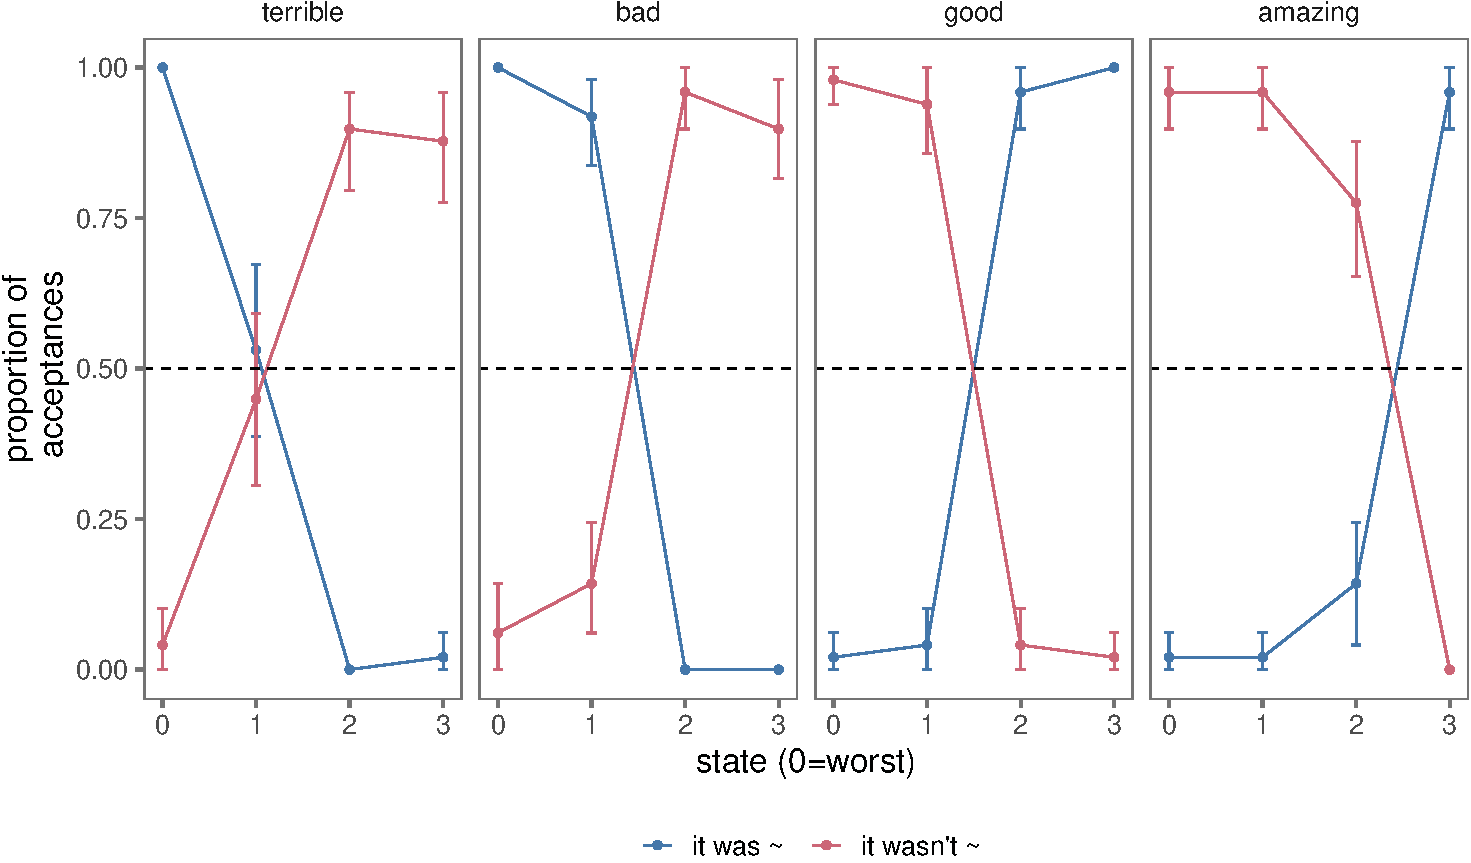
\includegraphics[width=\textwidth]{erica_yoon_dissertation_files/figure-latex/litsem-1} 

}

\caption{Semantic measurement results. Proportion of acceptances of utterance types (shown in different colors) combined with target words (shown in different facets) given the true state represented on a scale of hearts. Error bars represent 95\% confidence intervals.}\label{fig:litsem}
\end{figure}
\section{Data analysis}\label{data-analysis}

We used R (Version 3.4.3; R Core Team, 2017) and the R-packages
\emph{BayesFactor} (Version 0.9.12.2; Morey \& Rouder, 2015),
\emph{bindrcpp} (Version 0.2.2; Müller, 2017a), \emph{binom} (Version
1.1.1; Dorai-Raj, 2014), \emph{brms} (Version 2.0.1; Bürkner, 2017),
\emph{coda} (Version 0.19.1; Plummer, Best, Cowles, \& Vines, 2006),
\emph{directlabels} (Version 2017.3.31; Hocking, 2017), \emph{dplyr}
(Version 0.8.0.1; Wickham, Francois, Henry, \& Müller, 2017),
\emph{forcats} (Version 0.2.0; Wickham, 2017a), \emph{ggplot2} (Version
3.0.0; Wickham, 2009), \emph{ggthemes} (Version 3.4.0; Arnold, 2017),
\emph{gridExtra} (Version 2.3; Auguie, 2017), \emph{here} (Version 0.1;
Müller, 2017b), \emph{jsonlite} (Version 1.6; Ooms, 2014),
\emph{langcog} (Version 0.1.9001; Braginsky, Yurovsky, \& Frank, n.d.),
\emph{lme4} (Version 1.1.15; D. Bates, Mächler, Bolker, \& Walker,
2015), \emph{magrittr} (Version 1.5; Bache \& Wickham, 2014),
\emph{Matrix} (Version 1.2.12; D. Bates \& Maechler, 2017),
\emph{papaja} (Version 0.1.0.9655; Aust \& Barth, 2017), \emph{purrr}
(Version 0.2.5; Henry \& Wickham, 2017), \emph{RColorBrewer} (Version
1.1.2; Neuwirth, 2014), \emph{Rcpp} (Eddelbuettel \& Balamuta, 2017;
Version 1.0.1; Eddelbuettel \& François, 2011), \emph{readr} (Version
1.1.1; Wickham, Hester, \& Francois, 2017), \emph{rwebppl} (Version
0.1.97; Braginsky, Tessler, \& Hawkins, n.d.), \emph{stringr} (Version
1.3.1; Wickham, 2017b), \emph{tibble} (Version 2.1.1; Müller \& Wickham,
2017), \emph{tidyr} (Version 0.7.2; Wickham \& Henry, 2017), and
\emph{tidyverse} (Version 1.2.1; Wickham, 2017c) for all our analyses.

\section{Full statistics on human
data}\label{full-statistics-on-human-data}
\begin{table}[tbp]
\begin{center}
\begin{threeparttable}
\caption{\label{tab:brmTab}Predictor mean estimates with standard deviation and 95\% credible interval information for a Bayesian linear mixed-effects model predicting negation production based on true state and speaker goal (with both-goal as the reference level).}
\begin{tabular}{lllll}
\toprule
Predictor & \multicolumn{1}{c}{Mean} & \multicolumn{1}{c}{SD} & \multicolumn{1}{c}{95\% CI-Lower} & \multicolumn{1}{c}{95\% CI-Upper}\\
\midrule
Intercept & 0.88 & 0.13 & 0.63 & 1.12\\
True state & 2.18 & 0.17 & 1.86 & 2.53\\
Goal: Informative & 0.47 & 0.17 & 0.14 & 0.80\\
Goal: Kind & 0.97 & 0.25 & 0.51 & 1.49\\
True state * Informative & -1.33 & 0.18 & -1.69 & -0.98\\
True state * Kind & -0.50 & 0.22 & -0.92 & -0.07\\
\bottomrule
\end{tabular}
\end{threeparttable}
\end{center}
\end{table}
We used Bayesian linear mixed-effects models (\texttt{brms} package in
R; Bürkner, 2017) using crossed random effects of true state and goal
with maximal random effects structure (Barr et al., 2013b; A. Gelman \&
Hill, 2006). The full statistics are shown in Table \ref{tab:brmTab}.

\section{Model fitting and inferred
parameters}\label{model-fitting-and-inferred-parameters}
\begin{table}[tbp]
\begin{center}
\begin{threeparttable}
\caption{\label{tab:otherParams}Inferred negation cost and speaker optimality parameters for all model variants.}
\begin{tabular}{lll}
\toprule
Model & \multicolumn{1}{c}{Cost of negation} & \multicolumn{1}{c}{Speaker optimality}\\
\midrule
ninformational only & 1.58 & 8.58\\
ninformational, presentational & 1.89 & 2.93\\
ninformational, social & 1.11 & 3.07\\
ninformational, social, presentational & 2.64 & 4.47\\
presentational only & 2.58 & 9.58\\
social only & 1.73 & 7.23\\
social, presentational & 2.49 & 5.29\\
\bottomrule
\end{tabular}
\end{threeparttable}
\end{center}
\end{table}
Other than speaker goal mixture weights explained in the main text
(shown in Table \ref{tab:phi}), the full model has two global
parameters: the speaker's soft-max parameter \(\lambda_{S_2}\) and
soft-max paramater of the hypothetical speaker that the pragmatic
listener reasons about \(\lambda_{S_1}\). \(\lambda_{S_1}\) was 1, and
\(\lambda_{S_2}\) was inferred from the data: We put a prior that was
consistent with those used for similar models in this model class:
\(\lambda_{S_2}\) \textasciitilde{} \(Uniform(0,20)\). Finally, we
incorporate the literal semantics data into the RSA model by maintaining
uncertainty about the semantic weight of utterance \(w\) for state
\(s\), for each of the states and utterances, and assuming a
Beta-Binomial linking function between these weights and the literal
semantics data (see \emph{Literal semantics task} above). We infer the
posterior distribution over all of the model parameters and generate
model predictions based on this posterior distribution using Bayesian
data analysis (M. D. Lee \& Wagenmakers, 2014). We ran 4 MCMC chains for
80,000 iterations, discarding the first 40,000 for burnin. The inferred
values of parameters are shown in Table \ref{tab:otherParams}.

\section{Data Availability}\label{data-availability}

Our model, preregistration of hypotheses, procedure, data, and analyses
are available at \url{https://github.com/ejyoon/polite_speaker}.

\section{Supplemental Figures}\label{supplemental-figures}
\begin{figure}[!h]

{\centering 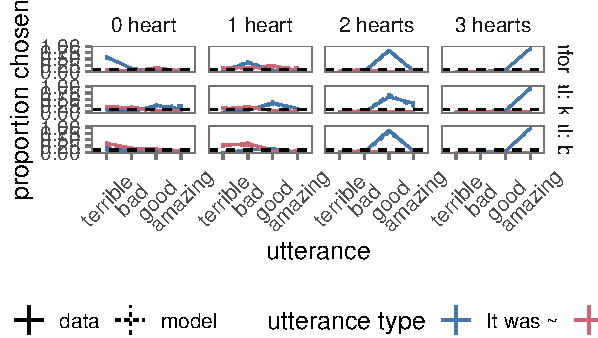
\includegraphics[width=\textwidth]{erica_yoon_dissertation_files/figure-latex/utterance-1} 

}

\caption{Experimental results (solid lines) and fitted predictions from the full model (dashed lines) for speaker production. Proportion of utterances chosen (utterance type – direct vs. indirect – in different colors and words shown on x-axis) given the true states (columns) and speaker goals (rows). Error bars represent 95\% confidence intervals for the data and 95\% highest density intervals for the model. Black dotted line represents the chance level.}\label{fig:utterance}
\end{figure}
\begin{figure}[!h]

{\centering 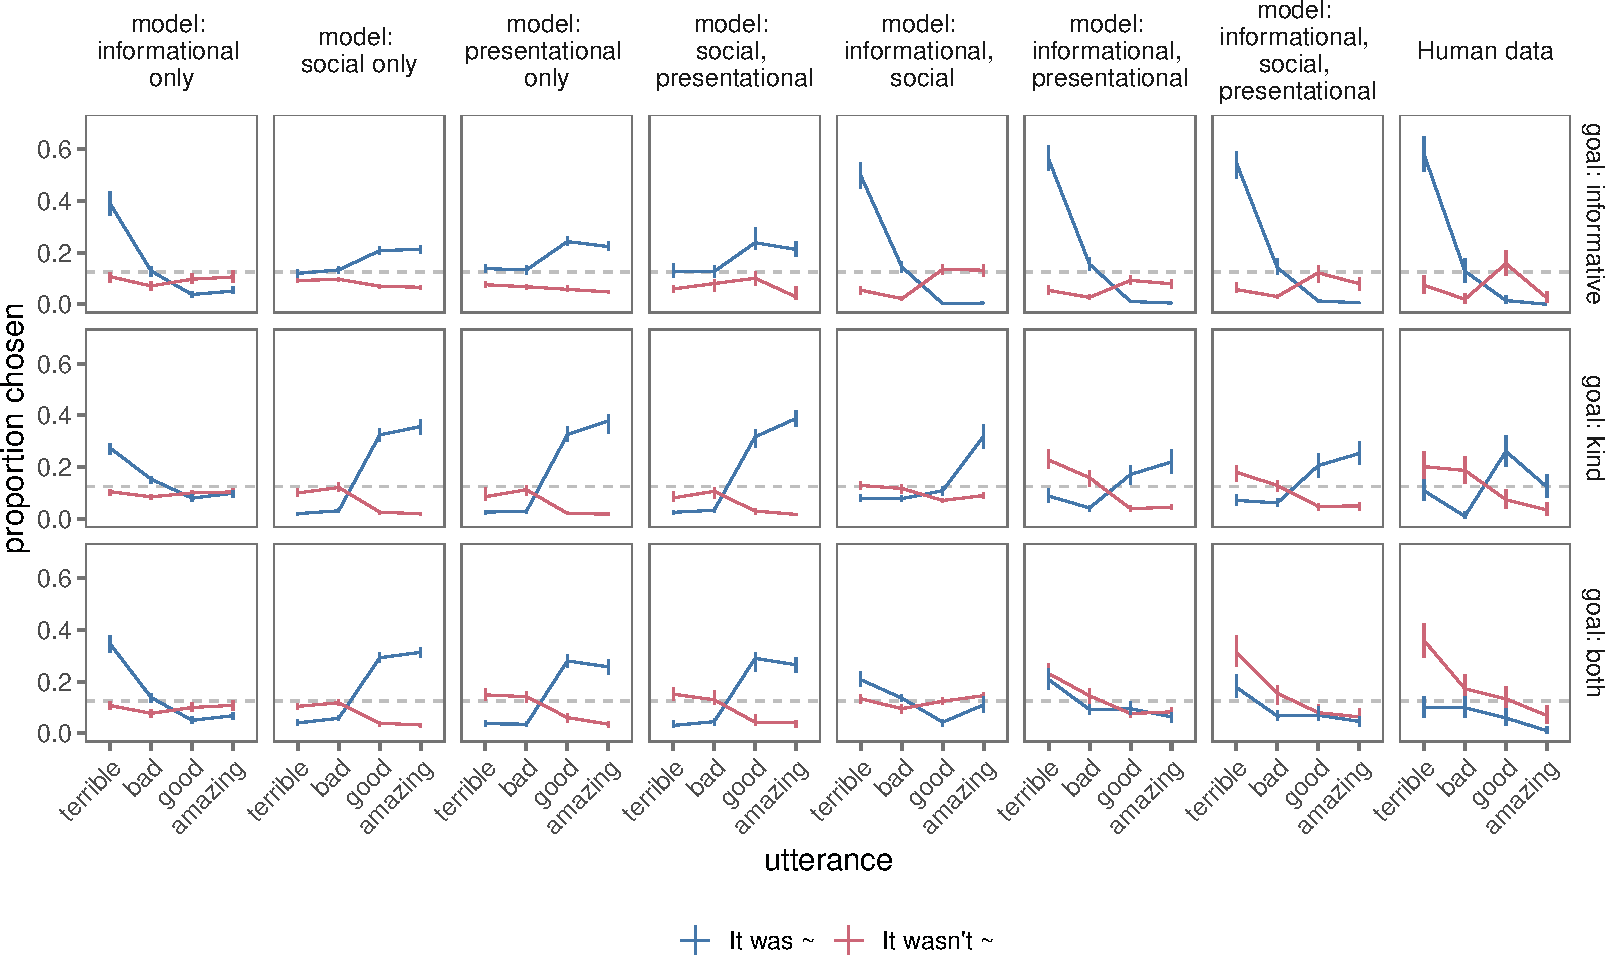
\includegraphics[width=\textwidth]{erica_yoon_dissertation_files/figure-latex/comparisonAll-1} 

}

\caption{Comparison of predictions for proportion of utterances chosen by pragmatic speaker from possible model variants (left) and human data (rightmost) for average proportion of negation produced among all utterances, given true state of 0 heart and speaker with a goal to be informative (top), kind (middle), or both (bottom). Gray dotted line indicates chance level at 12.5\%.}\label{fig:comparisonAll}
\end{figure}
\begin{figure}[!h]

{\centering 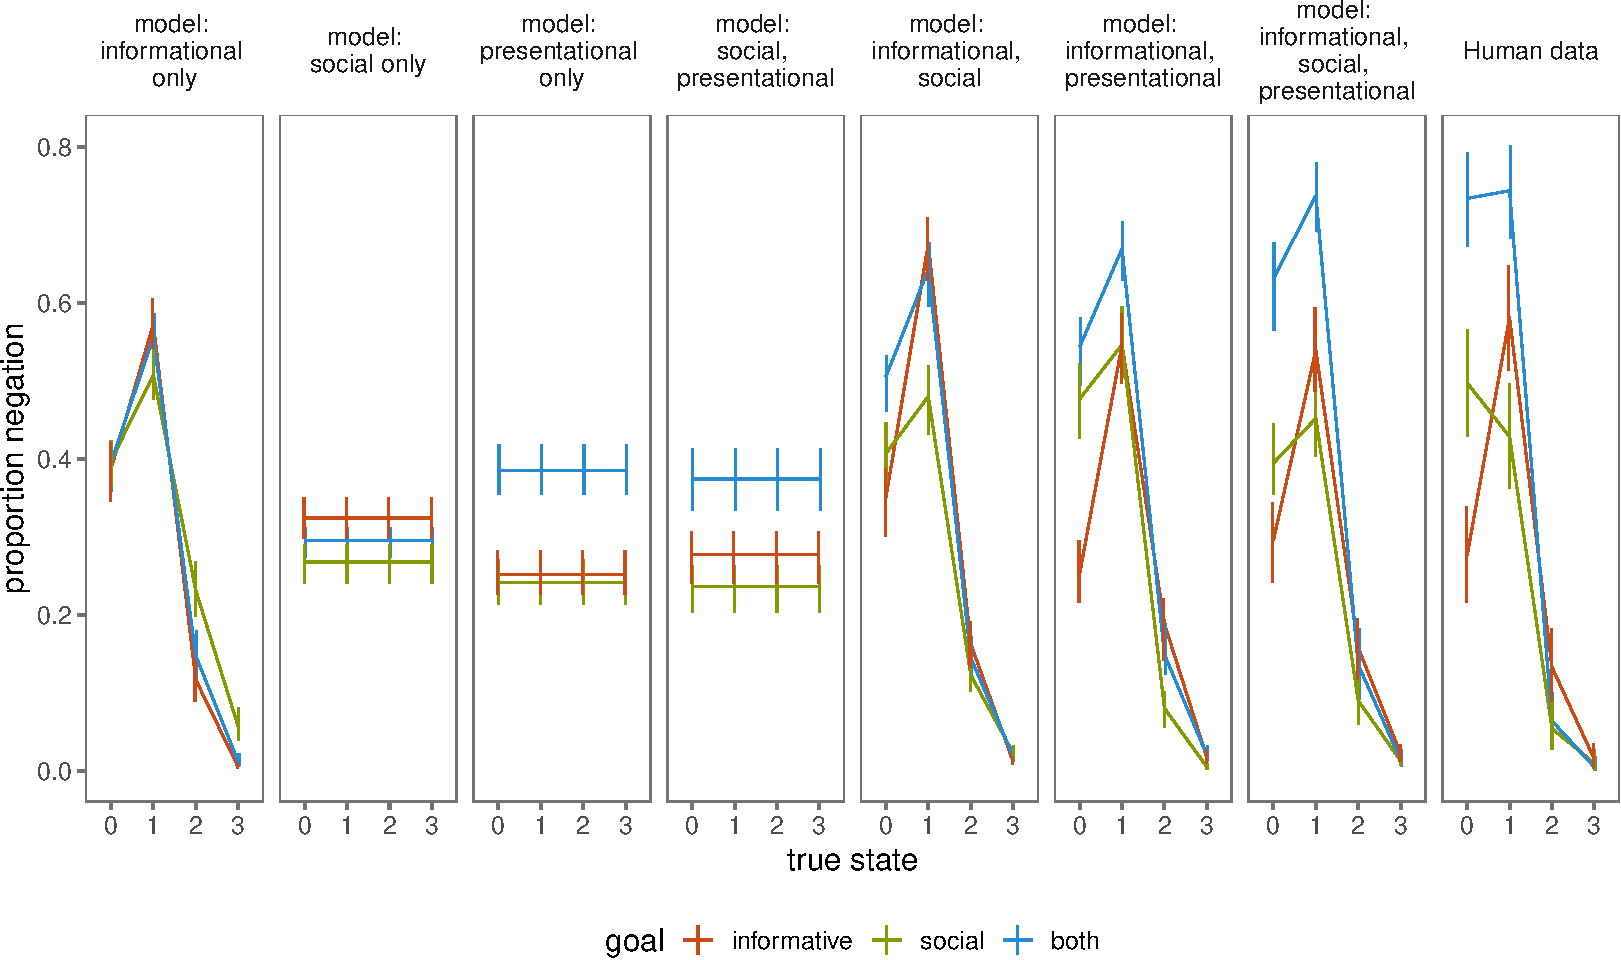
\includegraphics[width=\textwidth]{erica_yoon_dissertation_files/figure-latex/negation-1} 

}

\caption{Experimental results (left) and fitted model predictions (right) for average proportion of negation produced among all utterances, given true states (x-axis) and goals (colors).}\label{fig:negation}
\end{figure}
\chapter{Supplementary materials for Chapter
3}\label{supplementary-materials-for-chapter-3}

\section{Model output for Experiment
3.1}\label{model-output-for-experiment-3.1}

\section{Model output for Experiment
3.2}\label{model-output-for-experiment-3.2}

\chapter{Supplementary materials for Chapter
4}\label{supplementary-materials-for-chapter-4}

\section{Analytic model specifications and
output}\label{analytic-model-specifications-and-output}

\subsection{Experiment 1}\label{experiment-1-2}

\captionsetup[table]{labelformat=empty}

\section*{Table A1. Length of inspection times on exposure trials in Experiment 1 as a function of gaze, interval, and number of referents}

\texttt{Log(Inspection time) $\sim$ (Gaze + Log(Interval) + Log(Referents))$^2$ + (1 | subject)}
\begin{table}[h]
\centering
\begin{tabular}{lrrrrl}
 term & estimate & std.error & t.value & p.value &  \\ 
  \hline
Intercept & 0.83 & 0.10 & 8.19 & $<$ .001 & *** \\ 
  Gaze Condition & 0.16 & 0.11 & 1.48 & 0.138 &  \\ 
  Log(Interval) & 0.06 & 0.05 & 1.33 & 0.184 &  \\ 
  Log(Referents) & 0.34 & 0.04 & 7.91 & $<$ .001 & *** \\ 
  Gaze Condition*Log(Interval) & -0.08 & 0.03 & -2.86 & 0.004 & ** \\ 
  Gaze Condition*Log(Referent) & -0.27 & 0.04 & -6.01 & $<$ .001 & *** \\ 
  Log(Interval)*Log(Referent) & -0.00 & 0.02 & -0.19 & 0.849 &  \\ 
   \hline
\end{tabular}
\label{tab:e1_rt}
\end{table}
\newpage

\section*{Table A2. Accuracy on test trials in Experiment 1 with inspection times on exposure trials included as a predictor}

\texttt{Correct $\sim$ (Trial Type + Gaze + Log(Interval) + Log(Referents) + \\ Log(Inspection Time))$^2$ + offset(logit($^1/_{Referents}$)) + (TrialType | subject)}
\begin{table}[h]
\centering
\begin{tabular}{lrrrrl}
 term & estimate & std.error & z.value & p.value &  \\ 
  \hline
Intercept & 2.89 & 0.34 & 8.49 & $<$ .001 & *** \\ 
  Switch Trial & -1.45 & 0.25 & -5.76 & $<$ .001 & *** \\ 
  Gaze Condition & 0.12 & 0.27 & 0.43 & 0.669 &  \\ 
  Log(Interval) & -0.47 & 0.11 & -4.15 & $<$ .001 & *** \\ 
  Log(Referents) & 0.05 & 0.14 & 0.39 & 0.693 &  \\ 
  Log(Inspection Time) & 0.20 & 0.15 & 1.38 & 0.169 &  \\ 
  Switch Trial*Gaze Condition & -1.02 & 0.13 & -7.86 & $<$ .001 & *** \\ 
  Switch Trial*Log(Interval) & 0.52 & 0.06 & 9.39 & $<$ .001 & *** \\ 
  Switch Trial*Log(Referent) & -0.62 & 0.09 & -6.67 & $<$ .001 & *** \\ 
  Switch Trial*Log(Inspection Time) & 0.09 & 0.07 & 1.36 & 0.174 &  \\ 
  Gaze Condition*Log(Interval) & 0.09 & 0.06 & 1.61 & 0.107 &  \\ 
  Gaze Condition*Log(Referent) & 0.36 & 0.10 & 3.68 & $<$ .001 & *** \\ 
  Gaze Condition*Log(Inspection Time) & -0.17 & 0.07 & -2.55 & 0.011 & * \\ 
  Log(Interval)*Log(Referent) & -0.05 & 0.04 & -1.26 & 0.207 &  \\ 
  Log(Interval)*Log(Inspection Time) & 0.02 & 0.03 & 0.54 & 0.589 &  \\ 
  Log(Referents)*Log(Inspection Time) & 0.05 & 0.05 & 0.94 & 0.345 &  \\ 
   \hline
\end{tabular}
\label{tab:e1_acc_it}
\end{table}
\newpage

\subsection{Experiment 2}\label{experiment-2-2}

\section*{Table A3. Length of inspection times on exposure trials in Experiment 2 as a function of gaze and interval}

\texttt{Log(Inspection time) $\sim$ Gaze * Log(Interval) + (1 | subject)}
\begin{table}[h]
\centering
\begin{tabular}{lrrrrl}
 term & estimate & std.error & t.value & p.value &  \\ 
  \hline
Intercept & 3.90 & 0.08 & 50.69 & $<$ .001 & *** \\ 
  Gaze Condition & -1.10 & 0.05 & -20.90 & $<$ .001 & *** \\ 
  Log(Interval) & -0.48 & 0.05 & -8.77 & $<$ .001 & *** \\ 
  Gaze Condition*Log(Interval) & -0.02 & 0.04 & -0.60 & 0.549 &  \\ 
   \hline
\end{tabular}
\label{tab:e2_rt}
\end{table}
\section*{Table A4. Accuracy on test trials in Experiment 2 with inspection times on exposure trials included as a predictor}

\texttt{Correct $\sim$ (Trial Type + Gaze + Log(Interval) + Log(Inspection Time))$^2$ + \\ offset(logit($^1/_{Referents}$)) + (TrialType | subject)}
\begin{table}[h]
\centering
\begin{tabular}{lrrrrl}
 term & estimate & std.error & z.value & p.value &  \\ 
  \hline
Intercept & 3.51 & 0.29 & 12.13 & $<$ .001 & *** \\ 
  Gaze Condition & 0.13 & 0.23 & 0.58 & 0.559 &  \\ 
  Switch Trial & -3.12 & 0.26 & -12.21 & $<$ .001 & *** \\ 
  Log(Interval) & -0.88 & 0.14 & -6.34 & $<$ .001 & *** \\ 
  Log(Inspection Time) & 0.15 & 0.13 & 1.14 & 0.255 &  \\ 
  Switch Trial*Gaze Condition & -0.54 & 0.17 & -3.21 & 0.001 & ** \\ 
  Gaze Condition*Log(Interval) & 0.16 & 0.09 & 1.85 & 0.064 & . \\ 
  Gaze Condition*Log(Inspection Time) & -0.14 & 0.10 & -1.37 & 0.172 &  \\ 
  Switch Trial*Log(Interval) & 0.77 & 0.10 & 8.00 & $<$ .001 & *** \\ 
  Switch Trial*Log(Inspection Time) & 0.21 & 0.11 & 1.96 & 0.05 & . \\ 
  Log(Interval)*Log(Inspection Time) & 0.04 & 0.06 & 0.77 & 0.44 &  \\ 
   \hline
\end{tabular}
\label{tab:e2_acc_it}
\end{table}
\newpage

\subsection{Experiment 3}\label{experiment-3-3}

\section*{Table A5. Accuracy on exposure trials in Experiment 3 as a function of reliability condition and participants' subjective reliability judgments}

\texttt{Correct-Exposure $\sim$ Reliability Condition * Subjective Reliability + \\  offset(logit($^1/_{Referents}$)) + (1 | subject)}
\begin{table}[h]
\centering
\begin{tabular}{lrrrrl}
 term & estimate & std.error & z.value & p.value &  \\ 
  \hline
Intercept & 3.07 & 0.98 & 3.13 & 0.002 & ** \\ 
  Reliability Condition & 3.28 & 1.50 & 2.19 & 0.029 & * \\ 
  Subjective Reliability & 7.26 & 1.73 & 4.21 & $<$ .001 & *** \\ 
  Reliability Condition*Subjective Reliability & -4.58 & 2.72 & -1.68 & 0.093 & . \\ 
   \hline
\end{tabular}
\label{tab:e3_gf_exp}
\end{table}
\section*{Table A6. Accuracy on test trials in Experiment 3 as a function of reliability condition}

\texttt{Correct $\sim$ Trial Type * Reliability Condition + offset(logit($^1/_{Referents}$)) + \\ (Trial Type | subject)}
\begin{table}[h]
\centering
\begin{tabular}{lrrrrl}
 term & estimate & std.error & z.value & p.value &  \\ 
  \hline
Intercept & 4.70 & 0.36 & 13.10 & $<$ .001 & *** \\ 
  Trial Type & -3.95 & 0.36 & -10.92 & $<$ .001 & *** \\ 
  Reliability Condition & 0.38 & 0.37 & 1.03 & 0.302 &  \\ 
  Reliability Condition*Trial Type & -0.76 & 0.38 & -2.01 & 0.044 & * \\ 
   \hline
\end{tabular}
\label{tab:e3_acc_rel_cond}
\end{table}
\newpage

\section*{Table A7. Accuracy on test trials in Experiment 3 as a function of reliability condition and participants' use of gaze on exposure trials}

\texttt{Correct $\sim$ (Trial Type + Reliability Condition + Correct-Exposure)$^2$ \\ + offset(logit($^1/_{Referents}$)) + (Trial Type | subject)}
\begin{table}[h]
\centering
\begin{tabular}{lrrrrl}
 term & estimate & std.error & z.value & p.value &  \\ 
  \hline
Intercept & 4.50 & 0.39 & 11.59 & $<$ .001 & *** \\ 
  Correct Exposure & 0.07 & 0.29 & 0.26 & 0.796 &  \\ 
  Trial Type & -2.70 & 0.38 & -7.07 & $<$ .001 & *** \\ 
  Reliability Condition & -0.43 & 0.44 & -0.98 & 0.325 &  \\ 
  Correct Exposure*Trial Type & -1.43 & 0.26 & -5.41 & $<$ .001 & *** \\ 
  Correct Exposure*Reliability & 0.97 & 0.33 & 2.92 & 0.004 & ** \\ 
  Reliability Condition*Trial Type & -0.62 & 0.36 & -1.72 & 0.086 & . \\ 
   \hline
\end{tabular}
\label{tab:e3_acc_rel_cond_gf}
\end{table}
\section*{Table A8. Accuracy on test trials in Experiment 3 as a function of each participants' accuracy on exposure trials}

\texttt{Correct $\sim$ Trial Type * Total Correct Exposure + offset(logit($^1/_{Referents}$)) + \\ (Trial Type | subject)}
\begin{table}[h]
\centering
\begin{tabular}{lrrrrl}
 term & estimate & std.error & z.value & p.value &  \\ 
  \hline
Intercept & 2.73 & 0.39 & 7.01 & $<$ .001 & *** \\ 
  Total Exposure Correct & 0.14 & 0.06 & 2.49 & 0.013 & * \\ 
  Trial Type & -1.39 & 0.39 & -3.55 & $<$ .001 & *** \\ 
  Total Exposure Correct*Trial Type & -0.26 & 0.06 & -4.66 & $<$ .001 & *** \\ 
   \hline
\end{tabular}
\label{tab:e3_acc_gaze_use}
\end{table}
\newpage

\section*{Table A9. Accuracy on test trials in Experiment 3 as a function of each participants' subjective reliability judgment}

\texttt{Correct $\sim$ Trial Type * Subjective Reliability + offset(logit($^1/_{Referents}$)) + \\ (Trial Type | subject)}
\begin{table}[h]
\centering
\begin{tabular}{lrrrrl}
 term & estimate & std.error & z.value & p.value &  \\ 
  \hline
Intercept & 4.54 & 0.44 & 10.33 & $<$ .001 & *** \\ 
  Subjective Reliability & 0.40 & 0.58 & 0.69 & 0.493 &  \\ 
  Trial Type & -3.44 & 0.44 & -7.81 & $<$ .001 & *** \\ 
  Subjective Reliability*Trial Type & -1.63 & 0.59 & -2.78 & 0.005 & ** \\ 
   \hline
\end{tabular}
\label{tab:e3_acc_subj_rel}
\end{table}
\section*{Table A10. Accuracy on test trials in Experiment 3 as a function of reliability condition and inspection time on exposure trials}

\texttt{Correct $\sim$ (Trial Type + Reliability condition + Trial Type + \\ Log(Inspection Time))$^2$ + offset(logit($^1/_{Referents}$)) + (Trial Type | subject)}
\begin{table}[h]
\centering
\begin{tabular}{lrrrrl}
 term & estimate & std.error & z.value & p.value &  \\ 
  \hline
Intercept & 3.11 & 0.20 & 15.94 & $<$ .001 & *** \\ 
  Log(Inspection Time) & 0.31 & 0.09 & 3.31 & 0.001 & ** \\ 
  Trial Type & -2.75 & 0.20 & -13.64 & $<$ .001 & *** \\ 
  Reliability Condition & 0.50 & 0.30 & 1.66 & 0.097 & . \\ 
  Log(Inspection Time)*Trial Type & 0.03 & 0.09 & 0.34 & 0.736 &  \\ 
  Log(Inspection Time)*Reliability Condition & -0.20 & 0.11 & -1.83 & 0.067 & . \\ 
  Trial Type*Reliability Condition & -0.58 & 0.29 & -1.97 & 0.048 & * \\ 
   \hline
\end{tabular}
\label{tab:e3_acc_inspect}
\end{table}
\newpage

\subsection{Experiment 4}\label{experiment-4-1}

\section*{Table A11. Accuracy on test trials in Experiment 4 as a function of gaze and interval}

\texttt{Correct $\sim$ (Trial Type + Gaze + Log(Interval))$^2$ + offset(logit($^1/_{Referents}$)) + \\ (Trial Type | subject)}
\begin{table}[h]
\centering
\begin{tabular}{lrrrrl}
 term & estimate & std.error & z.value & p.value &  \\ 
  \hline
Intercept & 3.37 & 0.16 & 21.32 & $<$ .001 & *** \\ 
  Trial Type & -3.18 & 0.16 & -19.93 & $<$ .001 & *** \\ 
  Gaze Condition & -0.48 & 0.14 & -3.52 & $<$ .001 & *** \\ 
  Log(Interval) & -0.84 & 0.10 & -8.59 & $<$ .001 & *** \\ 
  Trial Type*Gaze Condition & 0.90 & 0.14 & 6.63 & $<$ .001 & *** \\ 
  Trial Type*Log(Interval) & 0.80 & 0.09 & 8.71 & $<$ .001 & *** \\ 
  Gaze Condition*Log(Interval) & -0.01 & 0.07 & -0.10 & 0.917 &  \\ 
   \hline
\end{tabular}
\label{tab:e4_acc}
\end{table}
\chapter*{References}\label{references}
\addcontentsline{toc}{chapter}{References}

\markboth{References}{References}

\noindent

\setlength{\parindent}{-0.20in} \setlength{\leftskip}{0.20in}
\setlength{\parskip}{8pt}

\hypertarget{refs}{}
\hypertarget{ref-airenti2011}{}
Airenti, G., \& Angeleri, R. (2011). Situation-sensitive use of
insincerity: Pathways to communication in young children. \emph{British
Journal of Developmental Psychology}, \emph{29}(4), 765--782.

\hypertarget{ref-R-ggthemes}{}
Arnold, J. B. (2017). \emph{Ggthemes: Extra themes, scales and geoms for
'ggplot2'}. Retrieved from
\url{https://CRAN.R-project.org/package=ggthemes}

\hypertarget{ref-attardo1997}{}
Attardo, S. (1997). Locutionary and perlocutionary cooperation: The
perlocutionary cooperative principle. \emph{Journal of Pragmatics},
\emph{27}(6), 753--779.

\hypertarget{ref-R-gridExtra}{}
Auguie, B. (2017). \emph{GridExtra: Miscellaneous functions for ``grid''
graphics}. Retrieved from
\url{https://CRAN.R-project.org/package=gridExtra}

\hypertarget{ref-augustine1952}{}
Augustine, S. (1952). Treaties on various issues. Washington, DC:
Catholic University of America Press.

\hypertarget{ref-R-papaja}{}
Aust, F., \& Barth, M. (2017). \emph{papaja: Create APA manuscripts with
R Markdown}. Retrieved from \url{https://github.com/crsh/papaja}

\hypertarget{ref-axia1985}{}
Axia, G., \& Baroni, M. R. (1985). Linguistic politeness at different
age levels. \emph{Child Development}, 918--927.

\hypertarget{ref-R-magrittr}{}
Bache, S. M., \& Wickham, H. (2014). \emph{Magrittr: A forward-pipe
operator for r}. Retrieved from
\url{https://CRAN.R-project.org/package=magrittr}

\hypertarget{ref-baker2017rational}{}
Baker, C. L., Jara-Ettinger, J., Saxe, R., \& Tenenbaum, J. B. (2017).
Rational quantitative attribution of beliefs, desires and percepts in
human mentalizing. \emph{Nature Human Behaviour}, \emph{1}(4), 0064.

\hypertarget{ref-baker2009action}{}
Baker, C. L., Saxe, R., \& Tenenbaum, J. B. (2009). Action understanding
as inverse planning. \emph{Cognition}, \emph{113}(3), 329--349.

\hypertarget{ref-baldwin1993infants}{}
Baldwin, D. A. (1993). Infants' ability to consult the speaker for clues
to word reference. \emph{Journal of Child Language}, \emph{20}(02),
395--418.

\hypertarget{ref-barr2013}{}
Barr, D. J., Levy, R., Scheepers, C., \& Tily, H. J. (2013a). Random
effects structure for confirmatory hypothesis testing: Keep it maximal.
\emph{Journal of Memory and Language}, \emph{68}(3), 255--278.

\hypertarget{ref-barr2013random}{}
Barr, D. J., Levy, R., Scheepers, C., \& Tily, H. J. (2013b). Random
effects structure for confirmatory hypothesis testing: Keep it maximal.
\emph{Journal of Memory and Language}, \emph{68}(3), 255--278.

\hypertarget{ref-R-Matrix}{}
Bates, D., \& Maechler, M. (2017). \emph{Matrix: Sparse and dense matrix
classes and methods}. Retrieved from
\url{https://CRAN.R-project.org/package=Matrix}

\hypertarget{ref-bates2013lme4}{}
Bates, D., Maechler, M., Bolker, B., \& Walker, S. (2013). Lme4: Linear
mixed-effects models using eigen and s4. \emph{R Package Version},
\emph{1}(4).

\hypertarget{ref-R-lme4}{}
Bates, D., Mächler, M., Bolker, B., \& Walker, S. (2015). Fitting linear
mixed-effects models using lme4. \emph{Journal of Statistical Software},
\emph{67}(1), 1--48. \url{http://doi.org/10.18637/jss.v067.i01}

\hypertarget{ref-bates1976}{}
Bates, E. (1976). Acquisition of polite forms: Experimental evidence.
\emph{Language and Context: The Acquisition of Pragmatics}, 295--326.

\hypertarget{ref-bates1977}{}
Bates, E., \& Silvern, L. (1977). Social adjustment and politeness in
preschoolers. \emph{Journal of Communication}, \emph{27}(2), 104--111.

\hypertarget{ref-baxter1984}{}
Baxter, L. A. (1984). An investigation of compliance-gaining as
politeness. \emph{Human Communication Research}, \emph{10}(3), 427--456.

\hypertarget{ref-becker1986}{}
Becker, J. A. (1986). Bossy and nice requests: Children's production and
interpretation. \emph{Merrill-Palmer Quarterly (1982-)}, 393--413.

\hypertarget{ref-benitez2018predictable}{}
Benitez, V. L., \& Saffran, J. R. (2018). Predictable events enhance
word learning in toddlers. \emph{Current Biology}, \emph{28}(17),
2787--2793.

\hypertarget{ref-bernicot1991}{}
Bernicot, J. (1991). French children's conception of requesting: The
development of metapragmatic knowledge. \emph{International Journal of
Behavioral Development}, \emph{14}(3), 285--304.

\hypertarget{ref-bernicot1987}{}
Bernicot, J., \& Legros, S. (1987). Direct and indirect directives: What
do young children understand? \emph{Journal of Experimental Child
Psychology}, \emph{43}(3), 346--358.

\hypertarget{ref-bernicot2007}{}
Bernicot, J., Laval, V., \& Chaminaud, S. (2007). Nonliteral language
forms in children: In what order are they acquired in pragmatics and
metapragmatics? \emph{Journal of Pragmatics}, \emph{39}(12), 2115--2132.

\hypertarget{ref-bloom2002children}{}
Bloom, P. (2002). \emph{How children learn the meaning of words}. The
MIT Press.

\hypertarget{ref-blumkulka1987}{}
Blum-Kulka, S. (1987). Indirectness and politeness in requests: Same or
different? \emph{Journal of Pragmatics}, \emph{11}(2), 131--146.

\hypertarget{ref-blum-kulka1985}{}
Blum-Kulka, S., Danet, B., \& Gherson, R. (1985). The language of
requesting in israeli society. In \emph{Language and social situations}
(pp. 113--139). Springer.

\hypertarget{ref-bock1981}{}
Bock, J. K., \& Hornsby, M. E. (1981). The development of directives:
How children ask and tell. \emph{Journal of Child Language},
\emph{8}(01), 151--163.

\hypertarget{ref-bonawitz2011double}{}
Bonawitz, E., Shafto, P., Gweon, H., Goodman, N. D., Spelke, E., \&
Schulz, L. (2011). The double-edged sword of pedagogy: Instruction
limits spontaneous exploration and discovery. \emph{Cognition},
\emph{120}(3), 322--330.

\hypertarget{ref-bonnefon2006}{}
Bonnefon, J.-F., \& Villejoubert, G. (2006). Tactful or doubtful?
Expectations of politeness explain the severity bias in the
interpretation of probability phrases. \emph{Psychological Science},
\emph{17}(9), 747--751.

\hypertarget{ref-bonnefon2015}{}
Bonnefon, J.-F., Dahl, E., \& Holtgraves, T. M. (2015). Some but not all
dispreferred turn markers help to interpret scalar terms in polite
contexts. \emph{Thinking \& Reasoning}, \emph{21}(2), 230--249.

\hypertarget{ref-bonnefon2011risk}{}
Bonnefon, J.-F., Feeney, A., \& De Neys, W. (2011). The risk of polite
misunderstandings. \emph{Current Directions in Psychological Science},
\emph{20}(5), 321--324.

\hypertarget{ref-bonnefon2009}{}
Bonnefon, J.-F., Feeney, A., \& Villejoubert, G. (2009). When some is
actually all: Scalar inferences in face-threatening contexts.
\emph{Cognition}, \emph{112}(2), 249--258.

\hypertarget{ref-boyer1702}{}
Boyer, A. (1702). \emph{The english theophrastus: Or, the manners of the
age: Being the modern characters of the court, the town, and the
city...} W. Turner... R. Basset...; J. Chantry.

\hypertarget{ref-R-rwebppl}{}
Braginsky, M., Tessler, M. H., \& Hawkins, R. (n.d.). \emph{Rwebppl: R
interface to webppl}. Retrieved from
\url{https://github.com/mhtess/rwebppl}

\hypertarget{ref-R-langcog}{}
Braginsky, M., Yurovsky, D., \& Frank, M. C. (n.d.). \emph{Langcog:
Language and cognition lab things}. Retrieved from
\url{http://github.com/langcog/langcog}

\hypertarget{ref-breheny2006}{}
Breheny, R., Katsos, N., \& Williams, J. (2006). Are generalised scalar
implicatures generated by default? An on-line investigation into the
role of context in generating pragmatic inferences. \emph{Cognition},
\emph{100}(3), 434--463.

\hypertarget{ref-brooks2005development}{}
Brooks, R., \& Meltzoff, A. N. (2005). The development of gaze following
and its relation to language. \emph{Developmental Science}, \emph{8}(6),
535--543.

\hypertarget{ref-brooks2008infant}{}
Brooks, R., \& Meltzoff, A. N. (2008). Infant gaze following and
pointing predict accelerated vocabulary growth through two years of age:
A longitudinal, growth curve modeling study. \emph{Journal of Child
Language}, \emph{35}(01), 207--220.

\hypertarget{ref-brown1987}{}
Brown, P., \& Levinson, S. C. (1987). \emph{Politeness: Some universals
in language usage} (Vol. 4). Cambridge university press.

\hypertarget{ref-brown1989}{}
Brown, R., \& Gilman, A. (1989). Politeness theory and shakespeare's
four major tragedies. \emph{Language in Society}, \emph{18}(2),
159--212.

\hypertarget{ref-bussey1999}{}
Bussey, K. (1999). Children's categorization and evaluation of different
types of lies and truths. \emph{Child Development}, \emph{70}(6),
1338--1347.

\hypertarget{ref-buhler1934}{}
Bühler, K. (1934). \emph{Sprachtheorie}. Oxford, England: Fischer.

\hypertarget{ref-R-brms}{}
Bürkner, P.-C. (2017). brms: An R package for bayesian multilevel models
using Stan. \emph{Journal of Statistical Software}, \emph{80}(1), 1--28.
\url{http://doi.org/10.18637/jss.v080.i01}

\hypertarget{ref-carlson2001individual}{}
Carlson, S. M., \& Moses, L. J. (2001). Individual differences in
inhibitory control and children's theory of mind. \emph{Child
Development}, \emph{72}(4), 1032--1053.

\hypertarget{ref-carpenter1998social}{}
Carpenter, M., Nagell, K., Tomasello, M., Butterworth, G., \& Moore, C.
(1998). Social cognition, joint attention, and communicative competence
from 9 to 15 months of age. \emph{Monographs of the Society for Research
in Child Development}, i--174.

\hypertarget{ref-cartmill2013quality}{}
Cartmill, E. A., Armstrong, B. F., Gleitman, L. R., Goldin-Meadow, S.,
Medina, T. N., \& Trueswell, J. C. (2013). Quality of early parent input
predicts child vocabulary 3 years later. \emph{Proceedings of the
National Academy of Sciences}, \emph{110}(28), 11278--11283.

\hypertarget{ref-clark2009first}{}
Clark, E. V. (2009). \emph{First language acquisition}. Cambridge
University Press.

\hypertarget{ref-clark1980}{}
Clark, H. H., \& Schunk, D. H. (1980). Polite responses to polite
requests. \emph{Cognition}, \emph{8}(2), 111--143.

\hypertarget{ref-cleveland2007joint}{}
Cleveland, A., Schug, M., \& Striano, T. (2007). Joint attention and
object learning in 5-and 7-month-old infants. \emph{Infant and Child
Development}, \emph{16}(3), 295--306.

\hypertarget{ref-colombo2001development}{}
Colombo, J. (2001). The development of visual attention in infancy.
\emph{Annual Review of Psychology}, \emph{52}(1), 337--367.

\hypertarget{ref-corsaro1979}{}
Corsaro, W. A. (1979). Young children's conception of status and role.
\emph{Sociology of Education}, 46--59.

\hypertarget{ref-culpeper2011}{}
Culpeper, J. (2011). \emph{Impoliteness: Using language to cause
offence} (Vol. 28). Cambridge University Press.

\hypertarget{ref-R-binom}{}
Dorai-Raj, S. (2014). \emph{Binom: Binomial confidence intervals for
several parameterizations}. Retrieved from
\url{https://CRAN.R-project.org/package=binom}

\hypertarget{ref-R-Rcpp_b}{}
Eddelbuettel, D., \& Balamuta, J. J. (2017). Extending extitR with
extitC++: A Brief Introduction to extitRcpp. \emph{PeerJ Preprints},
\emph{5}, e3188v1. \url{http://doi.org/10.7287/peerj.preprints.3188v1}

\hypertarget{ref-R-Rcpp_a}{}
Eddelbuettel, D., \& François, R. (2011). Rcpp: Seamless R and C++
integration. \emph{Journal of Statistical Software}, \emph{40}(8),
1--18. \url{http://doi.org/10.18637/jss.v040.i08}

\hypertarget{ref-ervin1967}{}
Ervin-Tripp, S. M. (1967). An issei learns english. \emph{Journal of
Social Issues}, \emph{23}(2), 78--90.

\hypertarget{ref-ervin1969}{}
Ervin-Tripp, S. M. (1969). Sociolinguistics. \emph{Advances in
Experimental Social Psychology}, \emph{4}, 91--165.

\hypertarget{ref-ervin1977}{}
Ervin-Tripp, S. M. (1977). Wait for me, roller skate. In S. Ervin-Tripp
\& C. Mitchell-Kernan (Eds.), \emph{Child discourse} (pp. 165--188). New
York: Academic Press.

\hypertarget{ref-ervin1982}{}
Ervin-Tripp, S. M. (1982). Ask and it shall be given unto you:
Children's requests. \emph{Georgetown University Roundtable on Languages
and Linguistics. Contemporary Perceptions of Language: Interdisciplinary
Dimensions}, 235--245.

\hypertarget{ref-ervin1990}{}
Ervin-Tripp, S. M., Guo, J., \& Lampert, M. (1990). Politeness and
persuasion in children's control acts. \emph{Journal of Pragmatics},
\emph{14}(2), 307--331.

\hypertarget{ref-ervin1984}{}
Ervin-Tripp, S. M., O'Connor, M. C., \& Rosenberg, J. (1984). Language
and power in the family. \emph{Language and Power}, 116--135.

\hypertarget{ref-feeney2013}{}
Feeney, A., \& Bonnefon, J.-F. (2013). Politeness and honesty contribute
additively to the interpretation of scalar expressions. \emph{Journal of
Language and Social Psychology}, \emph{32}(2), 181--190.

\hypertarget{ref-finley1974}{}
Finley, G. E., \& Humphreys, C. A. (1974). Naive psychology and the
development of persuasive appeals in girls. \emph{Canadian Journal of
Behavioural Science/Revue Canadienne Des Sciences Du Comportement},
\emph{6}(1), 75.

\hypertarget{ref-fisher2002}{}
Fisher, C. (2002). The role of abstract syntactic knowledge in language
acquisition: A reply to tomasello (2000). \emph{Cognition},
\emph{82}(3), 259--278.

\hypertarget{ref-franchak2018see}{}
Franchak, J. M., Kretch, K. S., \& Adolph, K. E. (2018). See and be
seen: Infant--caregiver social looking during locomotor free play.
\emph{Developmental Science}, \emph{21}(4), e12626.

\hypertarget{ref-frank2012}{}
Frank, M. C., \& Goodman, N. D. (2012). Predicting pragmatic reasoning
in language games. \emph{Science}, \emph{336}(6084), 998--998.

\hypertarget{ref-frank2009using}{}
Frank, M. C., Goodman, N. D., \& Tenenbaum, J. B. (2009). Using
speakers' referential intentions to model early cross-situational word
learning. \emph{Psychological Science}, \emph{20}(5), 578--585.

\hypertarget{ref-frank2013social}{}
Frank, M. C., Tenenbaum, J. B., \& Fernald, A. (2013). Social and
discourse contributions to the determination of reference in
cross-situational word learning. \emph{Language Learning and
Development}, \emph{9}(1), 1--24.

\hypertarget{ref-franke2016}{}
Franke, M., \& Jäger, G. (2016). Probabilistic pragmatics, or why bayes'
rule is probably important for pragmatics. \emph{Zeitschrift Für
Sprachwissenschaft}, \emph{35}(1), 3--44.

\hypertarget{ref-fraser1990}{}
Fraser, B. (1990). Perspectives on politeness. \emph{Journal of
Pragmatics}, \emph{14}(2), 219--236.

\hypertarget{ref-fraser1981}{}
Fraser, B., \& Nolen, W. (1981). The association of deference with
linguistic form. \emph{International Journal of the Sociology of
Language}, \emph{1981}(27), 93--110.

\hypertarget{ref-friesen2004attentional}{}
Friesen, C. K., Ristic, J., \& Kingstone, A. (2004). Attentional effects
of counterpredictive gaze and arrow cues. \emph{Journal of Experimental
Psychology: Human Perception and Performance}, \emph{30}(2), 319.

\hypertarget{ref-fu2015}{}
Fu, G., Heyman, G. D., Chen, G., Liu, P., \& Lee, K. (2015). Children
trust people who lie to benefit others. \emph{Journal of Experimental
Child Psychology}, \emph{129}, 127--139.

\hypertarget{ref-gelman2006data}{}
Gelman, A., \& Hill, J. (2006). \emph{Data analysis using regression and
multilevel/hierarchical models}. Cambridge university press.

\hypertarget{ref-gillette1999human}{}
Gillette, J., Gleitman, H., Gleitman, L., \& Lederer, A. (1999). Human
simulations of vocabulary learning. \emph{Cognition}, \emph{73}(2),
135--176.

\hypertarget{ref-gleason1984}{}
Gleason, J. B., Perlmann, R. Y., \& Greif, E. B. (1984). What's the
magic word: Learning language through politeness routines?
\emph{Discourse Processes}, \emph{7}(4), 493--502.

\hypertarget{ref-gleitman1990structural}{}
Gleitman, L. (1990). The structural sources of verb meanings.
\emph{Language Acquisition}, \emph{1}(1), 3--55.

\hypertarget{ref-goffman1967}{}
Goffman, E. (1967). \emph{Interaction ritual: Essays on face-to-face
interaction}. Aldine.

\hypertarget{ref-goodman2016}{}
Goodman, N. D., \& Frank, M. C. (2016a). Pragmatic language
interpretation as probabilistic inference. \emph{Trends in Cognitive
Sciences}, \emph{20}(11), 818--829.

\hypertarget{ref-goodman2016pragmatic}{}
Goodman, N. D., \& Frank, M. C. (2016b). Pragmatic language
interpretation as probabilistic inference. \emph{Trends in Cognitive
Sciences}, \emph{20}(11), 818--829.

\hypertarget{ref-goodman2013}{}
Goodman, N. D., \& Stuhlmüller, A. (2013). Knowledge and implicature:
Modeling language understanding as social cognition. \emph{Topics in
Cognitive Science}, \emph{5}(1), 173--184.

\hypertarget{ref-dippl}{}
Goodman, N. D., \& Stuhlmüller, A. (2014). The Design and Implementation
of Probabilistic Programming Languages. \url{http://dippl.org}.

\hypertarget{ref-grice1975}{}
Grice, H. P. (1975). Logic and conversation. In P. Cole \& J. L. Morgan
(Eds.), \emph{Syntax and semantics} (Vol. 3, pp. 41--58). Academic
Press.

\hypertarget{ref-griffiths2015rational}{}
Griffiths, T. L., Lieder, F., \& Goodman, N. D. (2015). Rational use of
cognitive resources: Levels of analysis between the computational and
the algorithmic. \emph{Topics in Cognitive Science}, \emph{7}(2),
217--229.

\hypertarget{ref-gu1990}{}
Gu, Y. (1990). Politeness phenomena in modern chinese. \emph{Journal of
Pragmatics}, \emph{14}(2), 237--257.

\hypertarget{ref-halliday1975}{}
Halliday, M. A. K. (1975). \emph{Learning how to mean: Explorations in
the development of language}. London: Edward Arnold.

\hypertarget{ref-hamlin2013mentalistic}{}
Hamlin, K. J., Ullman, T. D., Tenenbaum, J. B., Goodman, N. D., \&
Baker, C. L. (2013). The mentalistic basis of core social cognition:
Experiments in preverbal infants and a computational model.
\emph{Developmental Science}, \emph{16}(2), 209--226.

\hypertarget{ref-R-purrr}{}
Henry, L., \& Wickham, H. (2017). \emph{Purrr: Functional programming
tools}. Retrieved from \url{https://CRAN.R-project.org/package=purrr}

\hypertarget{ref-heyman2009}{}
Heyman, G. D., Sweet, M. A., \& Lee, K. (2009). Children's reasoning
about lie-telling and truth-telling in politeness contexts. \emph{Social
Development}, \emph{18}(3), 728--746.

\hypertarget{ref-hills2012optimal}{}
Hills, T. T., Jones, M. N., \& Todd, P. M. (2012). Optimal foraging in
semantic memory. \emph{Psychological Review}, \emph{119}(2), 431.

\hypertarget{ref-hirschberg1985}{}
Hirschberg, J. B. (1985). \emph{A theory of scalar implicature}.
University of Pennsylvania.

\hypertarget{ref-R-directlabels}{}
Hocking, T. D. (2017). \emph{Directlabels: Direct labels for multicolor
plots}. Retrieved from
\url{https://CRAN.R-project.org/package=directlabels}

\hypertarget{ref-hollich2000breaking}{}
Hollich, G. J., Hirsh-Pasek, K., Golinkoff, R. M., Brand, R. J., Brown,
E., Chung, H. L., \ldots{} Bloom, L. (2000). Breaking the language
barrier: An emergentist coalition model for the origins of word
learning. \emph{Monographs of the Society for Research in Child
Development}, i--135.

\hypertarget{ref-holtgraves1986}{}
Holtgraves, T. (1986). Language structure in social interaction:
Perceptions of direct and indirect speech acts and interactants who use
them. \emph{Journal of Personality and Social Psychology}, \emph{51}(2),
305.

\hypertarget{ref-holtgraves1997}{}
Holtgraves, T. (1997). YES, but... positive politeness in conversation
arguments. \emph{Journal of Language and Social Psychology},
\emph{16}(2), 222--239.

\hypertarget{ref-holtgraves1998}{}
Holtgraves, T. (1998). Interpreting indirect replies. \emph{Cognitive
Psychology}, \emph{37}(1), 1--27.

\hypertarget{ref-holtgraves2016}{}
Holtgraves, T., \& Perdew, A. (2016). Politeness and the communication
of uncertainty. \emph{Cognition}, \emph{154}, 1--10.

\hypertarget{ref-holtgraves1992}{}
Holtgraves, T., \& Yang, J.-N. (1992). Interpersonal underpinnings of
request strategies: General principles and differences due to culture
and gender. \emph{Journal of Personality and Social Psychology},
\emph{62}(2), 246.

\hypertarget{ref-huang2009a}{}
Huang, Y. T., \& Snedeker, J. (2009). Online interpretation of scalar
quantifiers: Insight into the semantics--pragmatics interface.
\emph{Cognitive Psychology}, \emph{58}(3), 376--415.
\url{http://doi.org/10.1016/j.cogpsych.2008.09.001}

\hypertarget{ref-ide1989}{}
Ide, S. (1989). Formal forms and discernment: Two neglected aspects of
universals of linguistic politeness. \emph{Multilingua-Journal of
Cross-Cultural and Interlanguage Communication}, \emph{8}(2-3),
223--248.

\hypertarget{ref-jakobson1960}{}
Jakobson, R. (1960). Linguistics and poetics. In \emph{Style in
language} (pp. 350--377). MA: MIT Press.

\hypertarget{ref-james1978}{}
James, S. L. (1978). Effect of listener age and situation on the
politeness of children's directives. \emph{Journal of Psycholinguistic
Research}, \emph{7}(4), 307--317.

\hypertarget{ref-jara2016naive}{}
Jara-Ettinger, J., Gweon, H., Schulz, L. E., \& Tenenbaum, J. B. (2016).
The naïve utility calculus: Computational principles underlying
commonsense psychology. \emph{Trends in Cognitive Sciences},
\emph{20}(8), 589--604.

\hypertarget{ref-kant1949}{}
Kant, I. (1949). On a supposed right to lie from altruistic motives.
\emph{Critical of Practical Reason and Other Writings}, 346--350.

\hypertarget{ref-kanwisher1997locus}{}
Kanwisher, N., Woods, R. P., Iacoboni, M., \& Mazziotta, J. C. (1997). A
locus in human extrastriate cortex for visual shape analysis.
\emph{Journal of Cognitive Neuroscience}, \emph{9}(1), 133--142.

\hypertarget{ref-kao2015}{}
Kao, J. T., \& Goodman, N. D. (2015). Let's talk (ironically) about the
weather: Modeling verbal irony. In \emph{Proceedings of the 37th annual
conference of the Cognitive Science Society}.

\hypertarget{ref-kao2014}{}
Kao, J. T., Wu, J. Y., Bergen, L., \& Goodman, N. D. (2014). Nonliteral
understanding of number words. \emph{Proceedings of the National Academy
of Sciences}, \emph{111}(33), 12002--12007.

\hypertarget{ref-koehne2014interplay}{}
Koehne, J., \& Crocker, M. W. (2014). The interplay of cross-situational
word learning and sentence-level constraints. \emph{Cognitive Science}.

\hypertarget{ref-koenig2004trust}{}
Koenig, M. A., Clement, F., \& Harris, P. L. (2004). Trust in testimony:
Children's use of true and false statements. \emph{Psychological
Science}, \emph{15}(10), 694--698.

\hypertarget{ref-kyratzis2001}{}
Kyratzis, A., \& Guo, J. (2001). Preschool girls' and boys' verbal
conflict strategies in the united states and china. \emph{Research on
Language and Social Interaction}, \emph{34}(1), 45--74.

\hypertarget{ref-lakoff1973}{}
Lakoff, R. (1973). The logic of politeness; or, minding your p's and
q's. In A. W. C. Corum T. Cedric Smith-Stark (Ed.), \emph{Papers from
the ninth regional meeting of the chicago linguistics society} (pp.
292--305). Chicago: Department of Linguistics, University of Chicago.

\hypertarget{ref-lassiter2017adjectival}{}
Lassiter, D., \& Goodman, N. D. (2017). Adjectival vagueness in a
bayesian model of interpretation. \emph{Synthese}, \emph{194}(10),
3801--3836.

\hypertarget{ref-lee2014}{}
Lee, M. D., \& Wagenmakers, E. J. (2014). \emph{Bayesian cognitive
modeling: A practical course}. Cambridge Univ. Press.

\hypertarget{ref-leech1983}{}
Leech, G. (1983). \emph{Principles of pragmatics}. London, New York:
Longman Group Ltd.

\hypertarget{ref-leichty1991}{}
Leichty, G., \& Applegate, J. L. (1991). Social-cognitive and
situational influences on the use of face-saving persuasive strategies.
\emph{Human Communication Research}, \emph{17}(3), 451--484.

\hypertarget{ref-lenth2016lsmeans}{}
Lenth, R. V. (2016). Least-squares means: The R package lsmeans.
\emph{Journal of Statistical Software}, \emph{69}(1), 1--33.
\url{http://doi.org/10.18637/jss.v069.i01}

\hypertarget{ref-lim1991}{}
Lim, T. S., \& Bowers, J. W. (1991). Facework: Solidarity, approbation,
and tact. \emph{Human Communication Research}, \emph{17}(3), 415--450.

\hypertarget{ref-liu2017ten}{}
Liu, S., Ullman, T. D., Tenenbaum, J. B., \& Spelke, E. S. (2017).
Ten-month-old infants infer the value of goals from the costs of
actions. \emph{Science}, \emph{358}(6366), 1038--1041.

\hypertarget{ref-locher2005}{}
Locher, M. A., \& Watts, R. J. (2005). Politeness theory and relational
work. \emph{Journal of Politeness Research}, \emph{1}(1), 9--33.

\hypertarget{ref-ma2011}{}
Ma, F., Xu, F., Heyman, G. D., \& Lee, K. (2011). Chinese children's
evaluations of white lies: Weighing the consequences for recipients.
\emph{Journal of Experimental Child Psychology}, \emph{108}(2),
308--321.

\hypertarget{ref-macdonald2017social}{}
MacDonald, K., Yurovsky, D., \& Frank, M. C. (2017). Social cues
modulate the representations underlying cross-situational learning.
\emph{Cognitive Psychology}, \emph{94}, 67--84.

\hypertarget{ref-manohar2013attention}{}
Manohar, S. G., \& Husain, M. (2013). Attention as foraging for
information and value. \emph{Frontiers in Human Neuroscience}, \emph{7},
711.

\hypertarget{ref-mao1994}{}
Mao, L. R. (1994). Beyond politeness theory: ``Face'' revisited and
renewed. \emph{Journal of Pragmatics}, \emph{21}(5), 451--486.

\hypertarget{ref-marchman2008speed}{}
Marchman, V. A., \& Fernald, A. (2008). Speed of word recognition and
vocabulary knowledge in infancy predict cognitive and language outcomes
in later childhood. \emph{Developmental Science}, \emph{11}(3), F9--F16.

\hypertarget{ref-matsumoto1988}{}
Matsumoto, Y. (1988). Reexamination of the universality of face:
Politeness phenomena in japanese. \emph{Journal of Pragmatics},
\emph{12}(4), 403--426.

\hypertarget{ref-mcmurray2012word}{}
McMurray, B., Horst, J. S., \& Samuelson, L. K. (2012). Word learning
emerges from the interaction of online referent selection and slow
associative learning. \emph{Psychological Review}, \emph{119}(4), 831.

\hypertarget{ref-medina2011words}{}
Medina, T. N., Snedeker, J., Trueswell, J. C., \& Gleitman, L. R.
(2011). How words can and cannot be learned by observation.
\emph{Proceedings of the National Academy of Sciences}, \emph{108}(22),
9014--9019.

\hypertarget{ref-R-BayesFactor}{}
Morey, R. D., \& Rouder, J. N. (2015). \emph{BayesFactor: Computation of
bayes factors for common designs}. Retrieved from
\url{https://CRAN.R-project.org/package=BayesFactor}

\hypertarget{ref-R-bindrcpp}{}
Müller, K. (2017a). \emph{Bindrcpp: An 'rcpp' interface to active
bindings}. Retrieved from
\url{https://CRAN.R-project.org/package=bindrcpp}

\hypertarget{ref-R-here}{}
Müller, K. (2017b). \emph{Here: A simpler way to find your files}.
Retrieved from \url{https://CRAN.R-project.org/package=here}

\hypertarget{ref-R-tibble}{}
Müller, K., \& Wickham, H. (2017). \emph{Tibble: Simple data frames}.
Retrieved from \url{https://CRAN.R-project.org/package=tibble}

\hypertarget{ref-R-RColorBrewer}{}
Neuwirth, E. (2014). \emph{RColorBrewer: ColorBrewer palettes}.
Retrieved from \url{https://CRAN.R-project.org/package=RColorBrewer}

\hypertarget{ref-nippold1982}{}
Nippold, M. A., Leonard, L. B., \& Anastopoulos, A. (1982). Development
in the use and understanding of polite forms in children. \emph{Journal
of Speech, Language, and Hearing Research}, \emph{25}(2), 193--202.

\hypertarget{ref-oakes2011infant}{}
Oakes, L. M. (2011). \emph{Infant perception and cognition: Recent
advances, emerging theories, and future directions}. Oxford University
Press, USA.

\hypertarget{ref-R-jsonlite}{}
Ooms, J. (2014). The jsonlite package: A practical and consistent
mapping between json data and r objects. \emph{arXiv:1403.2805
{[}Stat.CO{]}}. Retrieved from \url{https://arxiv.org/abs/1403.2805}

\hypertarget{ref-oudeyer2016evolution}{}
Oudeyer, P.-Y., \& Smith, L. B. (2016). How evolution may work through
curiosity-driven developmental process. \emph{Topics in Cognitive
Science}, \emph{8}(2), 492--502.

\hypertarget{ref-pighin2011}{}
Pighin, S., \& Bonnefon, J.-F. (2011). Facework and uncertain reasoning
in health communication. \emph{Patient Education and Counseling},
\emph{85}(2), 169--172.

\hypertarget{ref-pinker2008}{}
Pinker, S., Nowak, M. A., \& Lee, J. J. (2008). The logic of indirect
speech. \emph{Proceedings of the National Academy of Sciences},
\emph{105}(3), 833--838.

\hypertarget{ref-pirolli1999information}{}
Pirolli, P., \& Card, S. (1999). Information foraging.
\emph{Psychological Review}, \emph{106}(4), 643.

\hypertarget{ref-R-coda}{}
Plummer, M., Best, N., Cowles, K., \& Vines, K. (2006). CODA:
Convergence diagnosis and output analysis for mcmc. \emph{R News},
\emph{6}(1), 7--11. Retrieved from
\url{https://journal.r-project.org/archive/}

\hypertarget{ref-oxfordPolite}{}
Polite. (2017a). In \emph{OED online}. Oxford University Press.
Retrieved from
\url{http://www.oed.com/view/Entry/146878?rskey=4vSu4F\&result=1\&isAdvanced=false}

\hypertarget{ref-cambridgePolite}{}
Polite. (2017b). In \emph{Cambridge online dictionary}. Cambridge
University Press. Retrieved from
\url{http://dictionary.cambridge.org/us/dictionary/english/polite}

\hypertarget{ref-quine19600}{}
Quine, W. V. (1960). 0. word and object. \emph{111e MIT Press}.

\hypertarget{ref-quinley2011}{}
Quinley, J. (2011). Politeness and trust games. \emph{Student Papers
Session, Proceedings of ESSLLI}.

\hypertarget{ref-R-base}{}
R Core Team. (2017). \emph{R: A language and environment for statistical
computing}. Vienna, Austria: R Foundation for Statistical Computing.
Retrieved from \url{https://www.R-project.org/}

\hypertarget{ref-read1978}{}
Read, B. K., \& Cherry, L. J. (1978). Preschool children's production of
directive forms. \emph{Discourse Processes}, \emph{1}(3), 233--245.

\hypertarget{ref-rohde2014markers}{}
Rohde, H., \& Frank, M. C. (2014). Markers of topical discourse in
child-directed speech. \emph{Cognitive Science}, \emph{38}(8),
1634--1661.

\hypertarget{ref-ross2003development}{}
Ross-sheehy, S., Oakes, L. M., \& Luck, S. J. (2003). The development of
visual short-term memory capacity in infants. \emph{Child Development},
\emph{74}(6), 1807--1822.

\hypertarget{ref-ryckebusch2004}{}
Ryckebusch, C., \& Marcos, H. (2004). Speech acts, social context and
parent-toddler play between the ages of 1; 5 and 2; 3. \emph{Journal of
Pragmatics}, \emph{36}(5), 883--897.

\hypertarget{ref-searle1975}{}
Searle, J. (1975). Indirect speech acts. In P. Cole \& J. L. Morgan
(Eds.), \emph{Syntax and semantics} (Vol. 3, pp. 59--82). Academic
Press.

\hypertarget{ref-shafto2012learning}{}
Shafto, P., Goodman, N. D., \& Frank, M. C. (2012). Learning from others
the consequences of psychological reasoning for human learning.
\emph{Perspectives on Psychological Science}, \emph{7}(4), 341--351.

\hypertarget{ref-shannon1948}{}
Shannon, C. E. (1948). A mathematical theory of communication.
\emph{Bell Syst. Tech. J.}, \emph{27}, 623--656.

\hypertarget{ref-shatz1973}{}
Shatz, M., \& Gelman, R. (1973). The development of communication
skills: Modifications in the speech of young children as a function of
listener. \emph{Monographs of the Society for Research in Child
Development}, 1--38.

\hypertarget{ref-siskind1996computational}{}
Siskind, J. M. (1996). A computational study of cross-situational
techniques for learning word-to-meaning mappings. \emph{Cognition},
\emph{61}(1), 39--91.

\hypertarget{ref-smith2011cross}{}
Smith, K., Smith, A. D., \& Blythe, R. A. (2011). Cross-situational
learning: An experimental study of word-learning mechanisms.
\emph{Cognitive Science}, \emph{35}(3), 480--498.

\hypertarget{ref-smith2008infants}{}
Smith, L. B., \& Yu, C. (2008). Infants rapidly learn word-referent
mappings via cross-situational statistics. \emph{Cognition},
\emph{106}(3), 1558--1568.

\hypertarget{ref-smith2013visual}{}
Smith, L. B., \& Yu, C. (2013). Visual attention is not enough:
Individual differences in statistical word-referent learning in infants.
\emph{Language Learning and Development}, \emph{9}(1), 25--49.

\hypertarget{ref-smith2014unrealized}{}
Smith, L. B., Suanda, S. H., \& Yu, C. (2014). The unrealized promise of
infant statistical word--referent learning. \emph{Trends in Cognitive
Sciences}, \emph{18}(5), 251--258.

\hypertarget{ref-snow1990}{}
Snow, C. E., Perlmann, R. Y., Gleason, J. B., \& Hooshyar, N. (1990).
Developmental perspectives on politeness:: Sources of children's
knowledge. \emph{Journal of Pragmatics}, \emph{14}(2), 289--305.

\hypertarget{ref-song2014}{}
Song, M., \& Song, H.-J. (2014). Five- to six-year-old children's
understanding of lies and truths in different contexts. \emph{The Korean
Journal of Developmental Psychology}, \emph{27}(1), 55--71.

\hypertarget{ref-spencer2000}{}
Spencer-Oatey, H. (2000). \emph{Culturally speaking: Managing rapport
through talk across cultures}. London; New York: Continuum.

\hypertarget{ref-sweetser1987}{}
Sweetser, E. (1987). The definition of lie. \emph{Cultural Models in
Language and Thought}, 43--66.

\hypertarget{ref-talwar2002}{}
Talwar, V., \& Lee, K. (2002). Development of lying to conceal a
transgression: Children's control of expressive behaviour during verbal
deception. \emph{International Journal of Behavioral Development},
\emph{26}(5), 436--444.

\hypertarget{ref-talwar2007}{}
Talwar, V., Murphy, S. M., \& Lee, K. (2007). White lie-telling in
children for politeness purposes. \emph{International Journal of
Behavioral Development}, \emph{31}(1), 1--11.

\hypertarget{ref-tanenhaus2000eye}{}
Tanenhaus, M. K., Magnuson, J. S., Dahan, D., \& Chambers, C. (2000).
Eye movements and lexical access in spoken-language comprehension:
Evaluating a linking hypothesis between fixations and linguistic
processing. \emph{Journal of Psycholinguistic Research}, \emph{29}(6),
557--580.

\hypertarget{ref-terkourafi2002}{}
Terkourafi, M. (2002). Politeness and formulaicity: Evidence from
cypriot greek. \emph{Journal of Greek Linguistics}, \emph{3}(1),
179--201.

\hypertarget{ref-trueswell2016perceiving}{}
Trueswell, J. C., Lin, Y., Armstrong, B., Cartmill, E. A.,
Goldin-Meadow, S., \& Gleitman, L. R. (2016). Perceiving referential
intent: Dynamics of reference in natural parent--child interactions.
\emph{Cognition}, \emph{148}, 117--135.

\hypertarget{ref-trueswell2013propose}{}
Trueswell, J. C., Medina, T. N., Hafri, A., \& Gleitman, L. (2013).
Propose but verify: Fast mapping meets cross-situational word learning.
\emph{Cognitive Psychology}, \emph{66}(1), 126--156.

\hypertarget{ref-turiel1977}{}
Turiel, E. (1977). Distinct conceptual and developmental domains: Social
convention and morality. In \emph{Nebraska symposium on motivation}.
University of Nebraska Press.

\hypertarget{ref-vanRooy2003}{}
Van Rooy, R. (2003). Being polite is a handicap: Towards a game
theoretical analysis of polite linguistic behavior. In \emph{Proceedings
of the 9th conference on theoretical aspects of rationality and
knowledge} (pp. 45--58). ACM.

\hypertarget{ref-vlach2013memory}{}
Vlach, H. A., \& Johnson, S. P. (2013). Memory constraints on infants'
cross-situational statistical learning. \emph{Cognition}, \emph{127}(3),
375--382.

\hypertarget{ref-vouloumanos2008fine}{}
Vouloumanos, A. (2008). Fine-grained sensitivity to statistical
information in adult word learning. \emph{Cognition}, \emph{107}(2),
729--742.

\hypertarget{ref-vul2014}{}
Vul, E., Goodman, N., Griffiths, T. L., \& Tenenbaum, J. B. (2014). One
and done? Optimal decisions from very few samples. \emph{Cognitive
Science}, \emph{38}(4), 599--637.

\hypertarget{ref-walper1992}{}
Walper, S., \& Valtin, R. (1992). Children's understanding of white
lies. In \emph{Politeness in language: Studies in its history, theory
and practice (ed. by r.J. watts, s. ide, \& k. ehlich)} (pp. 231--251).
Mouton de Gruyter.

\hypertarget{ref-watts1989}{}
Watts, R. J. (1989). Relevance and relational work: Linguistic
politeness as politic behavior. \emph{Multilingua-Journal of
Cross-Cultural and Interlanguage Communication}, \emph{8}(2-3),
131--166.

\hypertarget{ref-watts2003}{}
Watts, R. J. (2003). \emph{Politeness}. Cambridge University Press.

\hypertarget{ref-watts1992}{}
Watts, R. J., Ide, S., \& Ehlich, K. (1992). Introduction. In
\emph{Politeness in language: Studies in its history, theory and
practice (ed. by r.J. watts, s. ide, \& k. ehlich)} (pp. 1--17). Mouton
de Gruyter.

\hypertarget{ref-R-ggplot2}{}
Wickham, H. (2009). \emph{Ggplot2: Elegant graphics for data analysis}.
Springer-Verlag New York. Retrieved from \url{http://ggplot2.org}

\hypertarget{ref-R-forcats}{}
Wickham, H. (2017a). \emph{Forcats: Tools for working with categorical
variables (factors)}. Retrieved from
\url{https://CRAN.R-project.org/package=forcats}

\hypertarget{ref-R-stringr}{}
Wickham, H. (2017b). \emph{Stringr: Simple, consistent wrappers for
common string operations}. Retrieved from
\url{https://CRAN.R-project.org/package=stringr}

\hypertarget{ref-R-tidyverse}{}
Wickham, H. (2017c). \emph{Tidyverse: Easily install and load the
'tidyverse'}. Retrieved from
\url{https://CRAN.R-project.org/package=tidyverse}

\hypertarget{ref-R-tidyr}{}
Wickham, H., \& Henry, L. (2017). \emph{Tidyr: Easily tidy data with
'spread()' and 'gather()' functions}. Retrieved from
\url{https://CRAN.R-project.org/package=tidyr}

\hypertarget{ref-R-dplyr}{}
Wickham, H., Francois, R., Henry, L., \& Müller, K. (2017). \emph{Dplyr:
A grammar of data manipulation}. Retrieved from
\url{https://CRAN.R-project.org/package=dplyr}

\hypertarget{ref-R-readr}{}
Wickham, H., Hester, J., \& Francois, R. (2017). \emph{Readr: Read
rectangular text data}. Retrieved from
\url{https://CRAN.R-project.org/package=readr}

\hypertarget{ref-wilson2004}{}
Wilson, G., \& Wood, K. (2004). The influence of children on parental
purchases during supermarket shopping. \emph{International Journal of
Consumer Studies}, \emph{28}(4), 329--336.

\hypertarget{ref-woodard2016two}{}
Woodard, K., Gleitman, L. R., \& Trueswell, J. C. (2016). Two-and
three-year-olds track a single meaning during word learning: Evidence
for propose-but-verify. \emph{Language Learning and Development},
\emph{12}(3), 252--261.

\hypertarget{ref-wu2010no}{}
Wu, R., \& Kirkham, N. Z. (2010). No two cues are alike: Depth of
learning during infancy is dependent on what orients attention.
\emph{Journal of Experimental Child Psychology}, \emph{107}(2),
118--136.

\hypertarget{ref-wu2011infants}{}
Wu, R., Gopnik, A., Richardson, D. C., \& Kirkham, N. Z. (2011). Infants
learn about objects from statistics and people. \emph{Developmental
Psychology}, \emph{47}(5), 1220.

\hypertarget{ref-xu2010}{}
Xu, F., Bao, X., Fu, G., Talwar, V., \& Lee, K. (2010). Lying and
truth-telling in children: From concept to action. \emph{Child
Development}, \emph{81}(2), 581--596.

\hypertarget{ref-xu2013}{}
Xu, F., Evans, A. D., Li, C., Li, Q., Heyman, G., \& Lee, \&. K. (2013).
The role of honesty and benevolence in children's judgments of
trustworthiness. \emph{International Journal of Behavioral Development},
\emph{37}(3), 257--265.

\hypertarget{ref-yoon2018balancing}{}
Yoon, E. J., MacDonald, K., Asaba, M., Gweon, H., \& Frank, M. C.
(2018). Balancing informational and social goals in active learning. In
\emph{Proceedings of the 40th annual conference of the cognitive science
society}.

\hypertarget{ref-yoon2017}{}
Yoon, E. J., Tessler, M. H., Goodman, N. D., \& Frank, M. C. (2017). ``I
won't lie, it wasn't amazing": Modeling polite indirect speech. In
\emph{Proceedings of the thirty-ninth annual conference of the Cognitive
Science Society}.

\hypertarget{ref-yoon2008communication}{}
Yoon, J. M., Johnson, M. H., \& Csibra, G. (2008). Communication-induced
memory biases in preverbal infants. \emph{Proceedings of the National
Academy of Sciences}, \emph{105}(36), 13690--13695.

\hypertarget{ref-yu2007unified}{}
Yu, C., \& Ballard, D. H. (2007). A unified model of early word
learning: Integrating statistical and social cues.
\emph{Neurocomputing}, \emph{70}(13), 2149--2165.

\hypertarget{ref-yu2007rapid}{}
Yu, C., \& Smith, L. B. (2007). Rapid word learning under uncertainty
via cross-situational statistics. \emph{Psychological Science},
\emph{18}(5), 414--420.

\hypertarget{ref-yu2012embodied}{}
Yu, C., \& Smith, L. B. (2012). Embodied attention and word learning by
toddlers. \emph{Cognition}.

\hypertarget{ref-yu2011}{}
Yu, K. (2011). Culture-specific concepts of politeness: Indirectness and
politeness in english, hebrew and korean requests. \emph{Intercultural
Pragmatics}, \emph{8}(3), 385--409.

\hypertarget{ref-yurovsky2014algorithmic}{}
Yurovsky, D., \& Frank, M. C. (2015). An integrative account of
constraints on cross-situational learning. \emph{Cognition}.

\hypertarget{ref-yurovsky2013statistical}{}
Yurovsky, D., Smith, L. B., \& Yu, C. (2013). Statistical word learning
at scale: The baby's view is better. \emph{Developmental Science},
\emph{16}(6), 959--966.

\hypertarget{ref-zangl2007increasing}{}
Zangl, R., \& Fernald, A. (2007). Increasing flexibility in children's
online processing of grammatical and nonce determiners in fluent speech.
\emph{Language Learning and Development}, \emph{3}(3), 199--231.


% Index?

\end{document}
